\documentclass[a4paper,12pt,twoside]{article}
\usepackage{graphicx}
\usepackage{amsmath}
\usepackage[latin1]{inputenc}
\usepackage{amsmath}
\usepackage{subfigure}
\usepackage[colorlinks,bookmarks=false,linkcolor=black,urlcolor=black]{hyperref}
\usepackage{multirow}
\usepackage{graphicx}
\usepackage{booktabs}
\usepackage[separate-uncertainty=true]{siunitx}
\usepackage{lineno}
\usepackage[toc,page]{appendix}
\usepackage{graphicx}
\usepackage{caption}
%\usepackage{subcaption}
\usepackage{xcolor}
\usepackage{fancyvrb}
\definecolor{Darkcyan}{RGB}{20,50,150}
\definecolor{Red}{RGB}{200,0,0}
\usepackage{fancyvrb}

\paperheight=297mm
\paperwidth=210mm

\setlength{\textheight}{235mm}
\setlength{\topmargin}{-1.2cm}
\setlength{\textwidth}{15cm}
\setlength{\oddsidemargin}{0.56cm}
\setlength{\evensidemargin}{0.56cm}
\setcounter{secnumdepth}{5}
\setcounter{tocdepth}{5}

\pagestyle{plain}

\def \be {\begin{equation}}
\def \ee {\end{equation}}
\def \dd  {{\rm d}}


\newcommand{\prob}[1]{{\textbf{Problem: } #1}\newline}
\newcommand{\sol}[1]{{\textbf{Solution: } #1 \newline \,\newline}}
\newcommand{\testname}[1]{{\color{Darkcyan} \textsc{#1}}}
\date{}
\begin{document}

\title{\textbf{Manual for X-ray setup \\ and module qualification}}
\date{\today}
\author{ETH Pixel Group}
\maketitle

The ETH pixel group is equipped with a Seifert X-ray tube which has been used for the X-ray qualifications of modules for the phase 1 upgrade of the CMS pixel detector. This note documents the use of the setup and the procedure to test layer 1 (L1) and layer 2 (L2) modules.

\begin{figure} [h!]
\centering
\begin{minipage}{.49\textwidth}
  \centering
  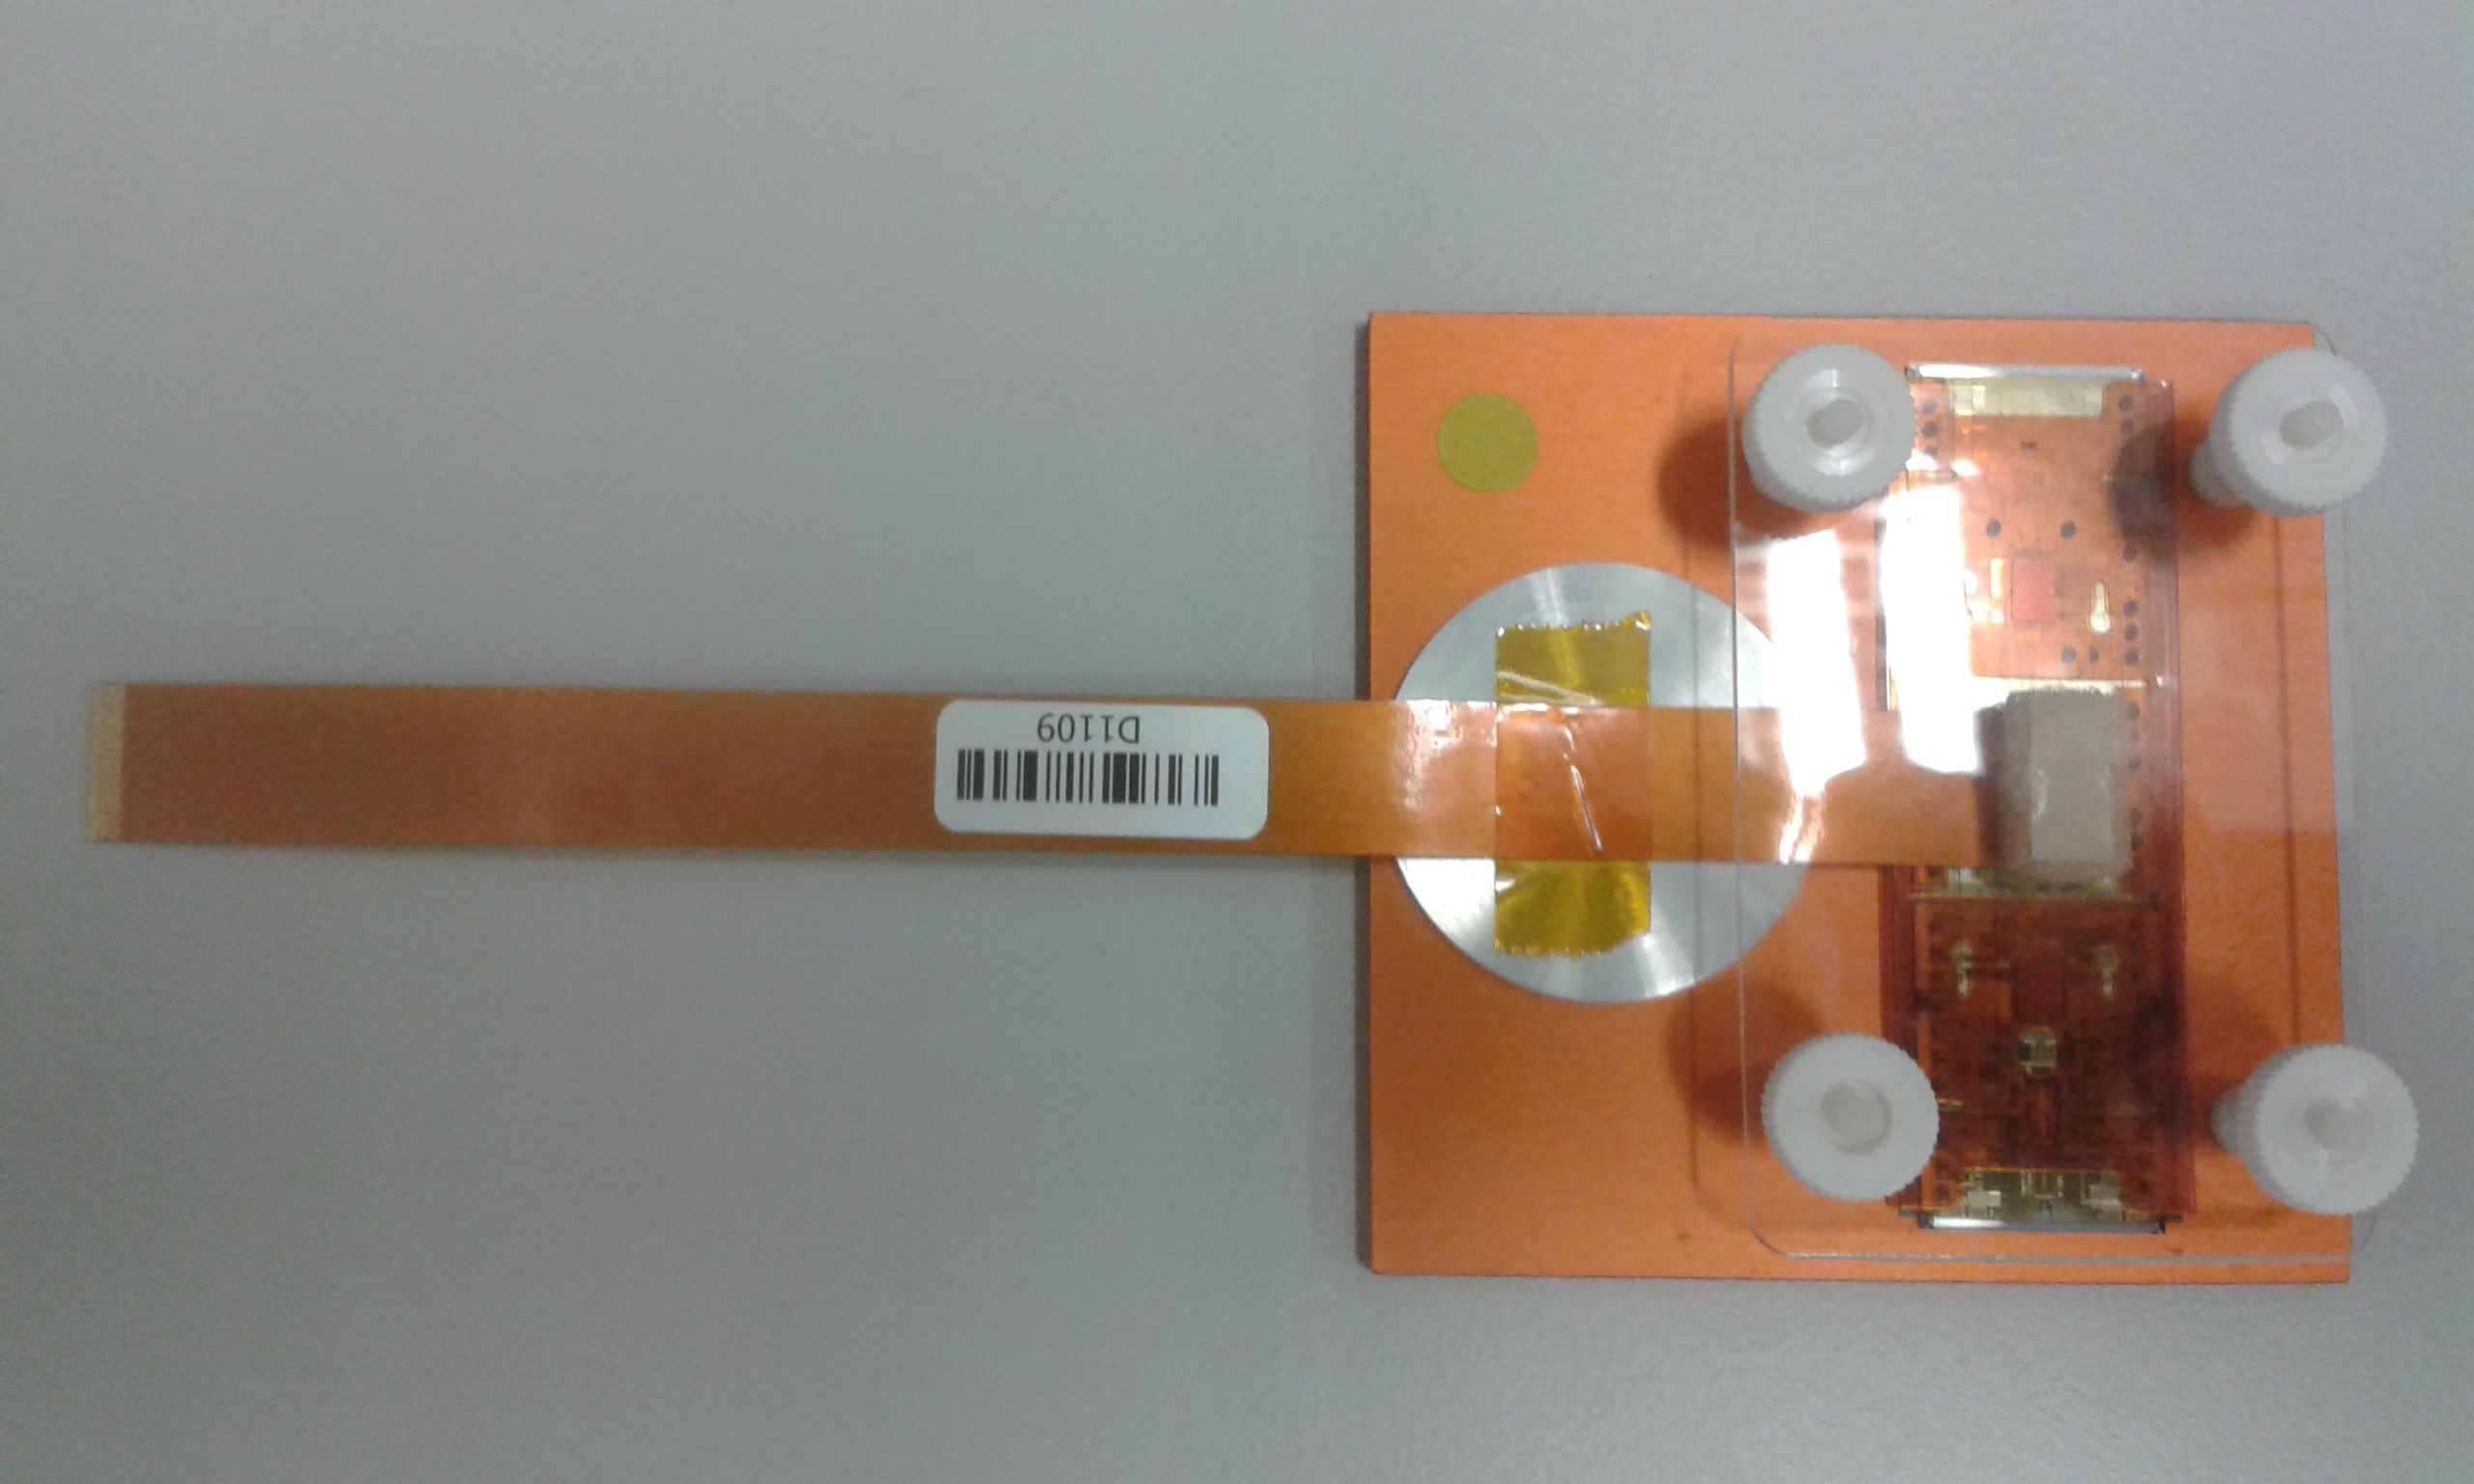
\includegraphics[width=\textwidth]{./L1.jpg}
  \caption{\em Picture of a L1 module}
  \label{L1}
\end{minipage}%
\hspace{1mm}
\begin{minipage}{.49\textwidth}
  \centering
  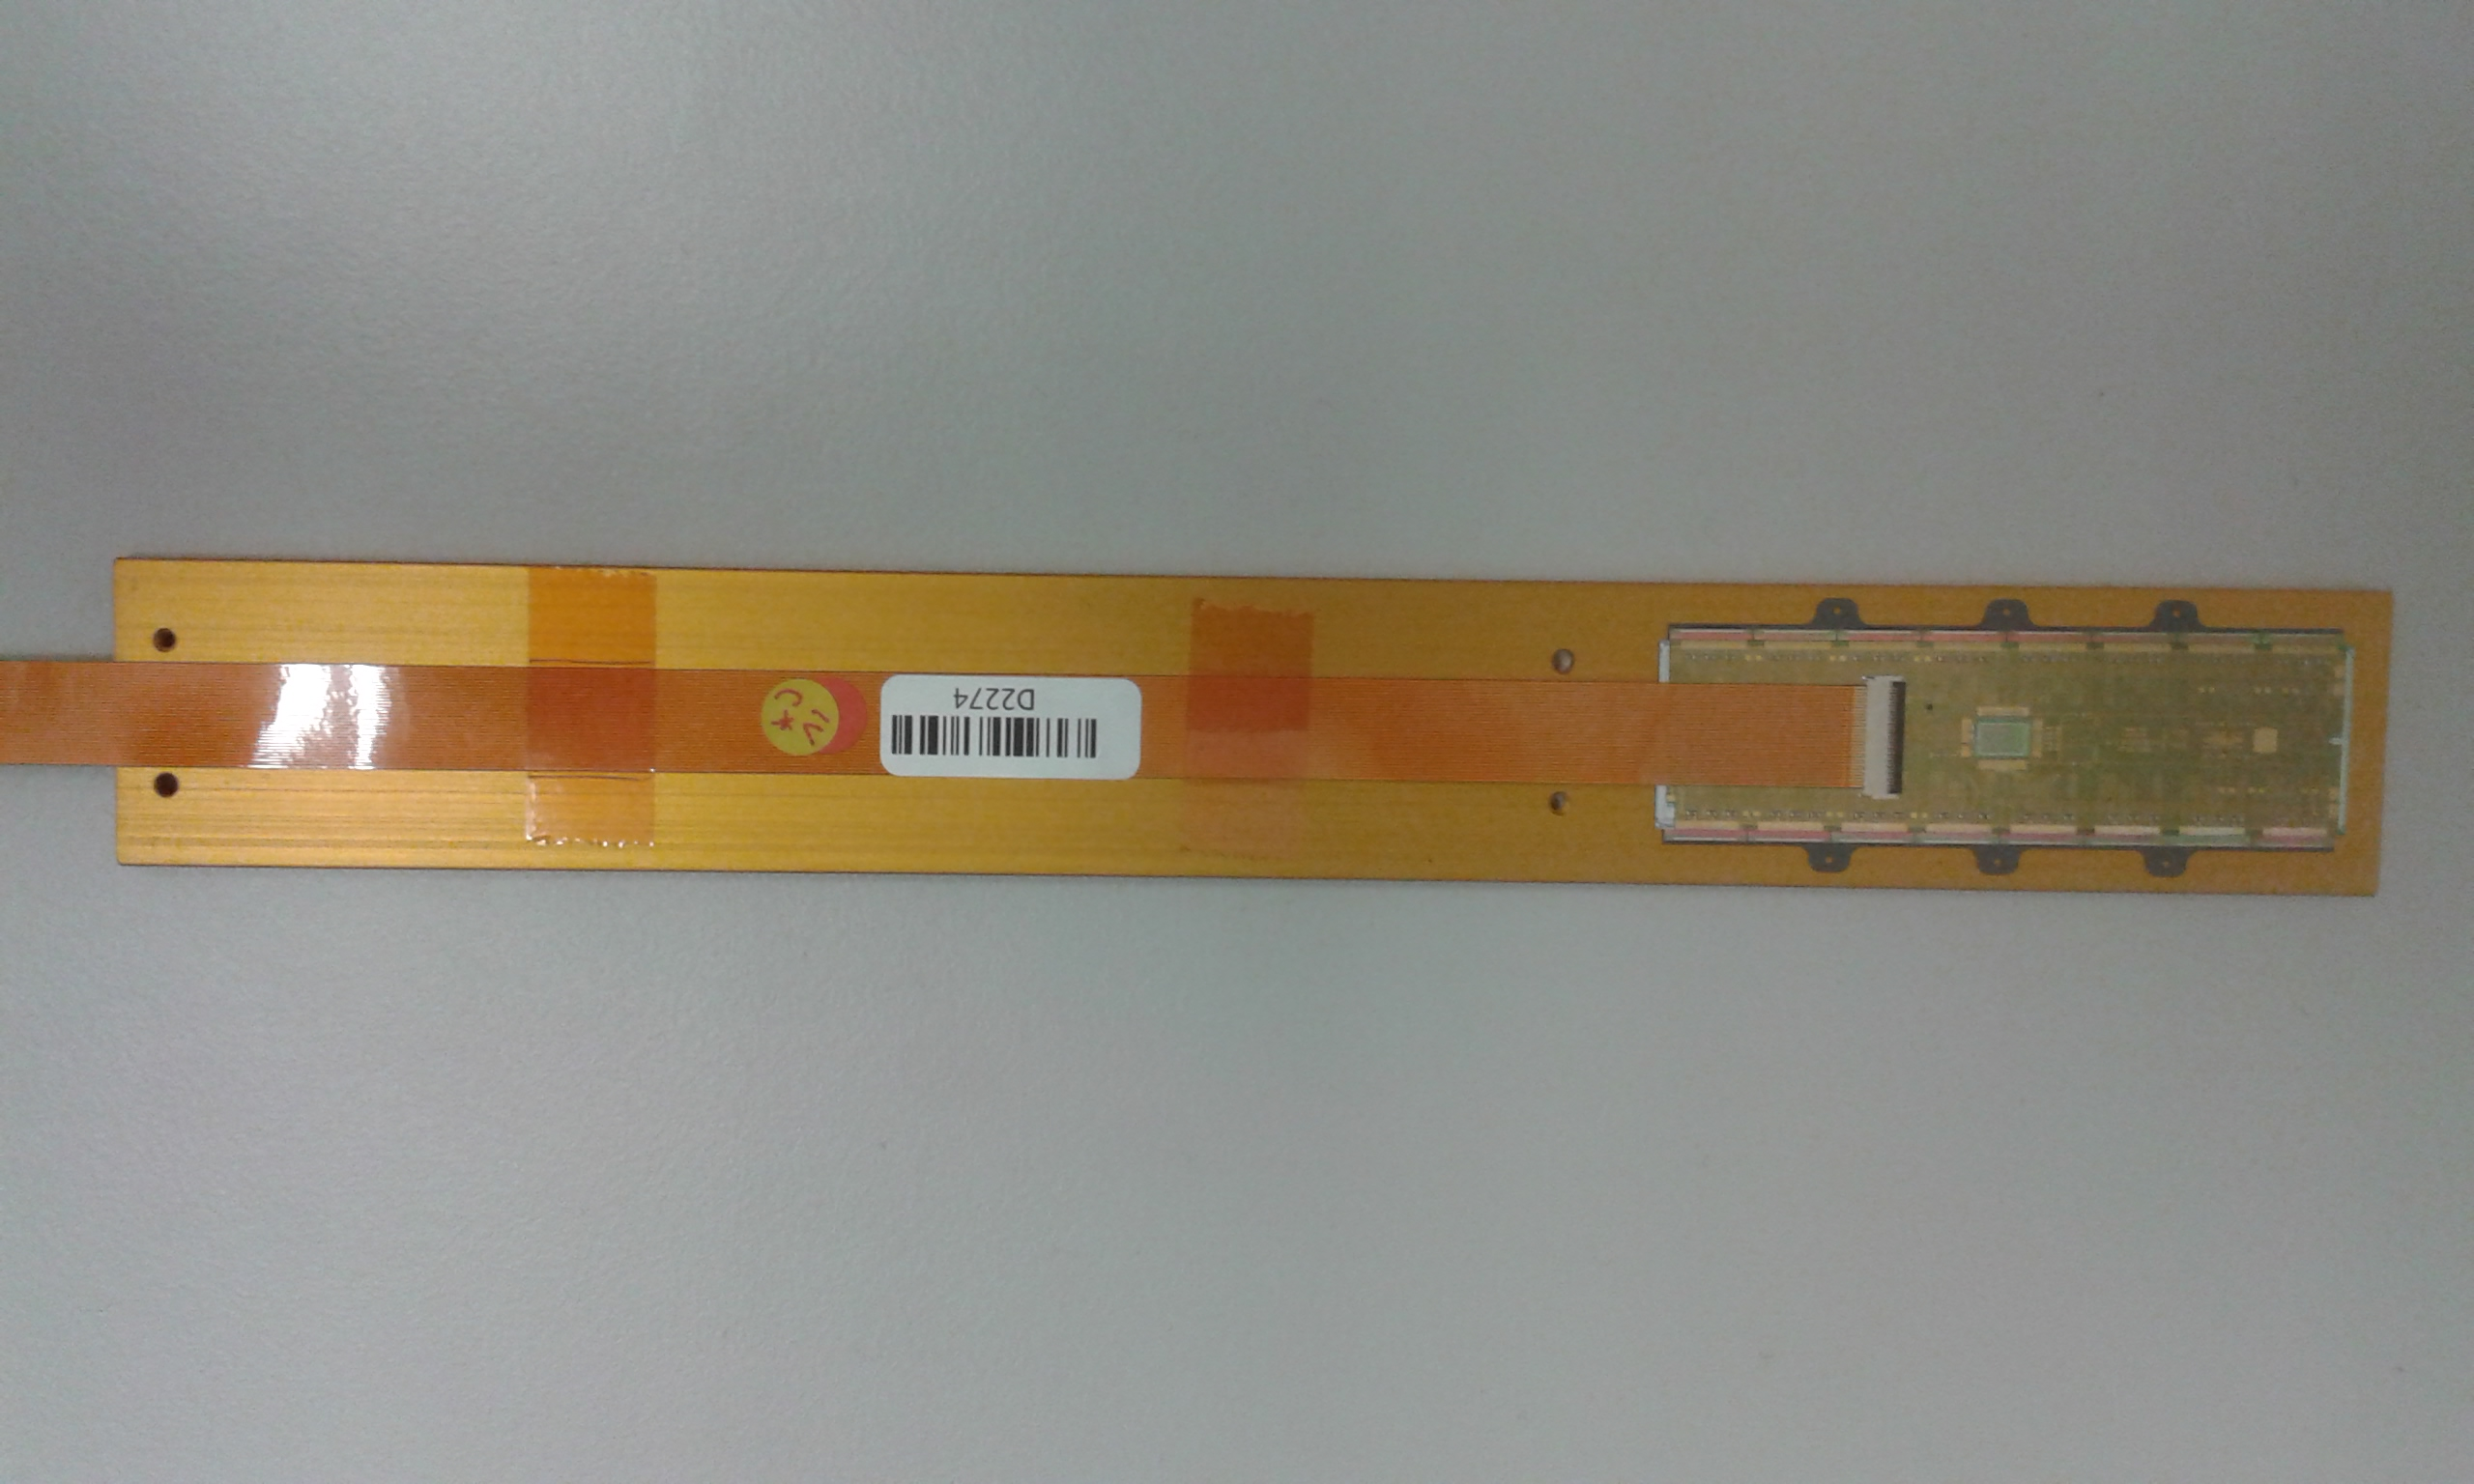
\includegraphics[width=\textwidth]{./L2.jpg}
  \caption{\em Picture of a L2 module}
  \label{L2}
\end{minipage}
\end{figure}

\section{Operation of the X-ray setup}  \label{Xraysetup}
The test setup (see Figure \ref{Setup}) is centred around an X-ray tube that has a chromium (Cr) anode. The radiation produced by the tube can either be used directly to obtain high particle rates or directed towards one of five metallic targets that produce a monochromatic but less energetic beam. The available targets are Iron (Fe), Copper (Cu), Molybdenum (Mo), Silver (Ag) and Tin (Sn). \\
Samples can be tested in a climatic chamber where air humidity is kept low and which can be cooled down to a desired temperature (up to -15$^\circ$C to -20$^\circ$C depending on the state of the Peltier elements and the water flux used for cooling). \\
A Keithley power supply is allocated to the setup which is used to provide a depletion voltage to the modules. \\
A PC is available for the execution of tests.

\begin{figure} [h!] \centering
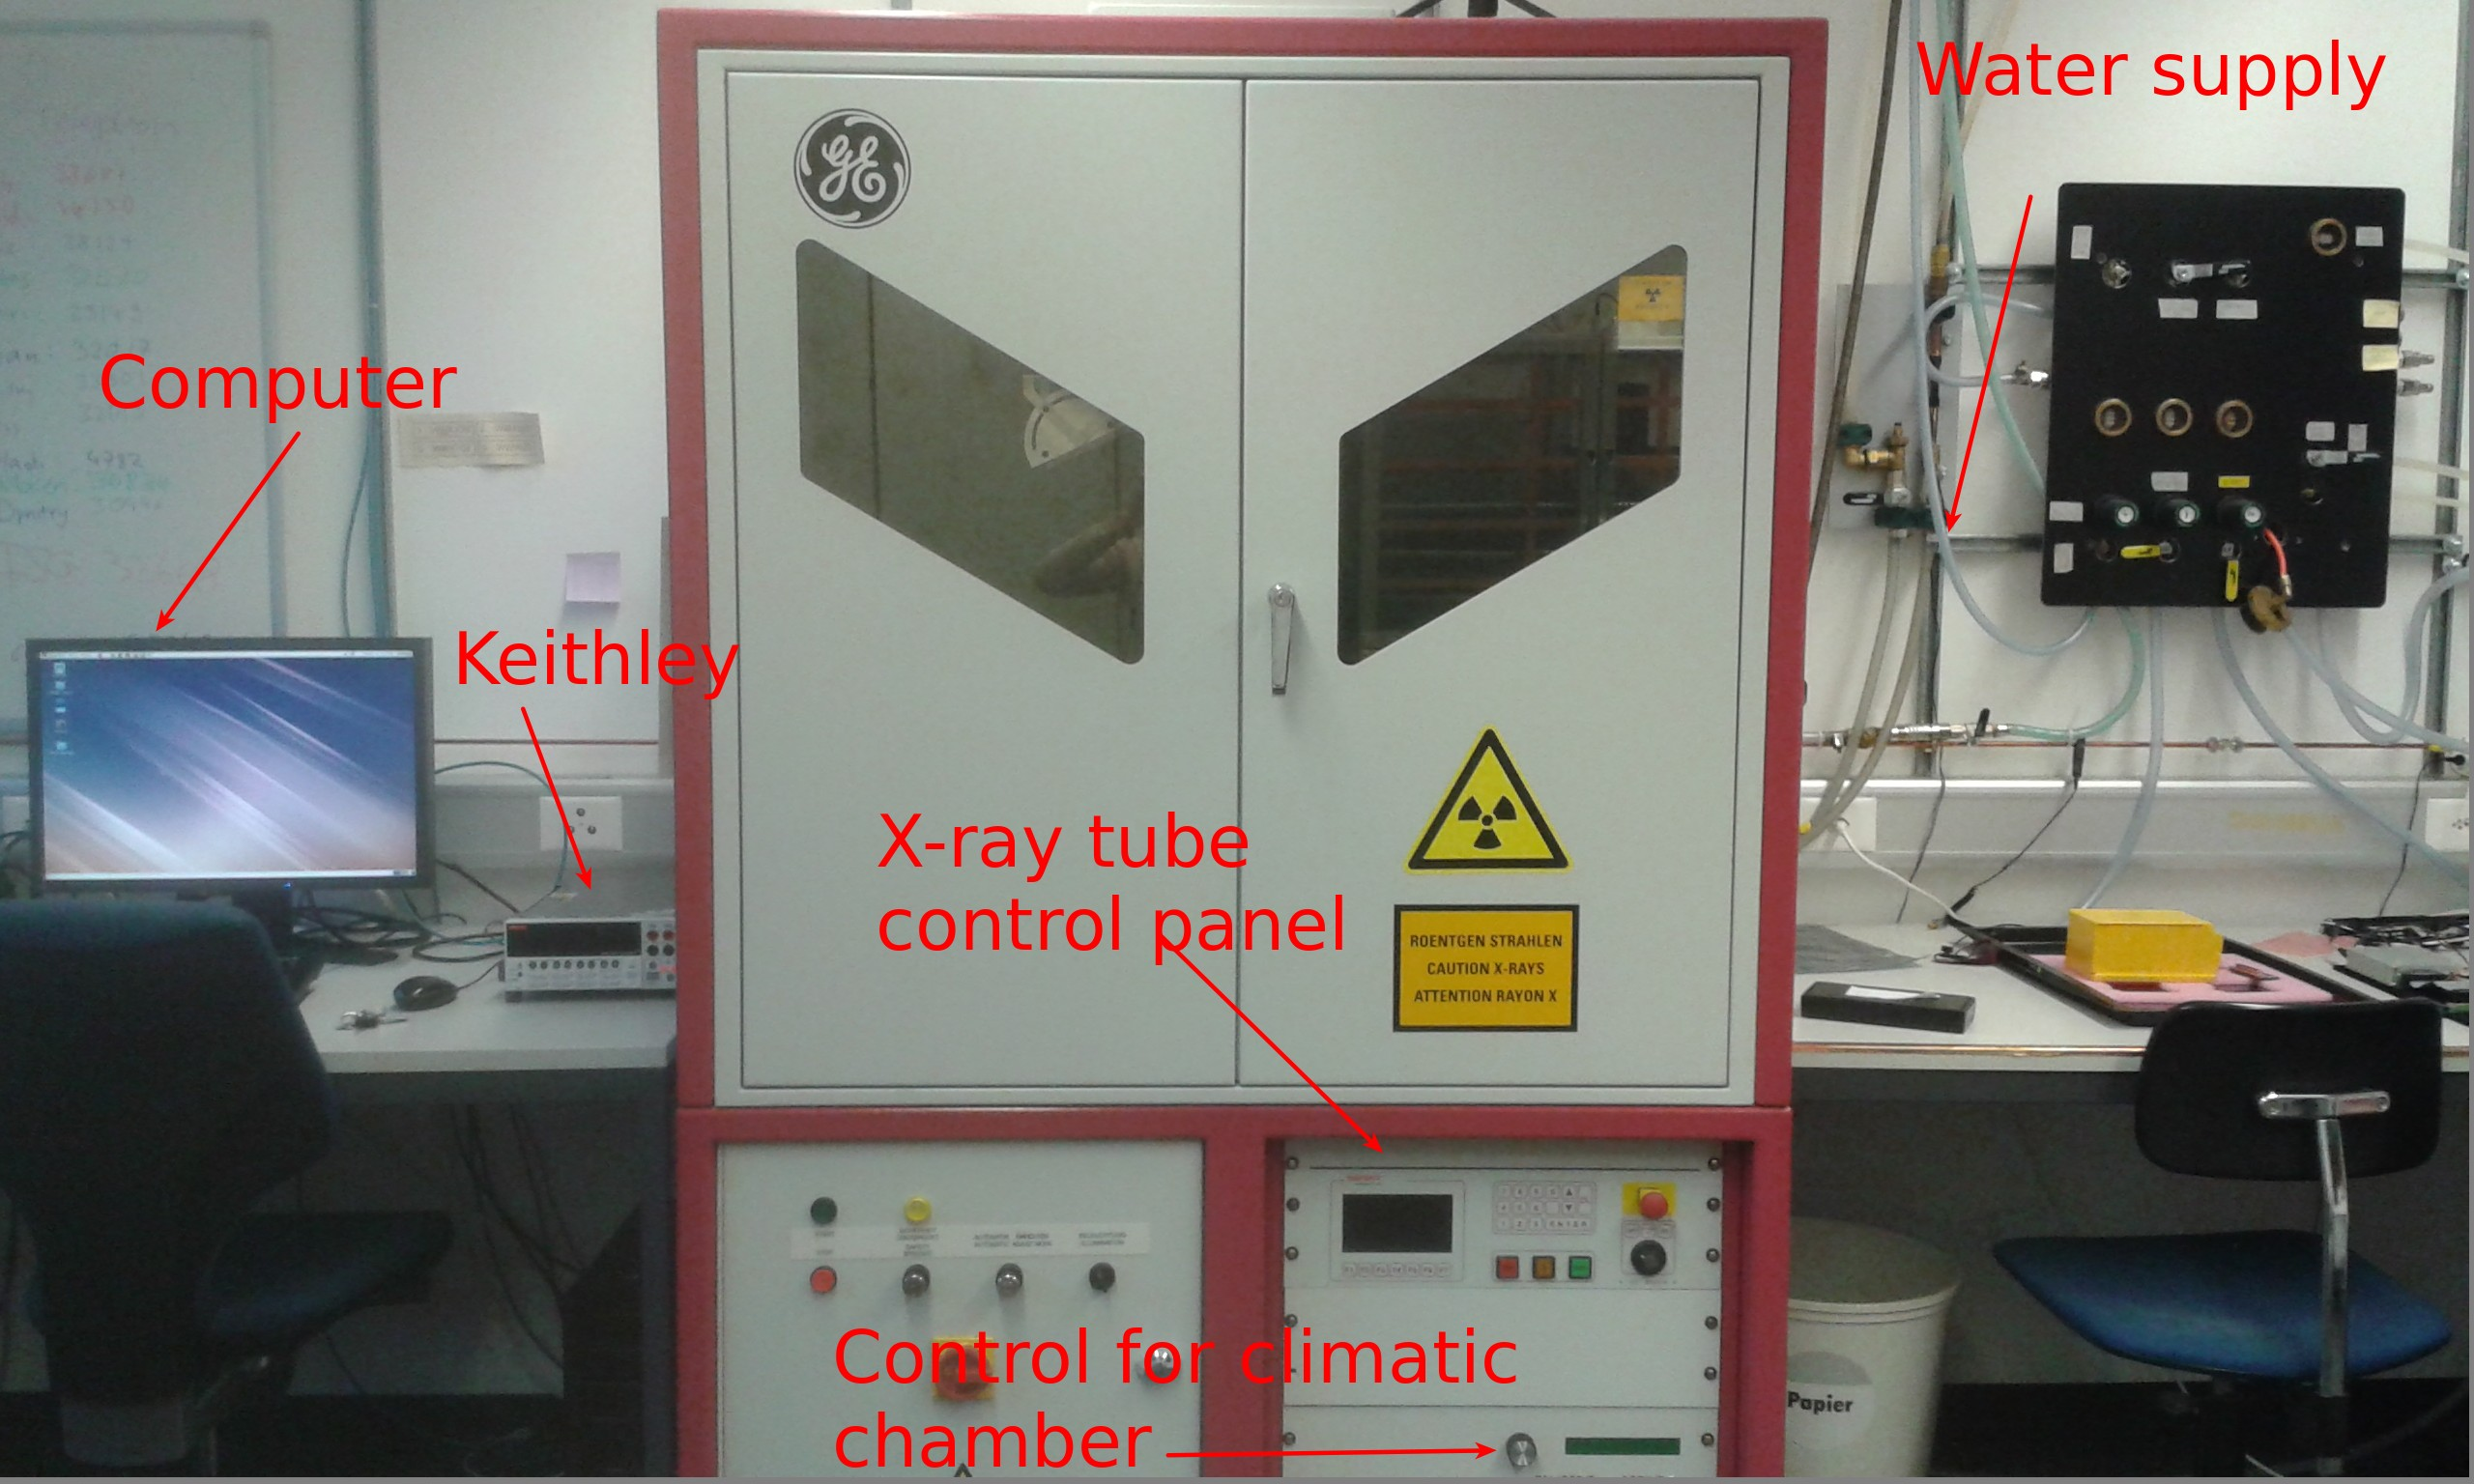
\includegraphics[width=\textwidth, angle=0] {./Setup.jpg}
\caption{\em  \label{Setup}
Picture of the X-ray testing setup including the X-ray tube, the control for the climatic chamber, the Keithley, the computer and the water supplies.}
\end{figure}


\subsection{Operation of the X-ray tube} \label{Operation}

One should be cautious when operating the X-ray tube since it produces highly energetic photons which can be harmful. 

\begin{itemize}
\item {Open valve entirely for X-ray cooling (3 on Figure \ref{Water}).
\begin{figure} [h!] \centering
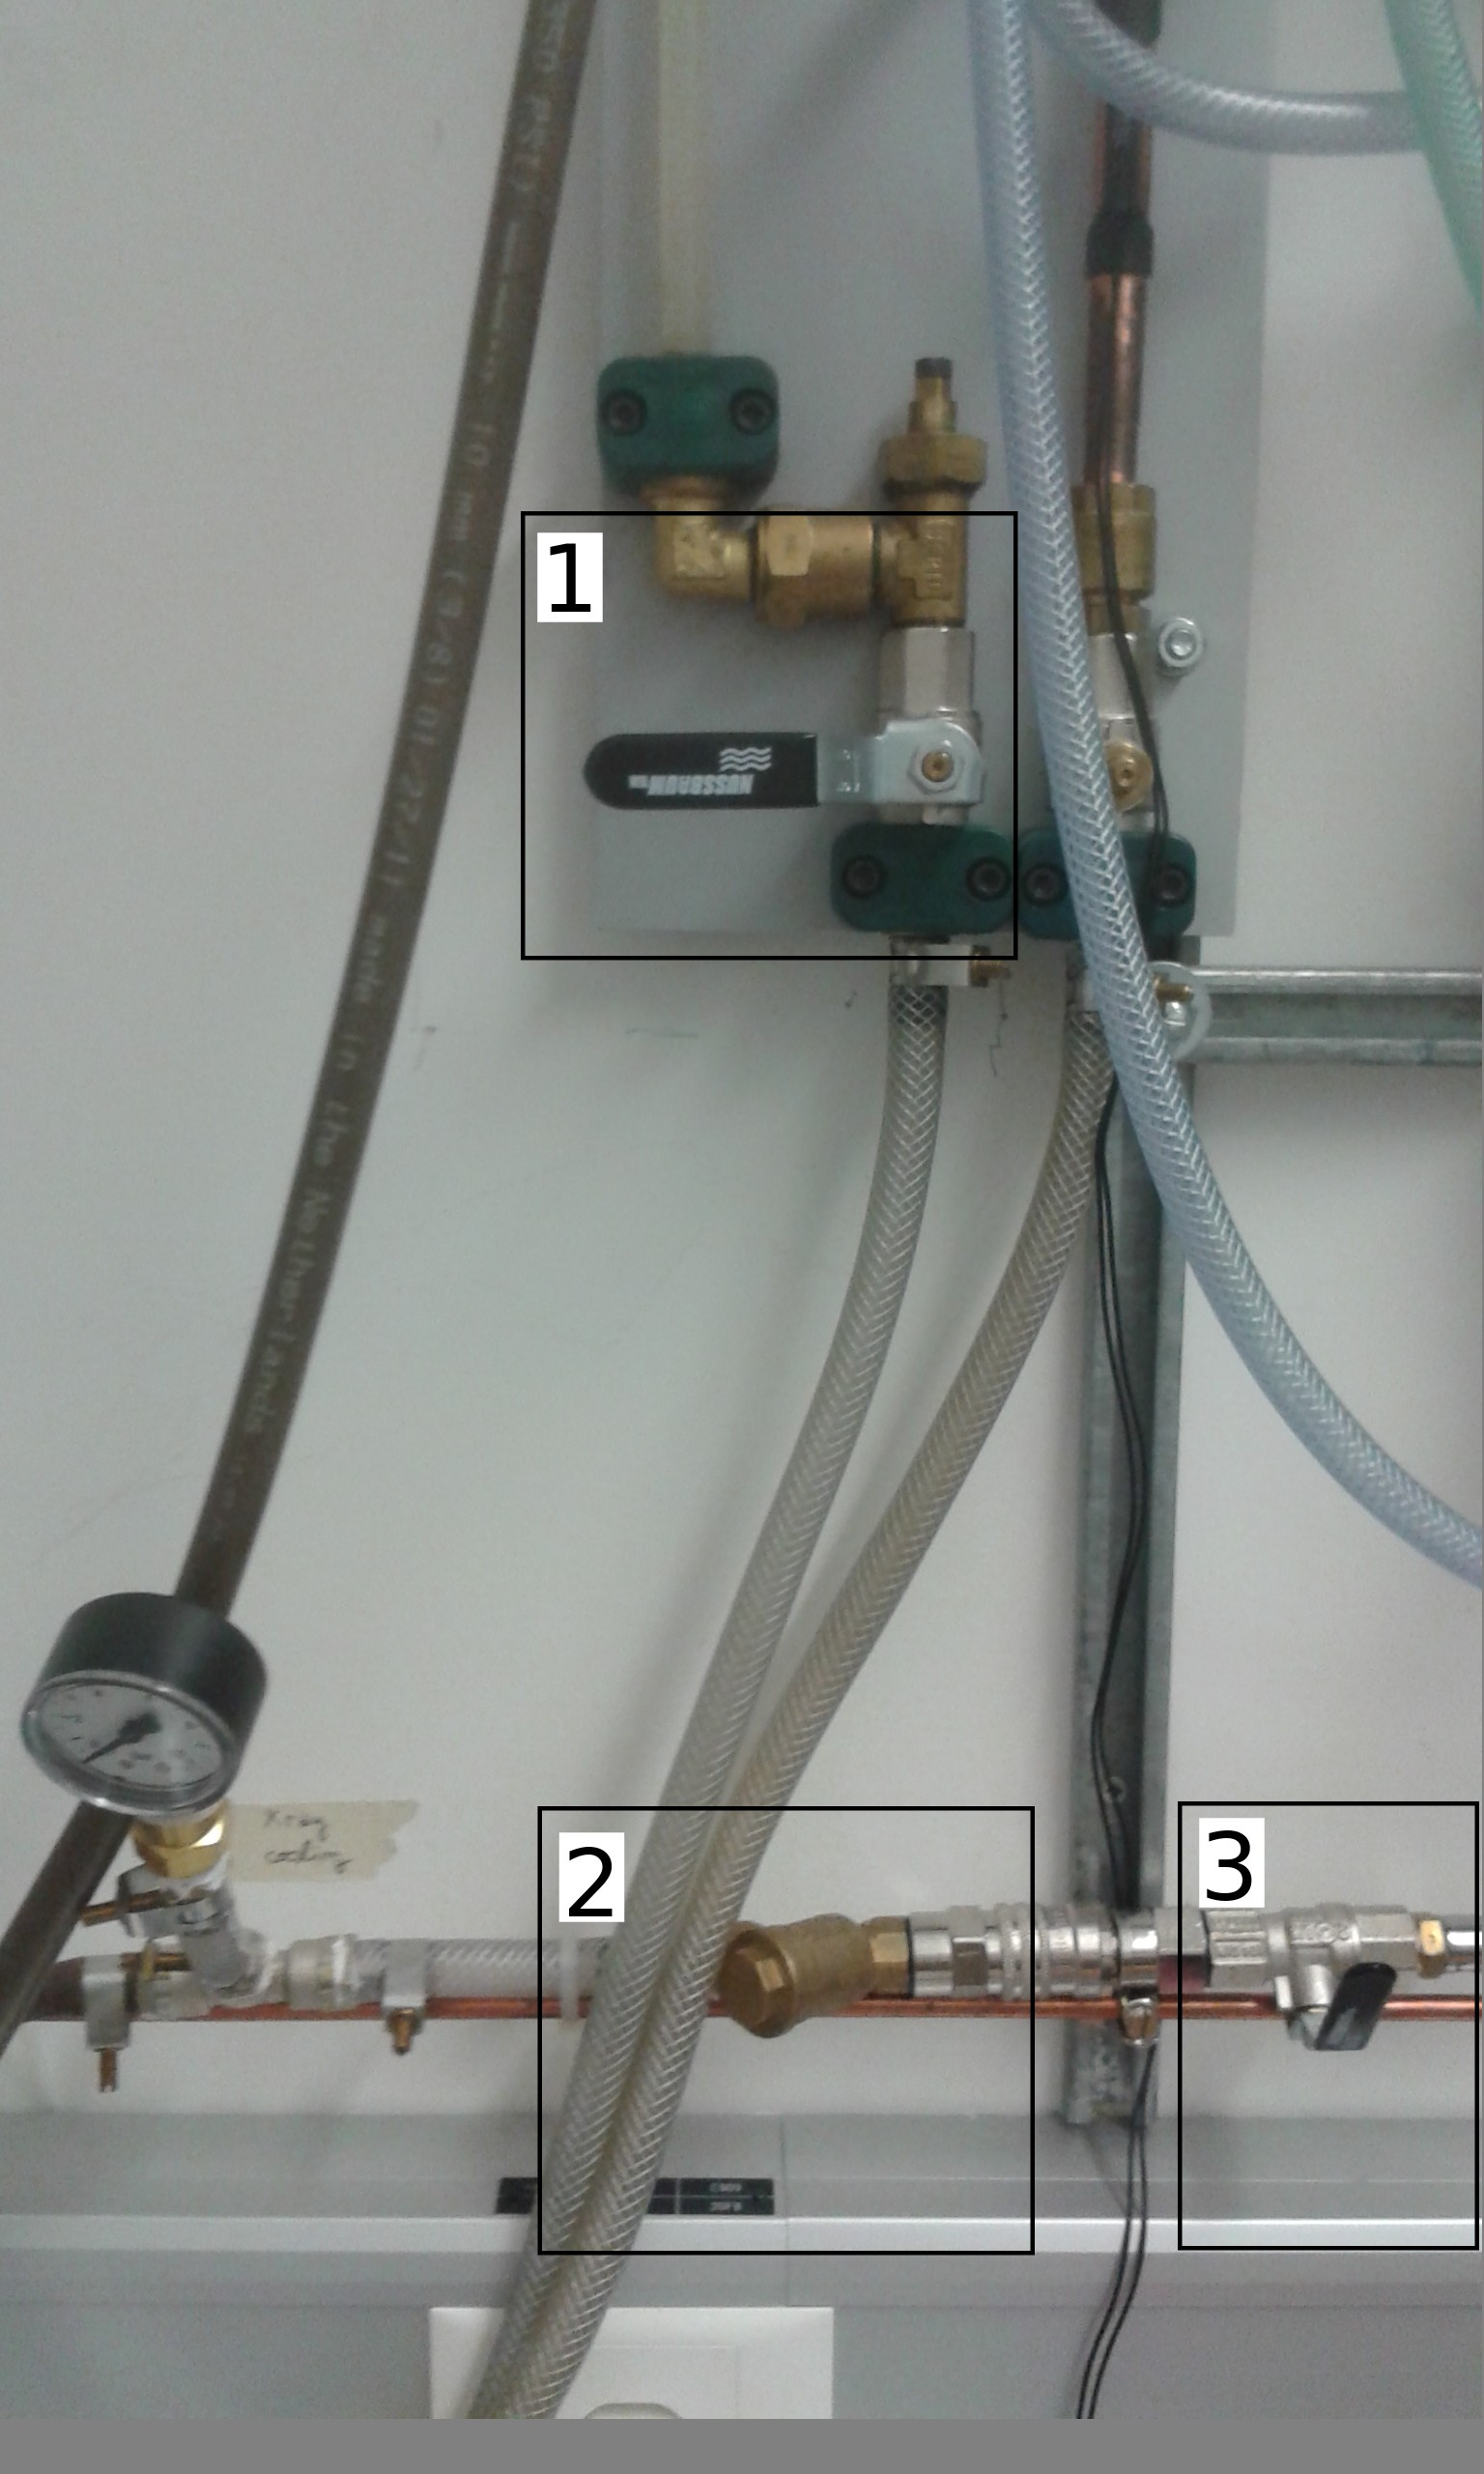
\includegraphics[width=0.5\textwidth, angle=0] {./Water2.jpg}
\caption{\em  \label{Water}
Picture of the water supply for the X-ray set up. Water supply 1 feeds the climatic chamber, supply 3 is used by the X-ray tube and filtered by 2.}
\end{figure}
}

\item {Switch on X-ray machine (3 on Figure \ref{Commandboard}).
\begin{figure} [h!] \centering 
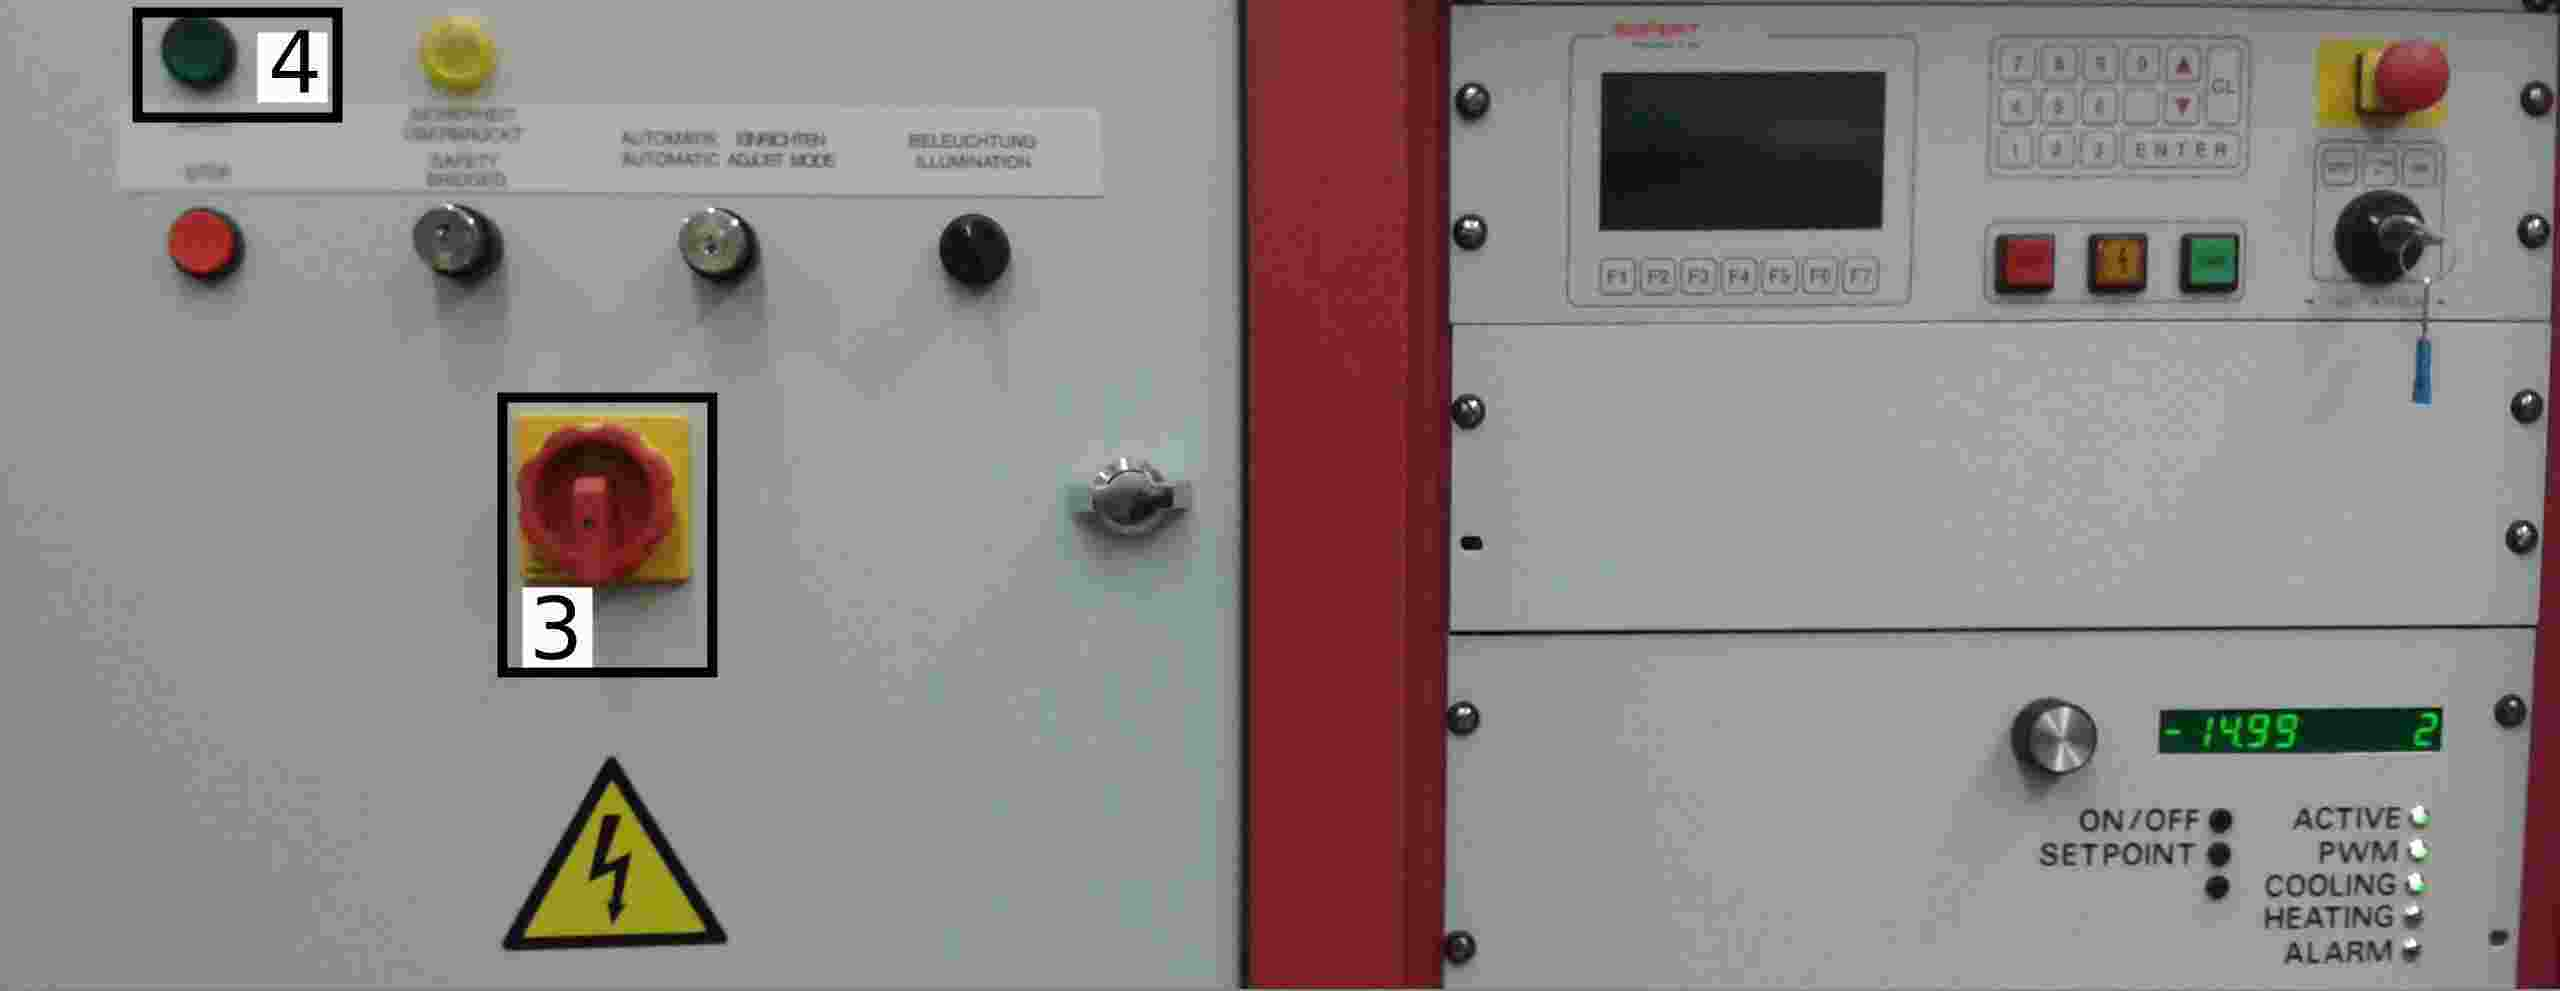
\includegraphics[width=0.9\textwidth, angle=0] {./Full2.jpg}
\caption{\em  \label{Commandboard}
Picture of the command board which enables to operate the X-ray tube and the climatic chamber.}
\end{figure}
}
\item {(Re)close the door of the X-ray setup housing, press round, green \textbf{START} button (4 on Figure \ref{Commandboard}).}
\item {Turn key to \textbf{ON}.
\begin{figure} [h!] \centering 
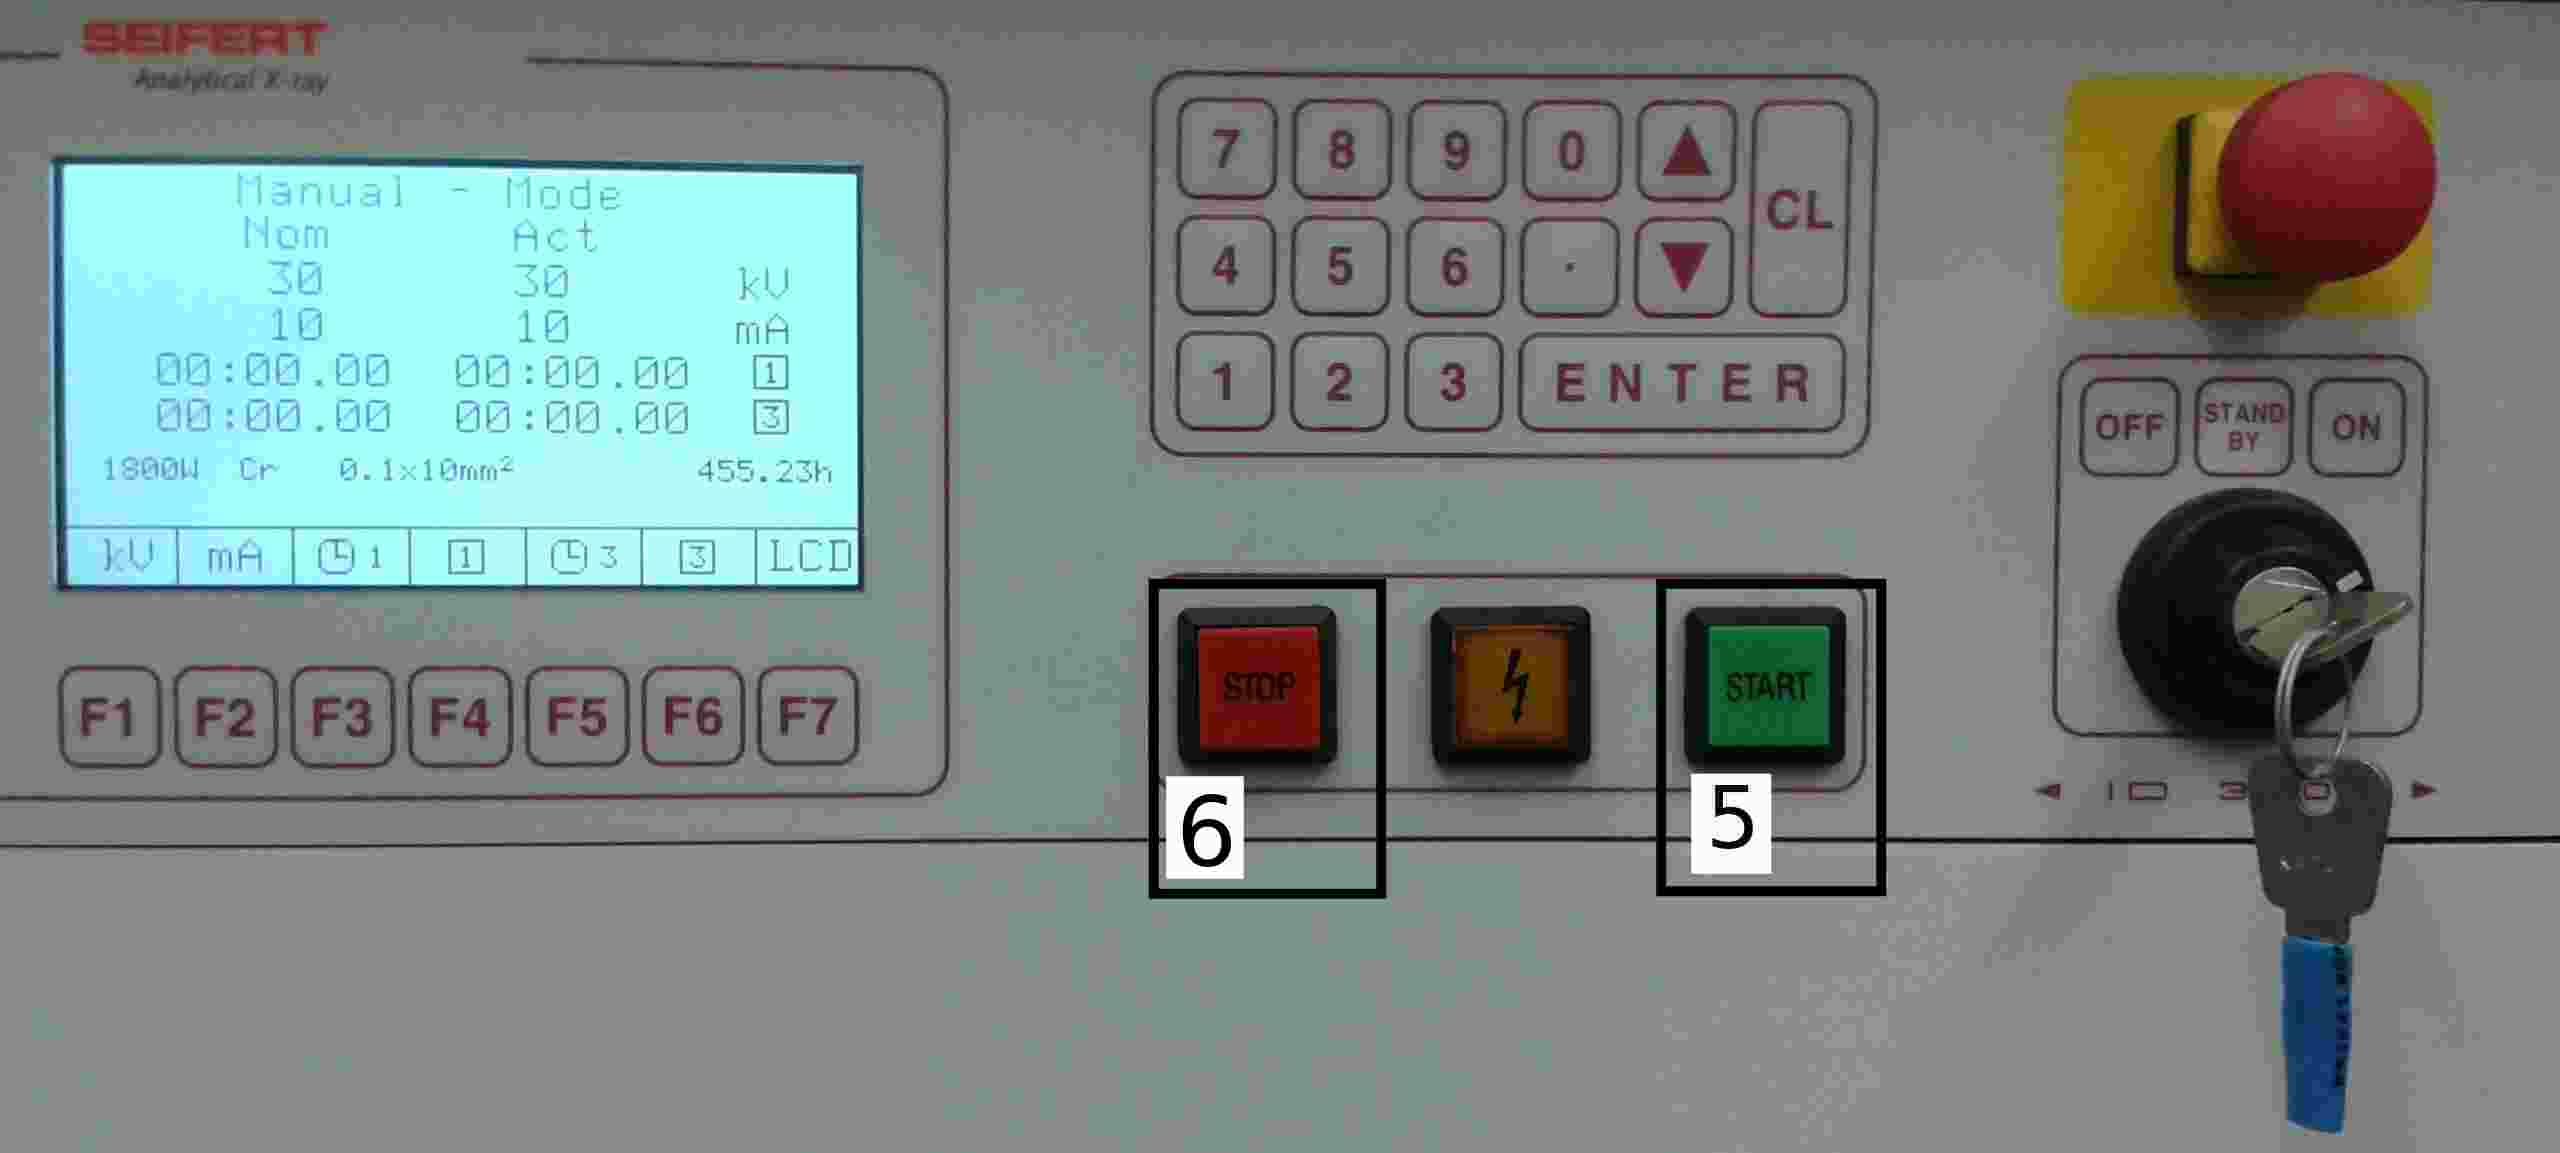
\includegraphics[width=0.9\textwidth, angle=0] {./CommandBoard2.jpg}
\caption{\em  \label{Xray}
Detailed picture of the control panel of the X-ray tube generator.}
\end{figure}
}
\item{Warm up X-ray tube by selecting \textbf{F7}. Enter the required current and voltage settings by selecting \textbf{F2, F4 or F6}. One shouldn't have very small values for currents with large voltages as well as the other way around. Suggested values are \SI{60}{\kV} and \SI{30}{\mA} for warming up the tube. Press \textbf{Enter} when finished, then \textbf{START} (square green one, 5 on Figure~\ref{Xray}). This will take up to 30 minutes depending on when the tube was operated the last time at this or a higher voltage. If the voltage is not set, check green interlock button (4) and the door, press \textbf{CL} to delete the error message.}
\item {To control X-ray tube settings during operation, use the \textbf{id3003} which is installed on the computer. With this, the X-ray generator can be shut on and off, the voltage and current settings can be adjusted, and the shutter opened and closed. Shutter 1 directs the beam to the targets, shutter 3 directs it directly to the modules. Some examples:
\\
\\
\begin{Verbatim}[frame=single]
id3003.py open shutter 1
id3003.py close shutter 1
id3003.py set hv on
id3003.py set hv off
id3003.py set voltage 30
id3003.py set current 10
id3003.py get voltage
id3003.py get current
\end{Verbatim}
}
\item{When taking a break, turn off high voltage and close the shutter. Turn key to \textbf{STAND BY}.}
\end{itemize}
After use, turn off the set up as follows:
\begin{itemize}
\item {Close the shutter, turn off high voltage.}
\item {Press \textbf{STOP} (6 on Figure~\ref{Xray}).}
\item {Turn key to \textbf{OFF}.}
\item {Turn off X-ray machine.}
\item {Close water valve.}
\end{itemize}
\subsection{Targets for monochromatic X-ray beam}

The set-up is equipped with a movable holder that holds five metallic plates used to create a monochromatic beam. 

\begin{figure} [h!] \centering 
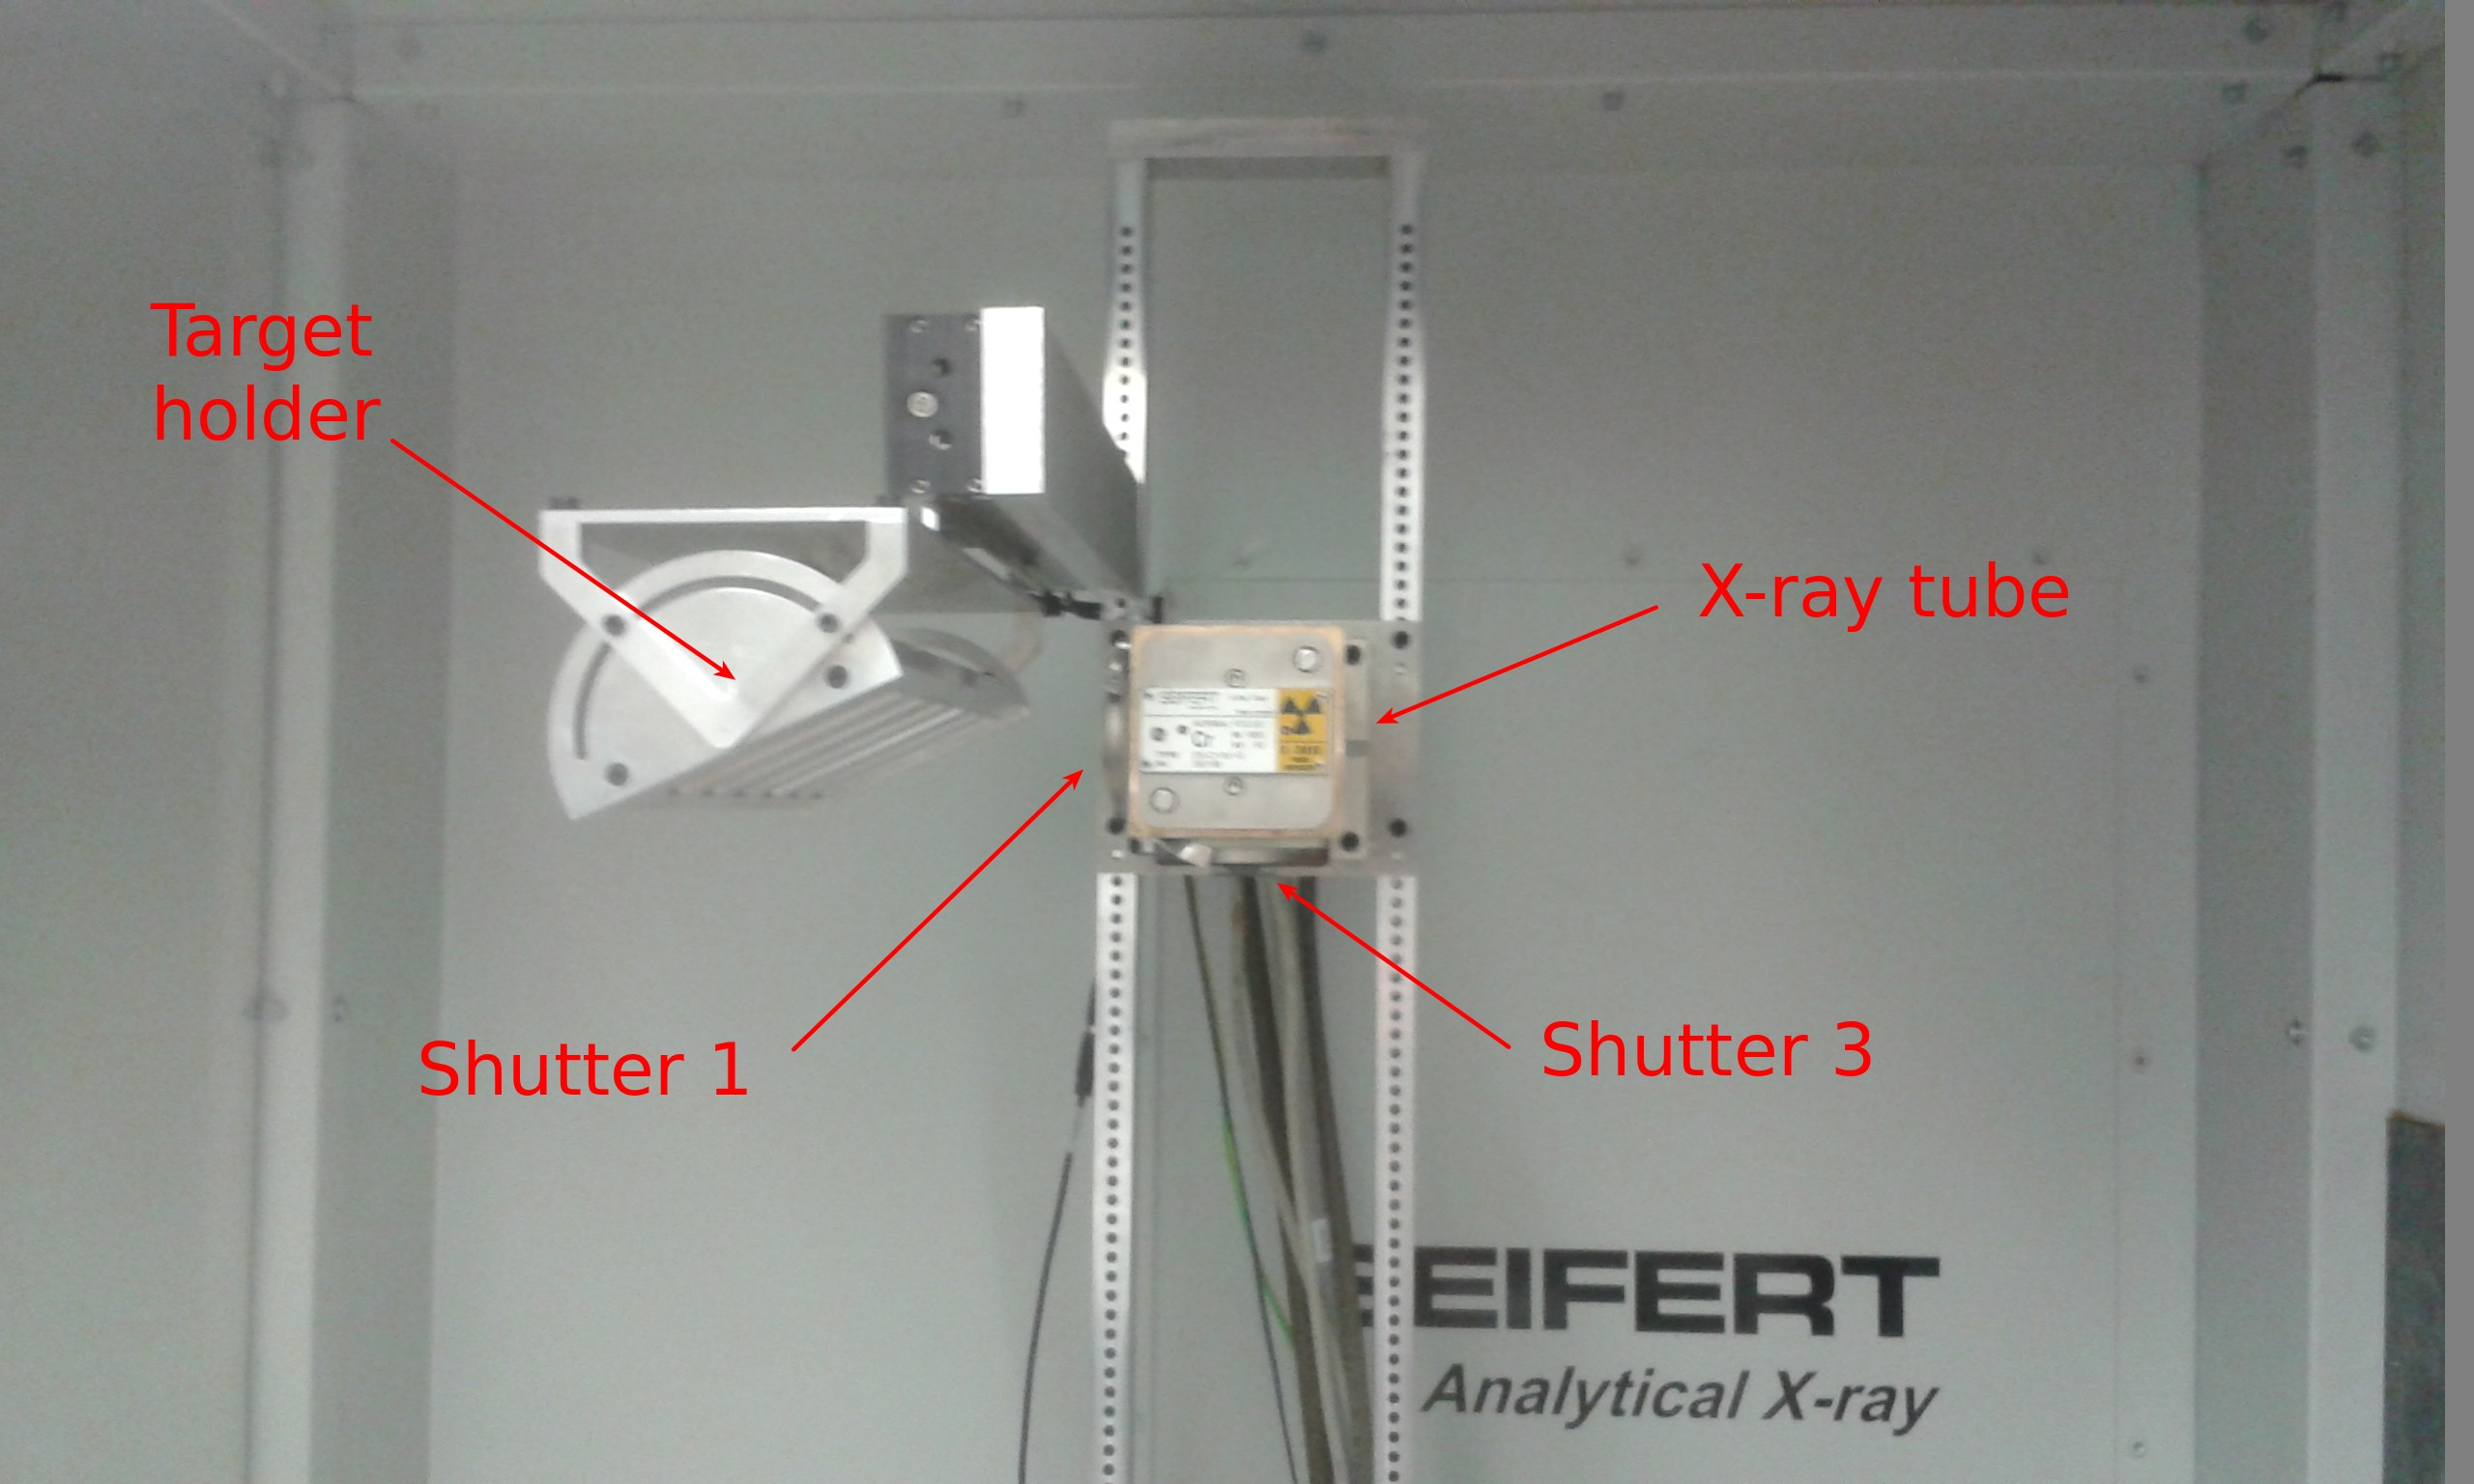
\includegraphics[width=0.9\textwidth, angle=0] {./Targets.jpg}
\caption{\em  \label{Targets}
Picture of the target holder and the two shutters of the X-ray beam.}
\end{figure}

\begin{itemize}
\item {To change the target during operation, the \textbf{xrf} program is needed.  Available targets are Zn, Cu, Mo, Ag, Sn. Some examples:
\begin{Verbatim}[frame=single]
xrf Ag
xrf Mo
xrf Screen
\end{Verbatim}
}
\end{itemize}

\subsection{Climatic chamber}

The climatic chamber creates an temperature and humidity controlled environment to test modules. The chamber is continuously flushed with dry nitrogen to keep the humidity low. Six Peltier elements \footnote{Type C2-50-1514 from \url{www.tellurex.com}} are used to cool down the chamber to up to -20$^\circ$C.

\begin{itemize}
\item Open valve for module cooling (2 on Figure~\ref{Water}) until the pressure is about \SI{2}{\bar} (check with left barometer in the X-ray setup). The water pressure is relevant as the minimum temperature to which the box can be cooled down to depends on it. 
\item Switch on cooling with the \textbf{ON/OFF} button
\item Choose setpoint by pressing button \textbf{SETPOINT} while turning the knob at the same time.
\item After use turn the cooling off by pressing the \textbf{ON/OFF} button and closing the water valve.
\end{itemize}

\subsection{Keithley}
The Keithley power supply is used to provide a depletion voltage to the sensors of the modules. 

\begin{figure} [h!] \centering 
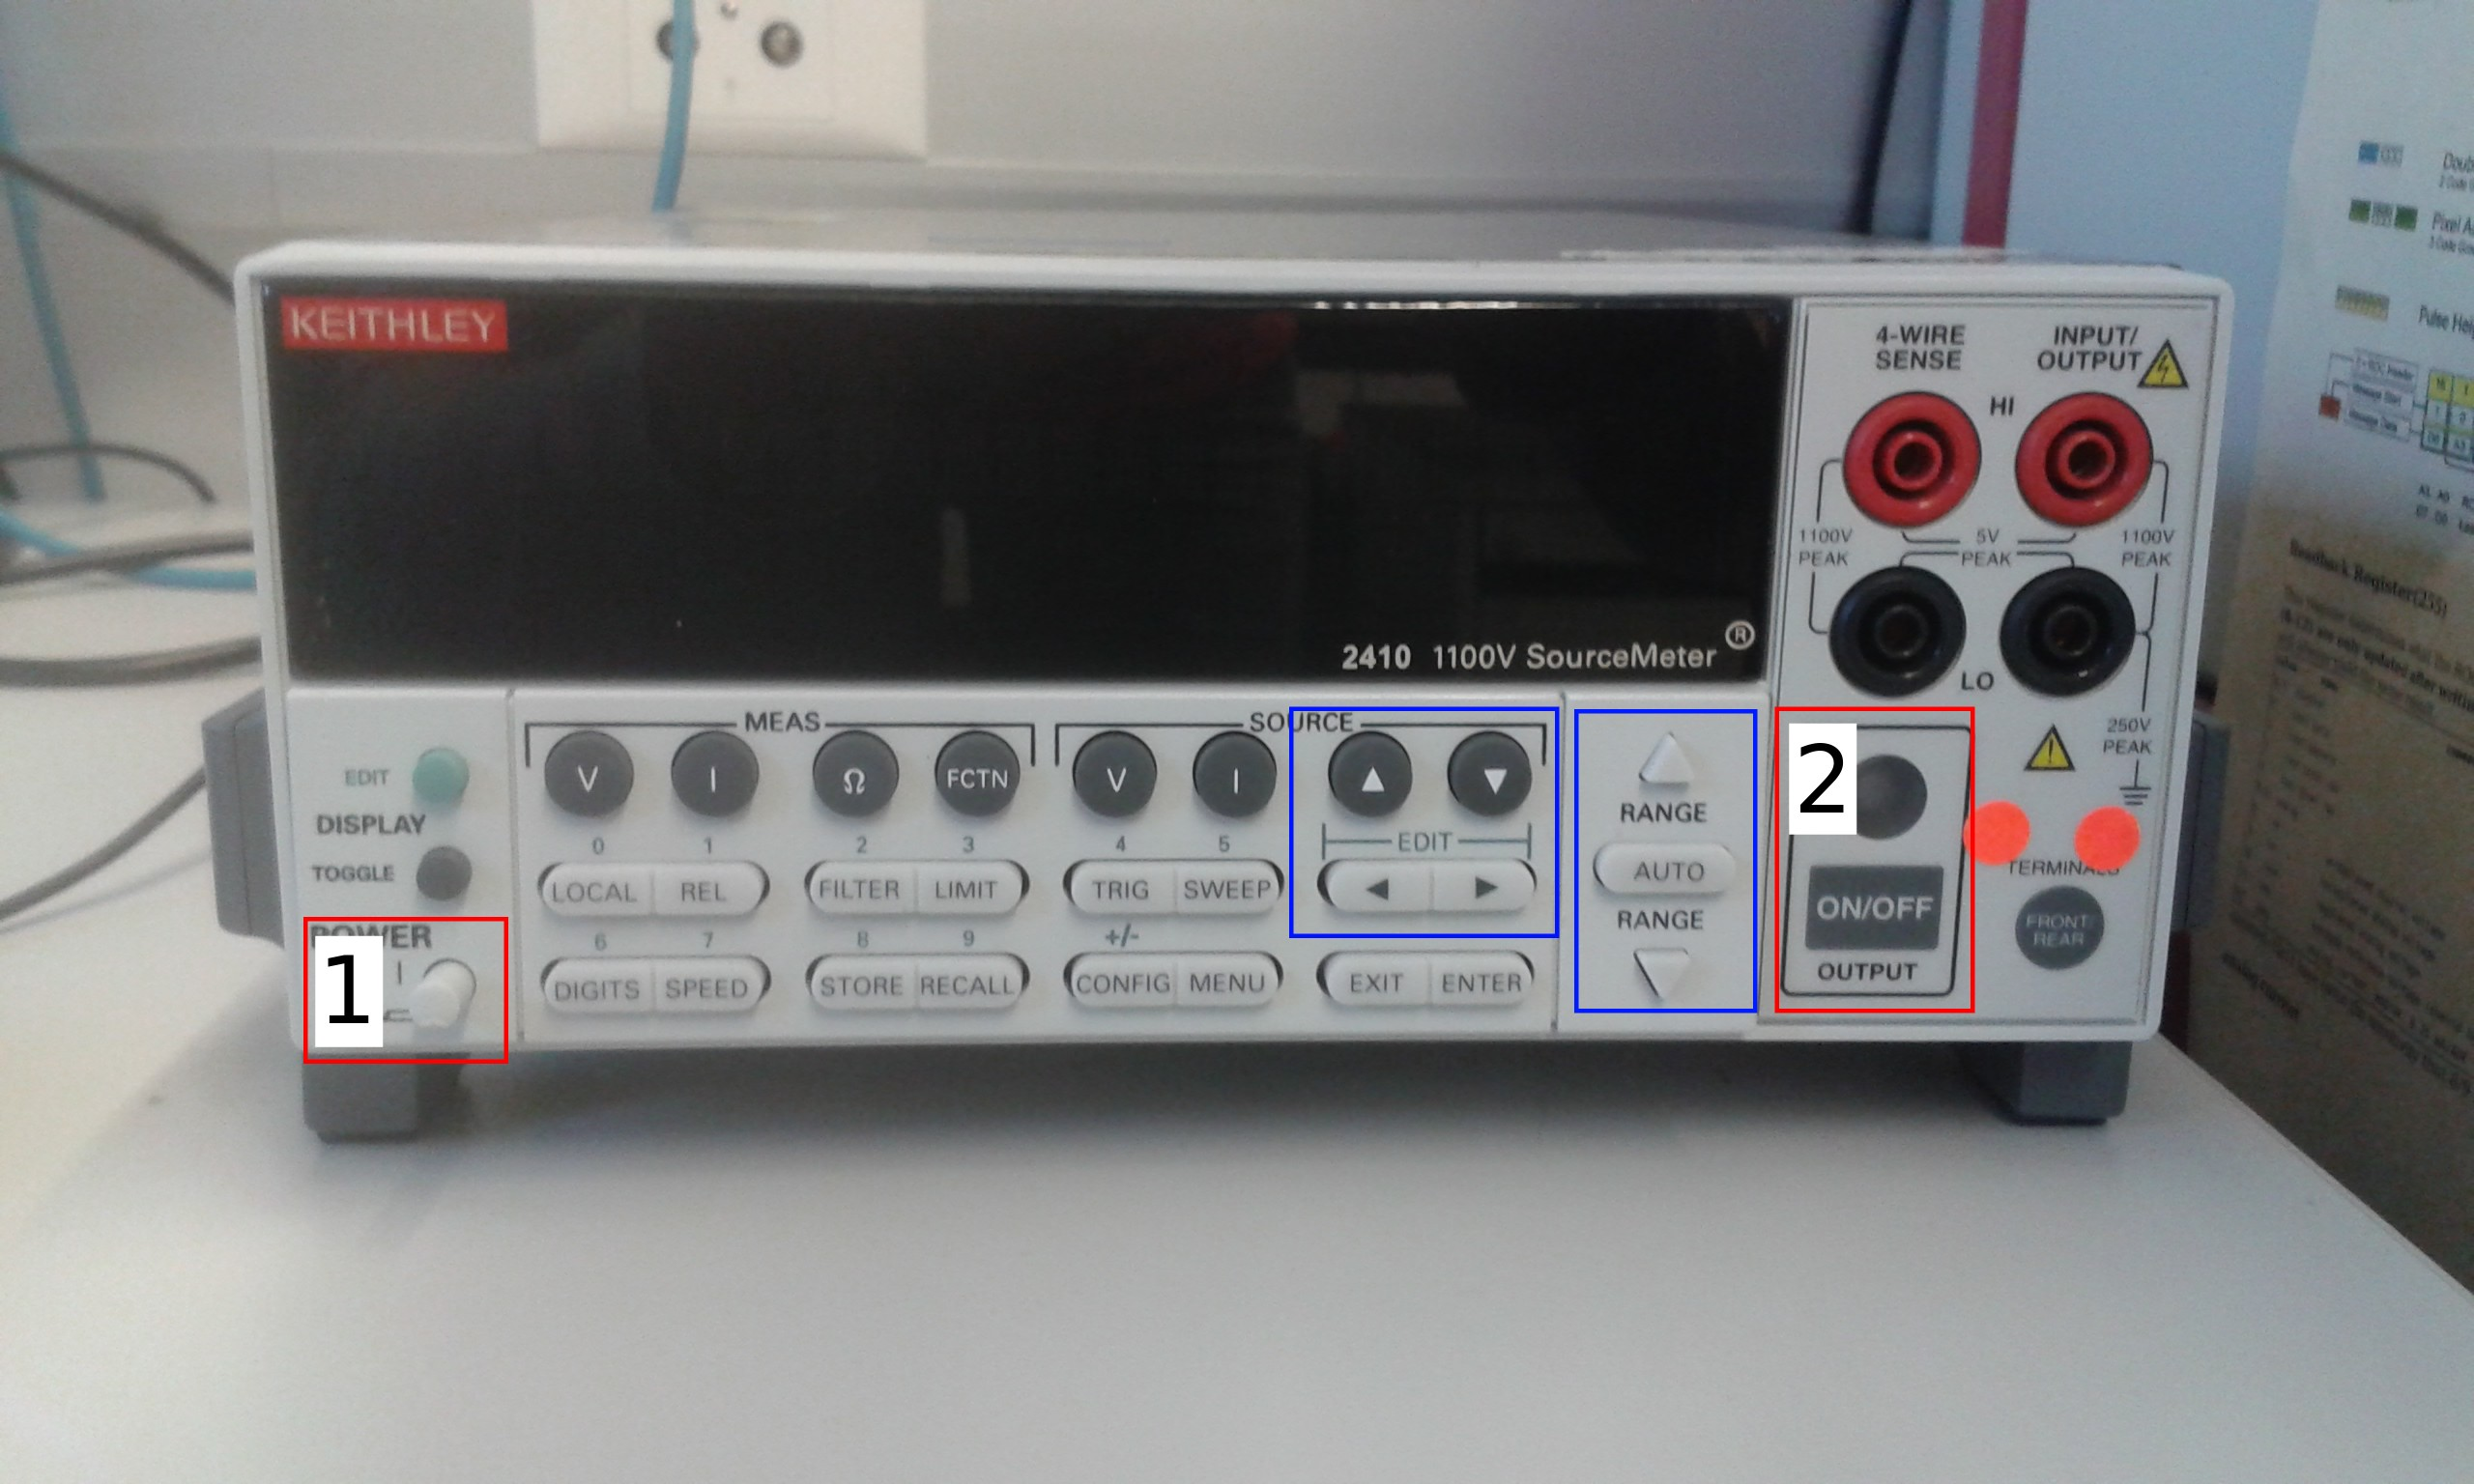
\includegraphics[width=0.9\textwidth, angle=0] {./Keithley.jpg}
\caption{\em  \label{Keithley}
Picture of the Keithley power supply.}
\end{figure}
\begin{itemize}
\item Turn on Keithley by pressing 1 on Figure~\ref{Keithley}.
\item Choose desired bias voltage with the buttons marked in blue on Figure~\ref{Keithley}.
\item Apply bias voltage to module by pressing button 2 on Figure~\ref{Keithley}.
\end{itemize}

\subsection{Troubleshooting}
Here are some issues that can occur during the use of the X-ray set up and a solution:
\begin{itemize}
\item Door of the X-ray setup is not closed properly: "Emergency stop" appears on the display when one tries to start the tube. Make sure to properly close the door and to press green \textbf{START} button (4) before retrying.
\item Climatic chamber is not reaching low temperatures. Try adjusting the water flow. If this does not help, one or several Peltier elements might be faulty. Replace them using the description in Appendix~\ref{Peltier}.
\item Error message saying that the water flow is too low. If it was forgotten to open the water valve, do this and start over. Otherwise, the flow is too low due to dirty filters. Check external filter on the wall (2 on Figure~\ref{Water}) first which is easier to clean. Unscrew and clean the filter with water and dry air. If this does not solve the issue, one needs to clean the built-in filter in the X-ray tube casing. This is a very delicate operation due to the sensitive berillium windows in the tube. This should only be performed by someone who has done this before. Instructions for it can be found in Appendix~\ref{Filter}.
\item Targets do not move. Scroll the targets to the "back" position manually.
\item X-ray tube in December 2016 is at the end of its lifetime, so it will likely stop working in the near future. The ETH pixel group is in possession of a replacement tube. Appendix~\ref{Filter} explains how to access to the tube for it to be exchanged. 
\end{itemize}


\section{Module testing set-up}

The set-up for testing L1 and L2 modules differs slightly. It is possible to test up to two L1 or four L2 modules at the same time.

\begin{figure} [h!] \centering 
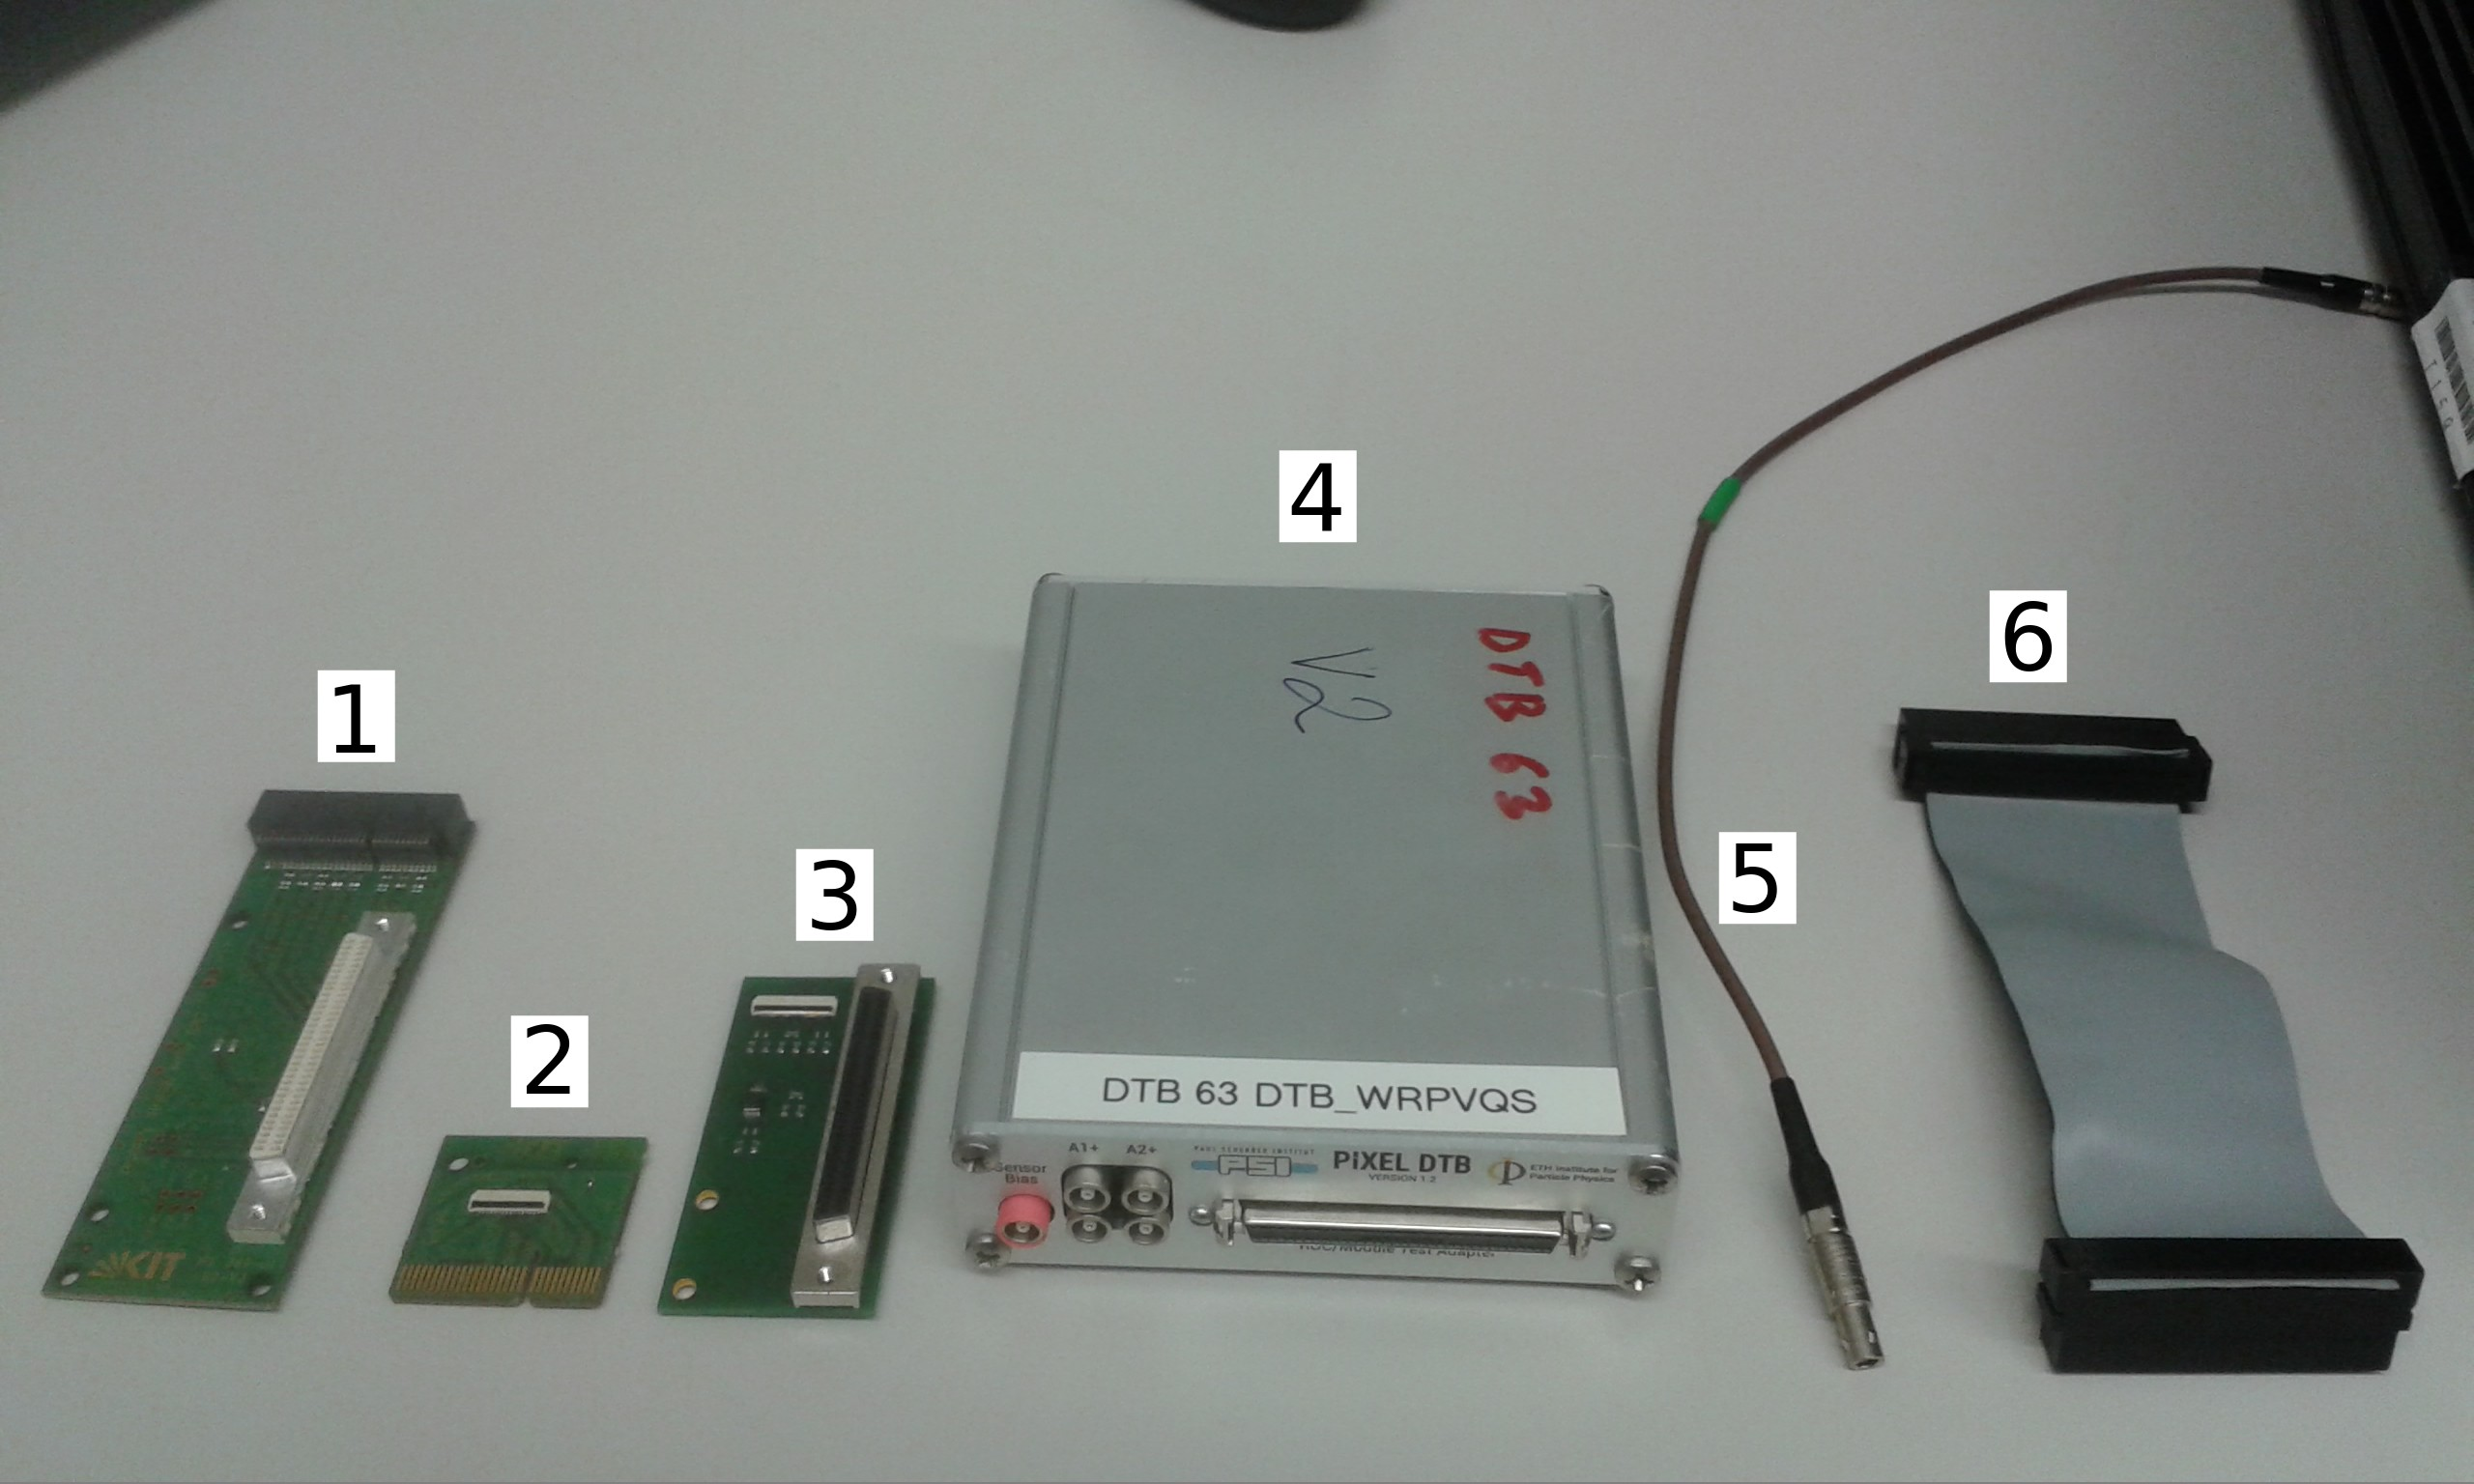
\includegraphics[width=0.9\textwidth, angle=0] {./Material.jpg}
\caption{\em  \label{Material}
Picture of the material needed for L1 and L2 modules. 1 is the module adapter for L2 modules, 2 the adapter card for L2 modules, 3 the module adapter for L1 modules, 4 the Digital TestBoard, 5 the LEMO cable, 6 the flatband cable.}
\end{figure}

In addition to the components of the set up listed above, the material needed for the qualification consists of:

\begin{itemize}
\item One Digital TestBoards (DTBs) including power and USB cable per module
\item One flatband cable and module connector (L1 or L2) per module
\item One insert card for each L2 module
\item 1 LEMO cable per module connecting the Keithley to the DTB
\end{itemize}


\begin{figure} [h!]
\centering
\begin{minipage}{.49\textwidth}
  \centering
  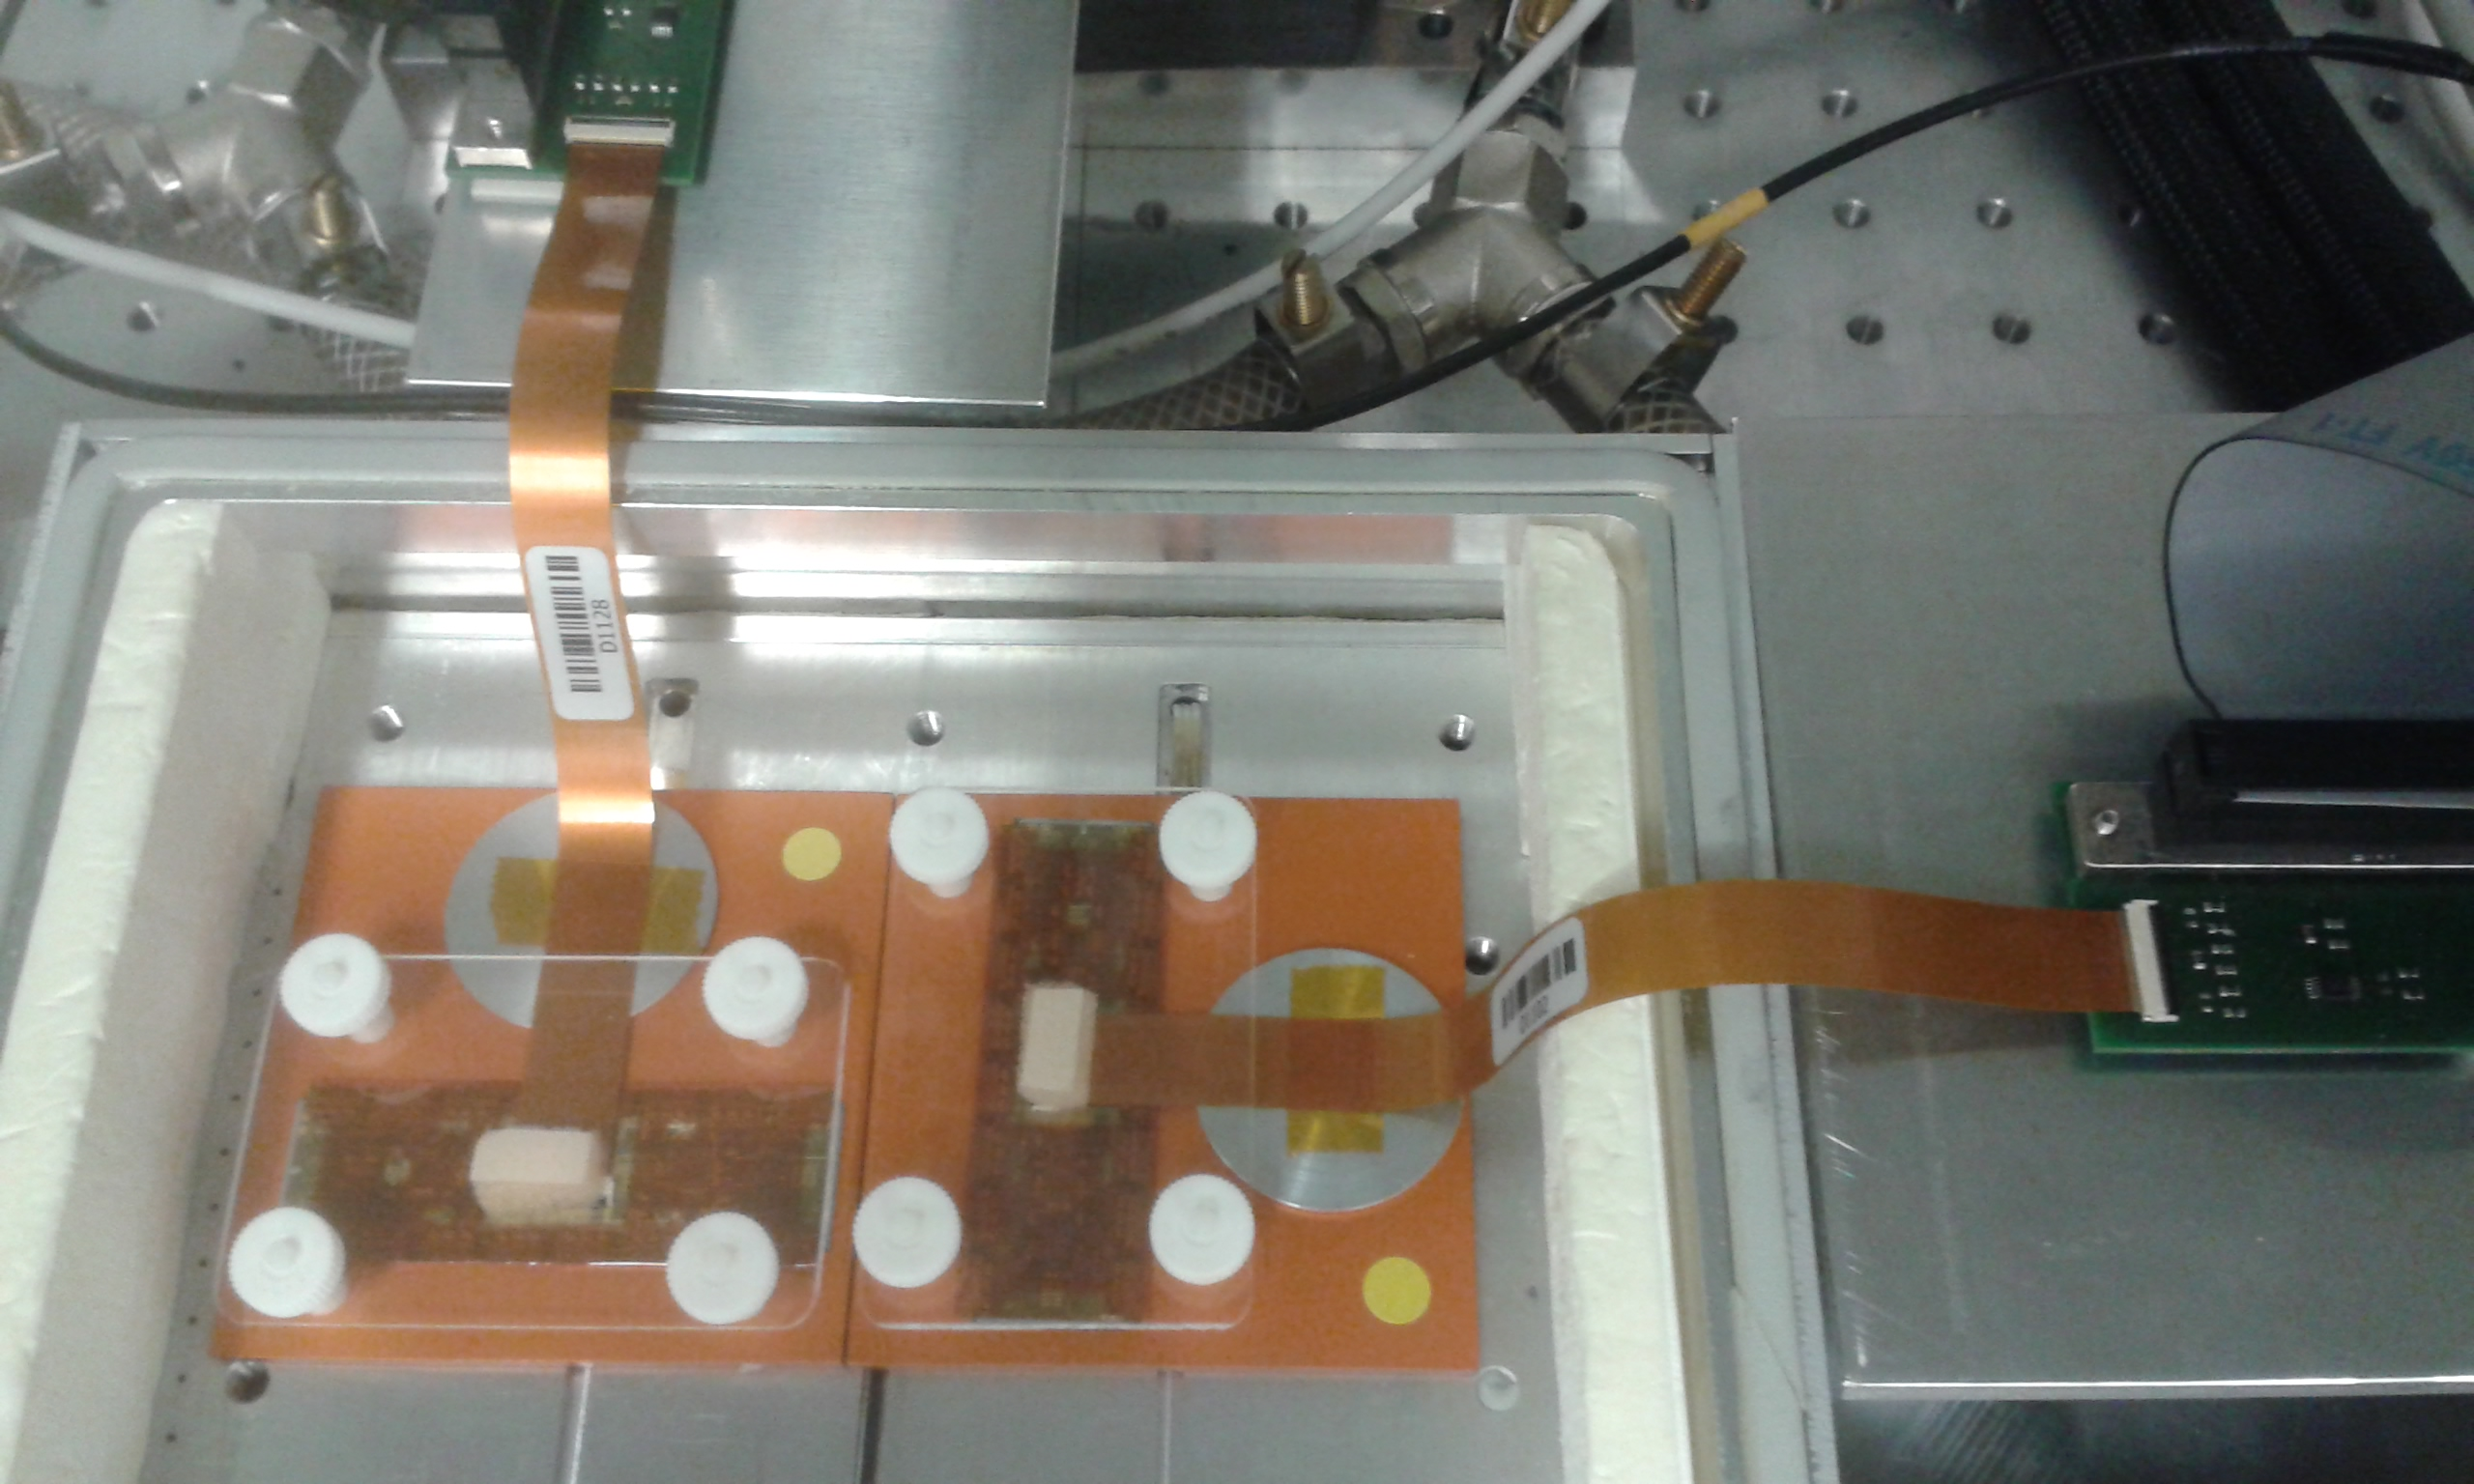
\includegraphics[width=\textwidth]{./L1test.jpg}
  \caption{\em Picture of the placement of two L1 modules in the climatic chamber}
  \label{L1test}
\end{minipage}%
\hspace{1mm}
\begin{minipage}{.49\textwidth}
  \centering
  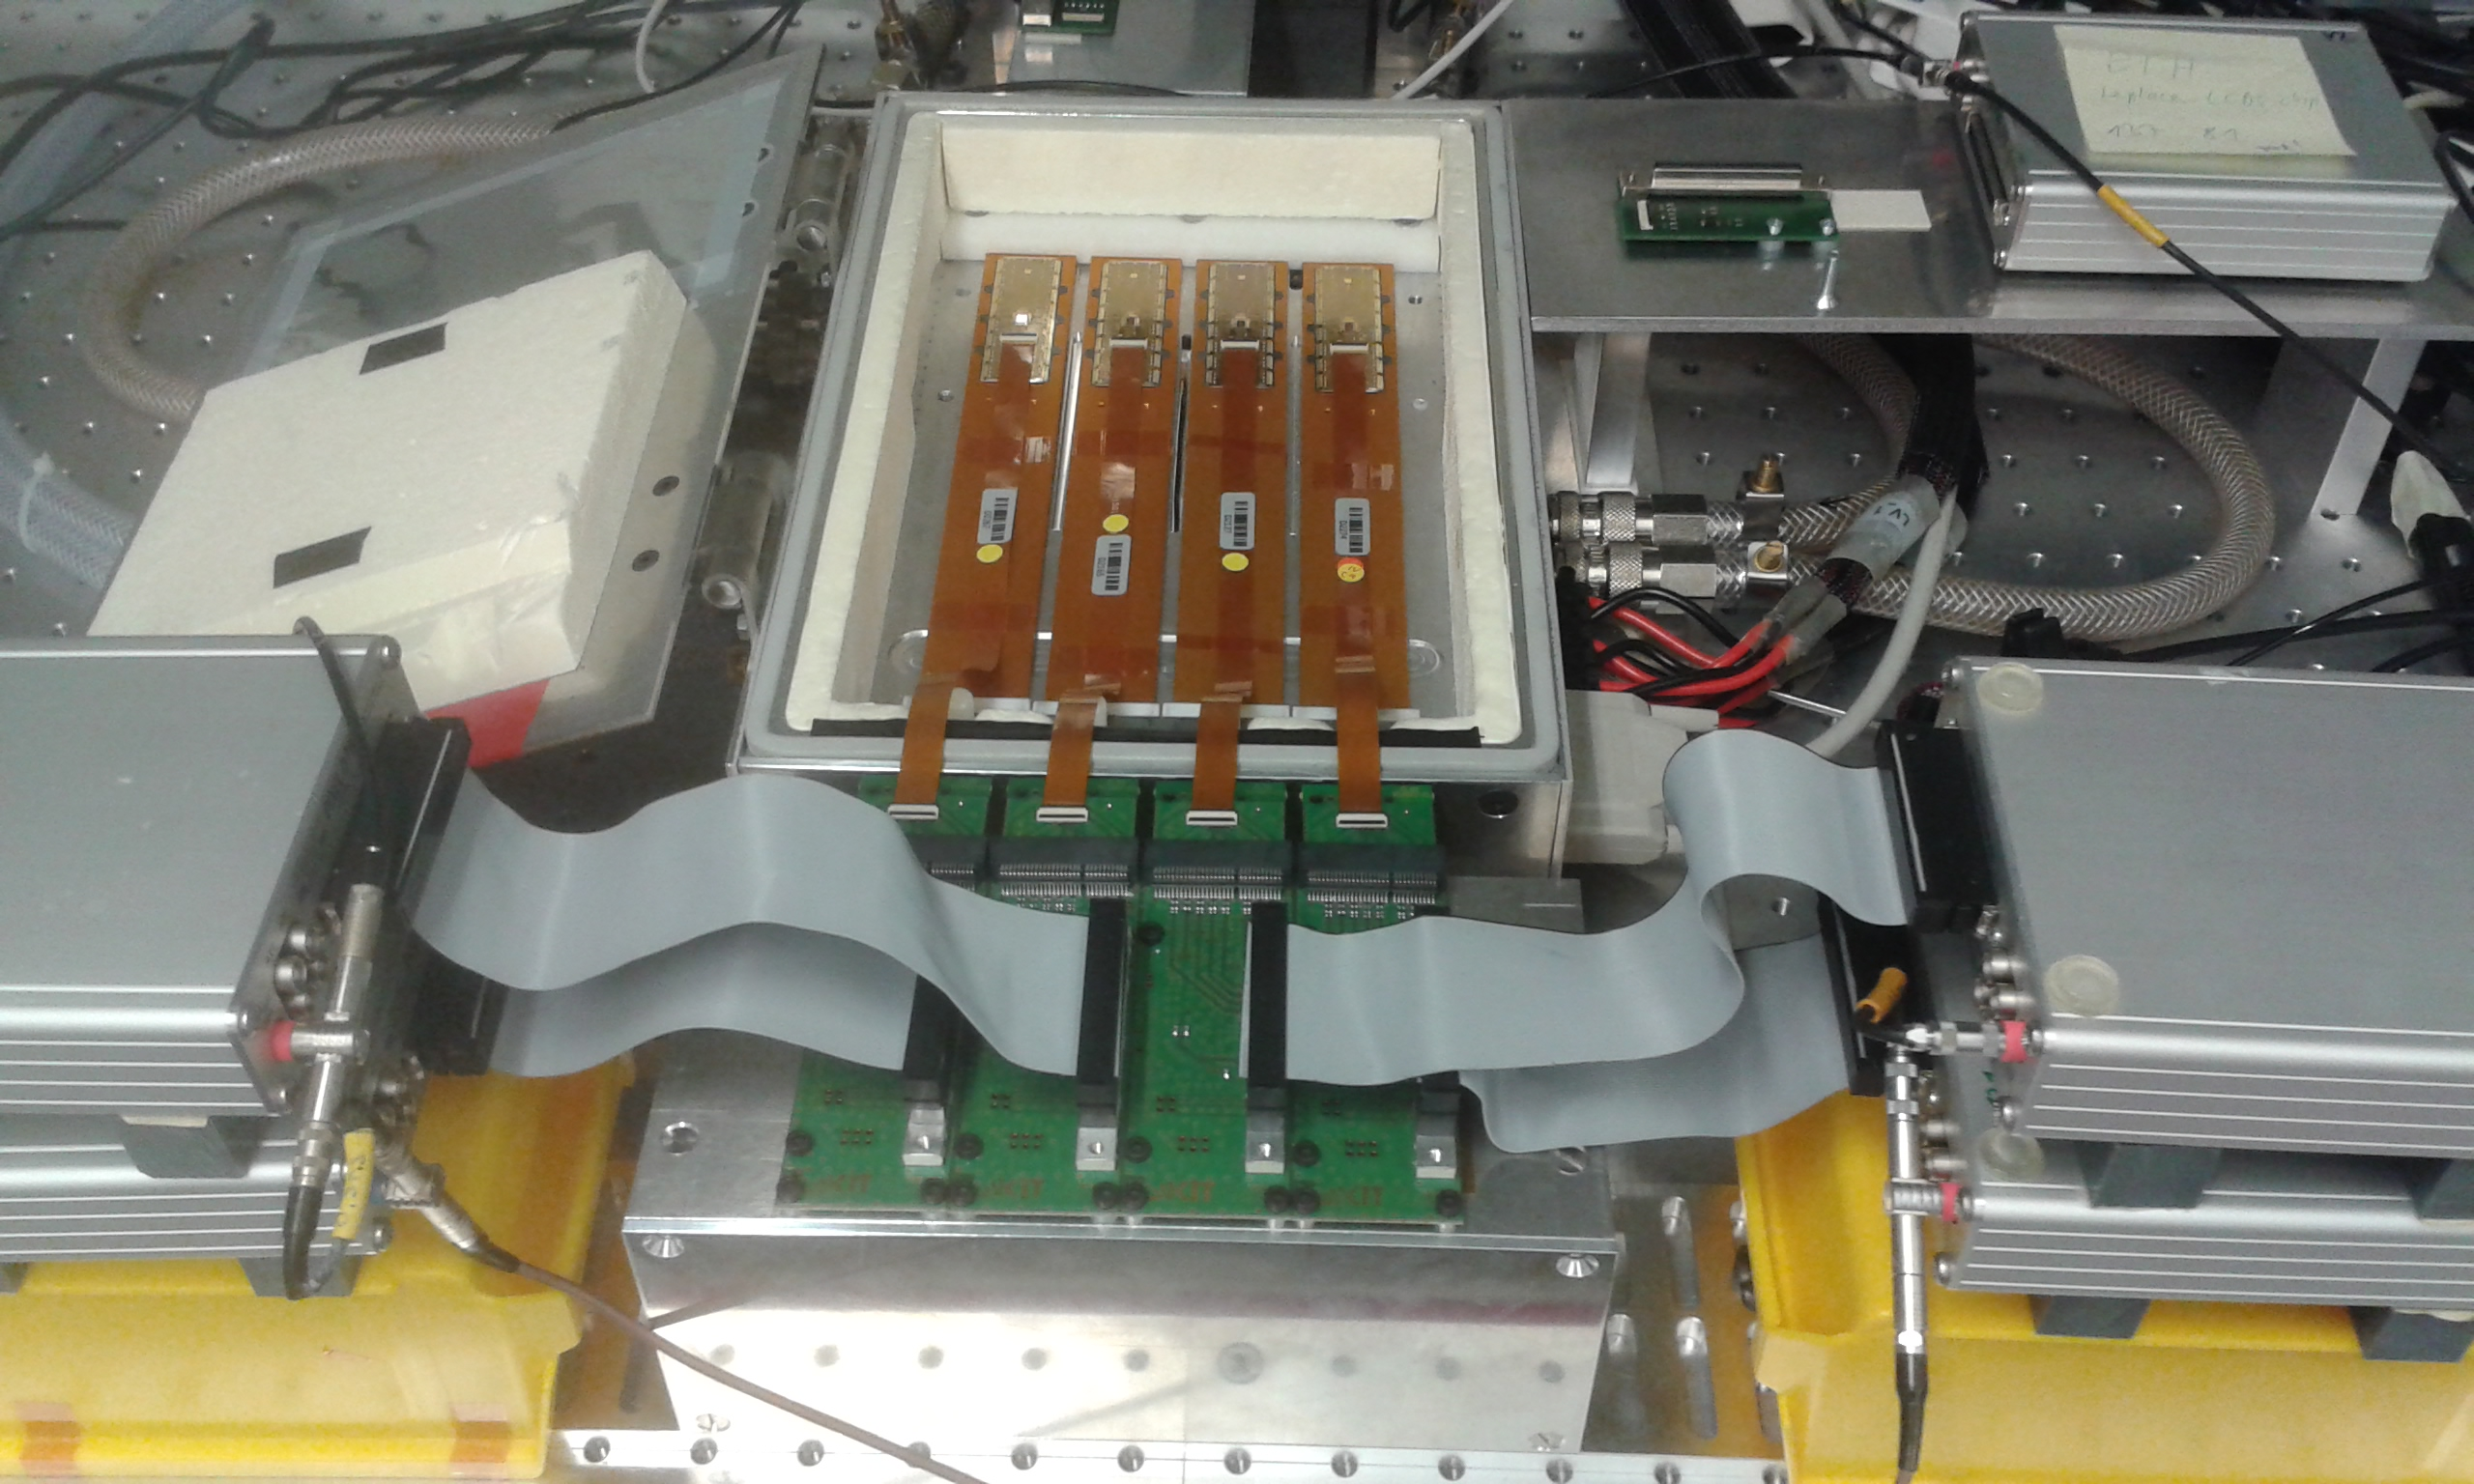
\includegraphics[width=\textwidth]{./L2test.jpg}
  \caption{\em Picture of the placement of four L2 modules in the climatic chamber}
  \label{L2test}
\end{minipage}
\end{figure}

Two L1 modules fit in the climatic chamber. Figure~\ref{L1test} shows their orientation.
Four L2 modules can be positioned with the available fixations in the climatic chamber as can be seen in Figure~\ref{L2test}.The modules need to be placed under the window covered with aluminium foil
Note that the modules should be placed underneath the window in the cover of the climatic chamber which is covered with aluminium foil. 

\section{Programs used for the qualification}

The testing of L1 and L2 has been almost completely automatized. This is performed by three different pieces of software. The tests are performed with \textbf{pXar}, \textbf{elCommandante} operates the different components of the set up and \textbf{MoReWeb} analyses the results of the qualification.

\subsection{elCommandante}

The testing is done automatically, meaning that a software called "ElCommandante" takes care of stirring all devices, including the power supply, the X-ray tube, the targets and the software executing the tests. Only the cooling has to be set manually


\subsection{pXar}
Pxar is the software which communicates with the modules. It needs as input DAC settings, trimbit settings and several configuration files for the modules and the tests.

\subsection{MoReWeb}

MoReWeb analyses the results of the X-ray qualification automatically and assigns a grade to every module.

\section{Specific testing conditions for L1 modules}

L1 modules have several problems that prevents using the same qualification procedure than for L2 modules. Since the power consumption of L1 modules is excessively high leading to many read-out errors at low thresholds, the modules are tested at a threshold of Vcal 80 (4000 e$^-$) instead of 35 (1500 e$^-$). 

The noise of the PROC600V2 is quite high when all pixels are unmasked and when exposed to radiation, in particular for the edge and corner pixels, which size is twice or four times the usual pixel size. This is why the two corner pixels 0,79 and 51,79 are masked for every ROC. Otherwise, the high noise of those pixels handicaps the entire readout of the ROC. In addition to this, the threshold of all other edge pixels is increased even further than the 80 Vcals. Furthermore, no grading on the noise of L1 modules is applied.

Due to this high threshold and because the ADC response of the pulse hight is not stable under rate, the Vcal Calibration is not performed for the modules. 
It would be possible to get an approximative calibration by trimming the module to a lower threshold and masking every second row and every second column to limit the noise. Then, the PH calibration algorithm would have to be rewritten such that it takes into account the jumps in the ADC. This jump is more important for uneven rows, so it is recommended to mask those.


\section{Performing the X-ray qualification}

This section describes the steps of an X-ray qualification, from the setting up of all needed configuration files to the handling of the devices. 

\subsection{Starting the X-ray qualification}

\subsubsection{Start the necessary devices}

\begin{itemize}
\item Put the modules to be tested (up to 4 L2 or 2 L1 modules) in the X-ray set up as described above.
\item Execute points 1 to 5 from Section~\ref{Xraysetup}.
\item Turn on Keithley (only button 1).
\item Turn on climatic chamber and set the cooling to 17$^{\circ}$.
\item Verify that all DTBs are powered.
\end{itemize}

\subsubsection{Set-up directory for start parameters}

In order to start the qualification, pxar needs configuration parameters for the module. These can be copied from the \testname{FullTest}@17 from the FQ. With these, it is not necessary to trim the module again and to optimize its pulse height which saves time.

To prevent having too large files containing the results of the qualification, one can remove unneeded .root and .log files from the FQ. For instance, one can use the script \textbf{python ./clean\_parameters\_folder.py -d Mxxx} which is located in the home directory of the \textit{production} user. Mxxx designates the module name. \\

Examples for the elCommandante.ini and elCommandante.conf files for L1 and L2 module qualification can be found in Appendix~\ref{Config}.

\subsubsection{elComandante configuration}

\begin{itemize}
\item Two different versions of elComandante are used for module configuration such that the configuration files do not have to be changed every time for the FQ and the X-ray qualification. Therefore, use the elCommandante version:  \textbf{/home/production/elComandante{\color{Red} Xray}/}
\item Check the elCommandante.ini and elCommandante.conf files located in the \textbf{/home/production/elComandante{\color{Red} Xray}/config} directory. In particular, verify the test chain in the elCommandante.ini file. This differs for the qualification of L1 and L2 modules. For L2 modules, the test chain should be:

\begin{Verbatim}[frame=single]
[Tests]
Test = PixelAlive@17>GainPedestal@17>RetrimHotPixels@150MHz/cm2>
{HRData@50MHz/cm2,HRData@150MHz/cm2,HRSCurves@100MHz/cm2,
XraySpectrum@Zn,XraySpectrum@Mo,XraySpectrum@Ag,XraySpectrum@Sn,
CalDelScanAndSaveDacs@4mA25kV>{HREfficiency@50MHz/cm2,
HREfficiency@100MHz/cm2,HREfficiency@150MHz/cm2,
HREfficiency@200MHz/cm2,HREfficiency@250MHz/cm2}}
TestDescription = XrayQualification
\end{Verbatim}

and for L1:

\begin{Verbatim}[frame=single]
[Tests]
Test = PixelAlive@17>IncreaseEdgeThr@17>
RetrimHotPixels@150MHz/cm2>RetrimHotPixels@50MHz/cm2>{
HRData@100MHz/cm2,HRData@300MHz/cm2,HRSCurves@250MHz/cm2,
CalDelScanAndSaveDacs@100MHz/cm2>{HREfficiency@50MHz/cm2,
HREfficiency@100MHz/cm2,HREfficiency@150MHz/cm2,
HREfficiency@200MHz/cm2,HREfficiency@250MHz/cm2,
HREfficiency@300MHz/cm2,HREfficiency@400MHz/cm2}}
TestDescription = XrayQualification
\end{Verbatim}

Note that the names of the tests are not the same than the corresponding names in pxar for those tests. This is due to the fact that some modifications are applied to some of those tests in the qualification, such as delays before their execution or saving the acquired DACs. These modifications do not alter the outcome of the tests. 
Table~\ref{tests} shows which pxar test is executed for each test in the test chain.


\begin{table}[]
\centering
\caption{Correspondence between test names in ElCommandante and in pxar}
\label{tests}
\begin{tabular}{@{}lll@{}}
\toprule
ElCommandante test    & pxar test                & Modifications               \\ \midrule
RetrimHotPixel        & trimhotpixels            & 5s delay before test        \\
HRData                & phrun                    & 5s delay before test        \\
HRSCurves             & xnoisemaps\footnotemark             &                             \\
XraySpectrum          & phrun                    & 30s delay before test       \\
CalDelScanAndSaveDacs & caldelscan\footnotemark[\value{footnote}]               & Save DACs after test        \\
HREfficiency          & pixelalive + xpixelalive\footnotemark[\value{footnote}] & 1s delay between both tests \\
IncreaseEdgeThr       & incedgethr               &                             \\ \bottomrule
\end{tabular}
\end{table}

\footnotetext{Please note that these tests are implemented differently for L1 and L2 module tests. The test procedure remains the same for both types of modules. Tests for L1 modules are found in the XPixelAlive2 tab of pxar and for L2 in the HighRate one. Make necessary modifications in the ./ElCommandanteXray/config/tests/ files.} 


Furthermore, note that one can specify the testing conditions in these test chains, such as the target used for the XraySpectrum tests and the X-ray hit rate which reflects in different tube settings.



\end{itemize}
\subsubsection{Starting the qualification}

\begin{itemize}
\item Use elComandante from \textbf{/home/production/elComandante{\color{Red} Xray}/elComandante}
\item Run ./el\_comandante.py
\item Scan modules with scanner from left to right, press enter for an empty position or if the module is the same than in the previous test. Otherwise, the module names can also be inserted manually in the elCommandante.ini file.
\end{itemize}


\subsection{Finishing the qualification}

\subsubsection{Analysing the data}

These steps summarize the actions needed to finish the X-ray qualification. Steps 4-6 are not necessary but were performed during the 2015-2016 production to keep a good overview of all test results.

\begin{itemize}
\item Check the test list in the elComandante output (below "Final cleanup after all tests ..."). The status code should always be 1. A status code of $\neq 1$ or a red color means that a test has failed. 
\item Copy files from local directory (eg. /usr/local/data/) to a location where all test results are kept. Copying .tar files and extracting them is faster than copying the full uncompressed directory. 
\item Analyze the tests with MoReWeb.
\item Update MoReWeb overview on the groups webserver. For this, use the script \textbf{/home/production/ synchronize\_webserver.sh}. This might need to be adapted.
\item Write an Elog entry with the results of the qualification
\item Upload results to the Pisa database as follows:
\end{itemize}

\begin{Verbatim}[frame=single]
scp -P 23481 -i /data/Equipment/labcomputer/eth-pisa-key.rsa
 M1148_Full....tar eth@cmspixelprod.pi.infn.it:/home/eth/dropbox/
\end{Verbatim}

\subsubsection{Switching off the set-up}

\begin{itemize}
\item Remove modules from the climatic chamber and store them in a safe place.
\item Switch off the DTBs, the climatic chamber and the Keithley.
\item Perform the last four steps in Section~\ref{Operation} to switch off the Xray tube.
\end{itemize}

\subsection{Troubleshooting}

\prob{The DTBs are not detected by the computer, typical error message: Unable to detach testboard. USBview is very slow and might or might not list all connected DTBs}
\sol{Run the script \textbf{/home/production/reset\_usb.sh} (as root) or restart computer (only after agreement from the group).}
\prob{Hot Pixel Re-trimming takes very long or finds more hot pixels than usual}
\sol{Might be missing HV or wrong testParameters.dat file (for instance from an old pXar version).}
\prob{The Keithley is not turned on by elComandante}
\sol{Check if the \textbf{port} option in section \textbf{keithleyClient} in \textbf{elComandante.conf} is pointing to the correct device. Find the device by running the command \mbox{\textbf{findkeithley}} on production user. This device number can reset after reboot!}

\section{Description of the tests performed during the X-ray qualification}
\subsection{Module parametrization}
At the very beginning of the X-ray qualification, two tests of the Full Qualification are repeated. 
\begin{itemize}
\item PixelAlive: Since the module is handled between both qualifications, a PixelAlive test is performed as a quick verification that no major damage occurred during the handling.
\item GainPedestal: The calibration between PH in ADC units and in Vcal units is also repeated since it is very sensitive to environmental features such as temperature which can change slightly between the set up of the FQ and of the X-ray qualification. It is important that this calibration is accurate as it is used for the Vcal Calibration which will be described later. Since the Vcal calibration is not performed for L1 modules, the GainPedestal test is also omitted for L1 modules.
\end{itemize}
\subsection{IncreaseEdgeThr - only for L1 modules}
\subsubsection{Purpose}
It is known that the corner pixels and edge pixels are much noisier that the inner ones on the PROC600V2. This is why the threshold of those pixels is further increased during before performing tests during which all pixels are enabled.
\subsubsection{Methodology}
This test only affects the edge pixels. The trim bit of those pixels are either increased by 8, or set to 15 if the resulting trim bit would be higher than 15. In addition, the trim bit of the corner pixels is automatically set to 15.
\subsubsection{Output}
This test does not produce any output.
\\
\\
All subsequent tests are performed under X-ray radiation.
\subsection{Trimhotpixels}
\subsubsection{Purpose}
Some pixels become very noisy when the module is exposed to radiation. This is why in this test, noisy pixels are identified and their threshold increased or the pixel masked if the maximum trimbit has been reached.
\subsubsection{Methodology}
During this test, the module is exposed to radiation. Hits are accumulated for a given time and a hit map is acquired. After this, the measured hit rate in each pixel is evaluated and compared to a threshold rate which is set. If the measured rate is higher than that threshold, the trimbit of that pixel is increased by one and the test is repeated either until the pixel is not crossing the threshold any more or until the trimbit value has reached 15. In this case, the pixel is flagged as noisy and masked. 
It is accounted for the different size of the edge pixels in the comparison of the measured rate and the threshold rate.
\subsubsection{Output}
Figure \ref{RetrimHotPixels-Hitmap} shows the hit map that was acquired. The pixel colored in red has a X-ray hit rate which is higher than the set threshold and is therefore retrimmed. Figure~\ref{RetrimHotPixels-TrimbitHitmap} confirms that the trim bit value of this pixel has been increased by 8.
\begin{figure}
\centering
\begin{minipage}{.48\textwidth}
  \centering
  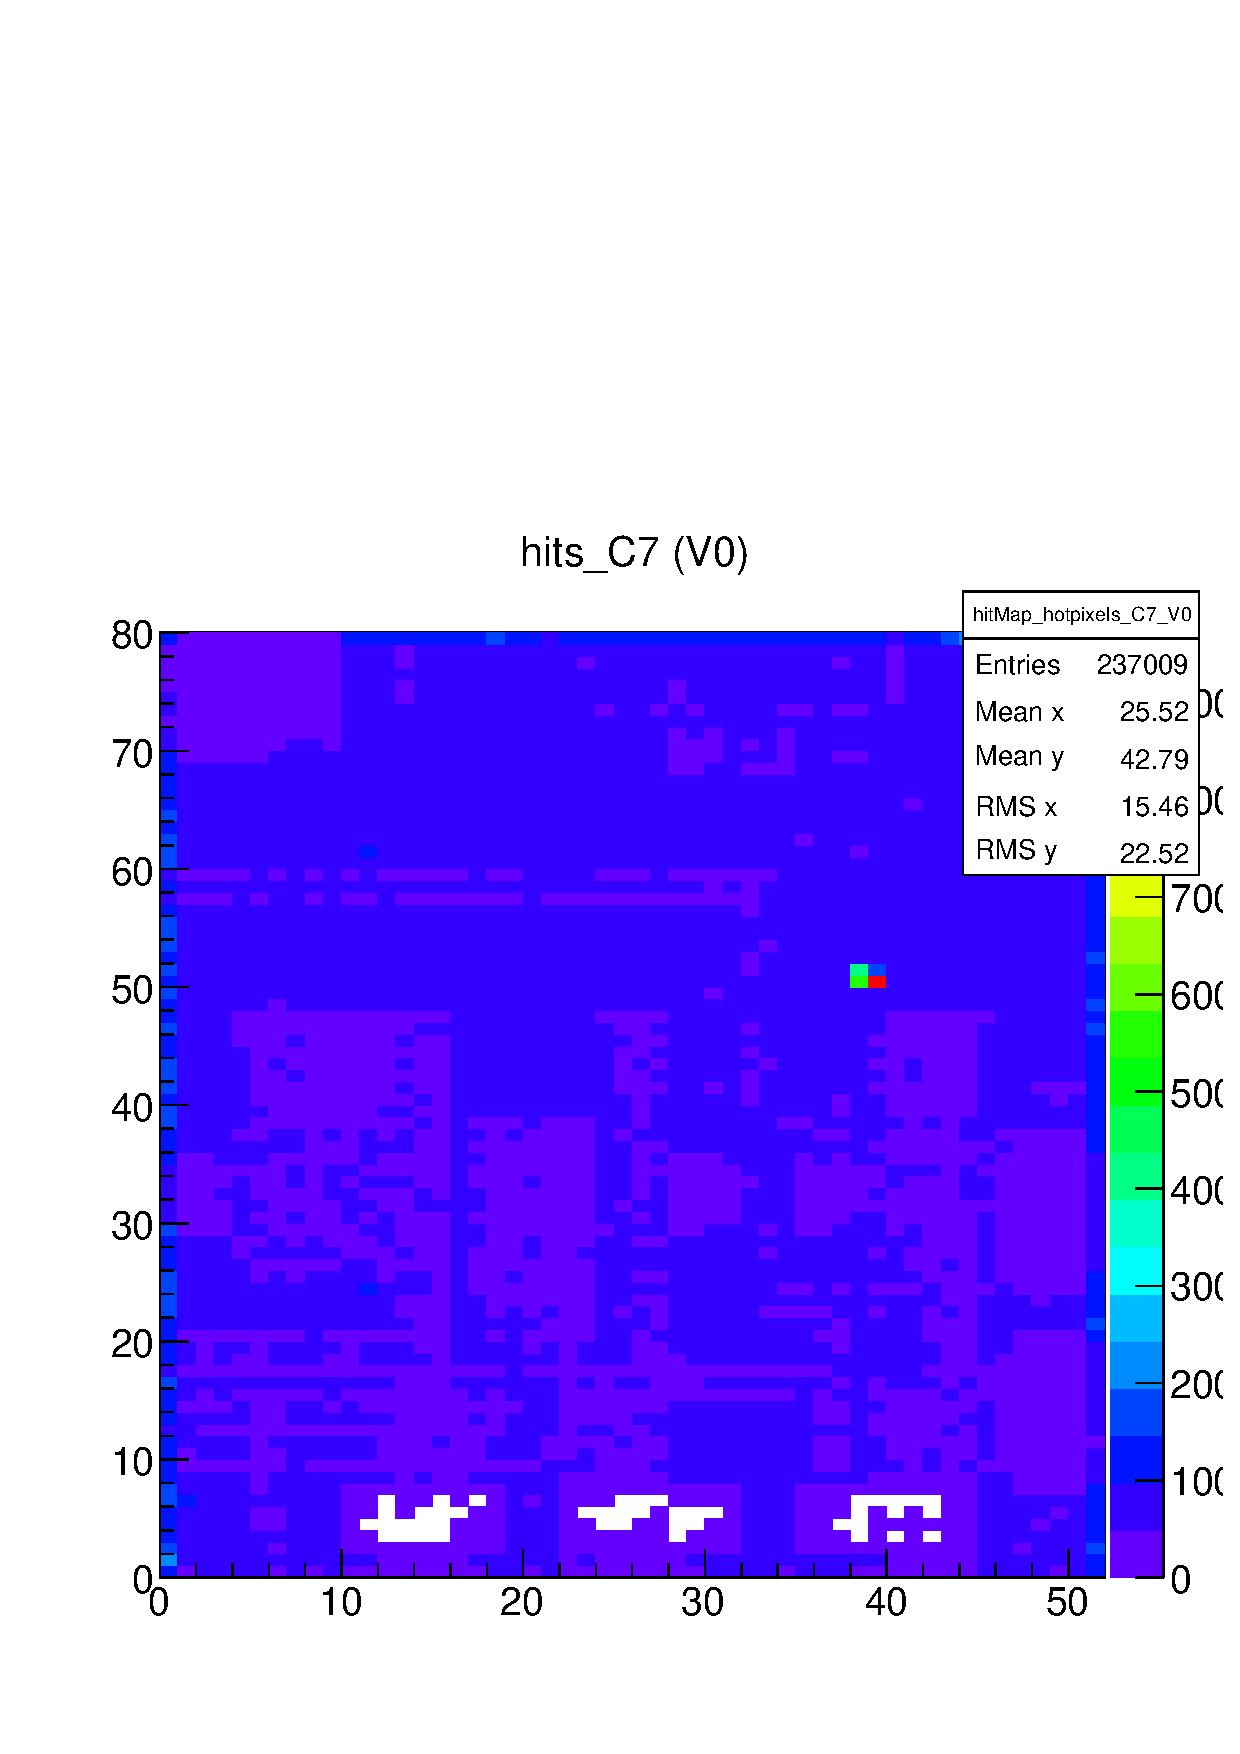
\includegraphics[width=\textwidth]{./RetrimHotPixels_Map.pdf}
  \captionof{figure}{ROC map of the number of hits acquired per pixel \\}
  \label{RetrimHotPixels-Hitmap}
\end{minipage}%
\hspace{2mm}
\begin{minipage}{.48\textwidth}
  \centering
  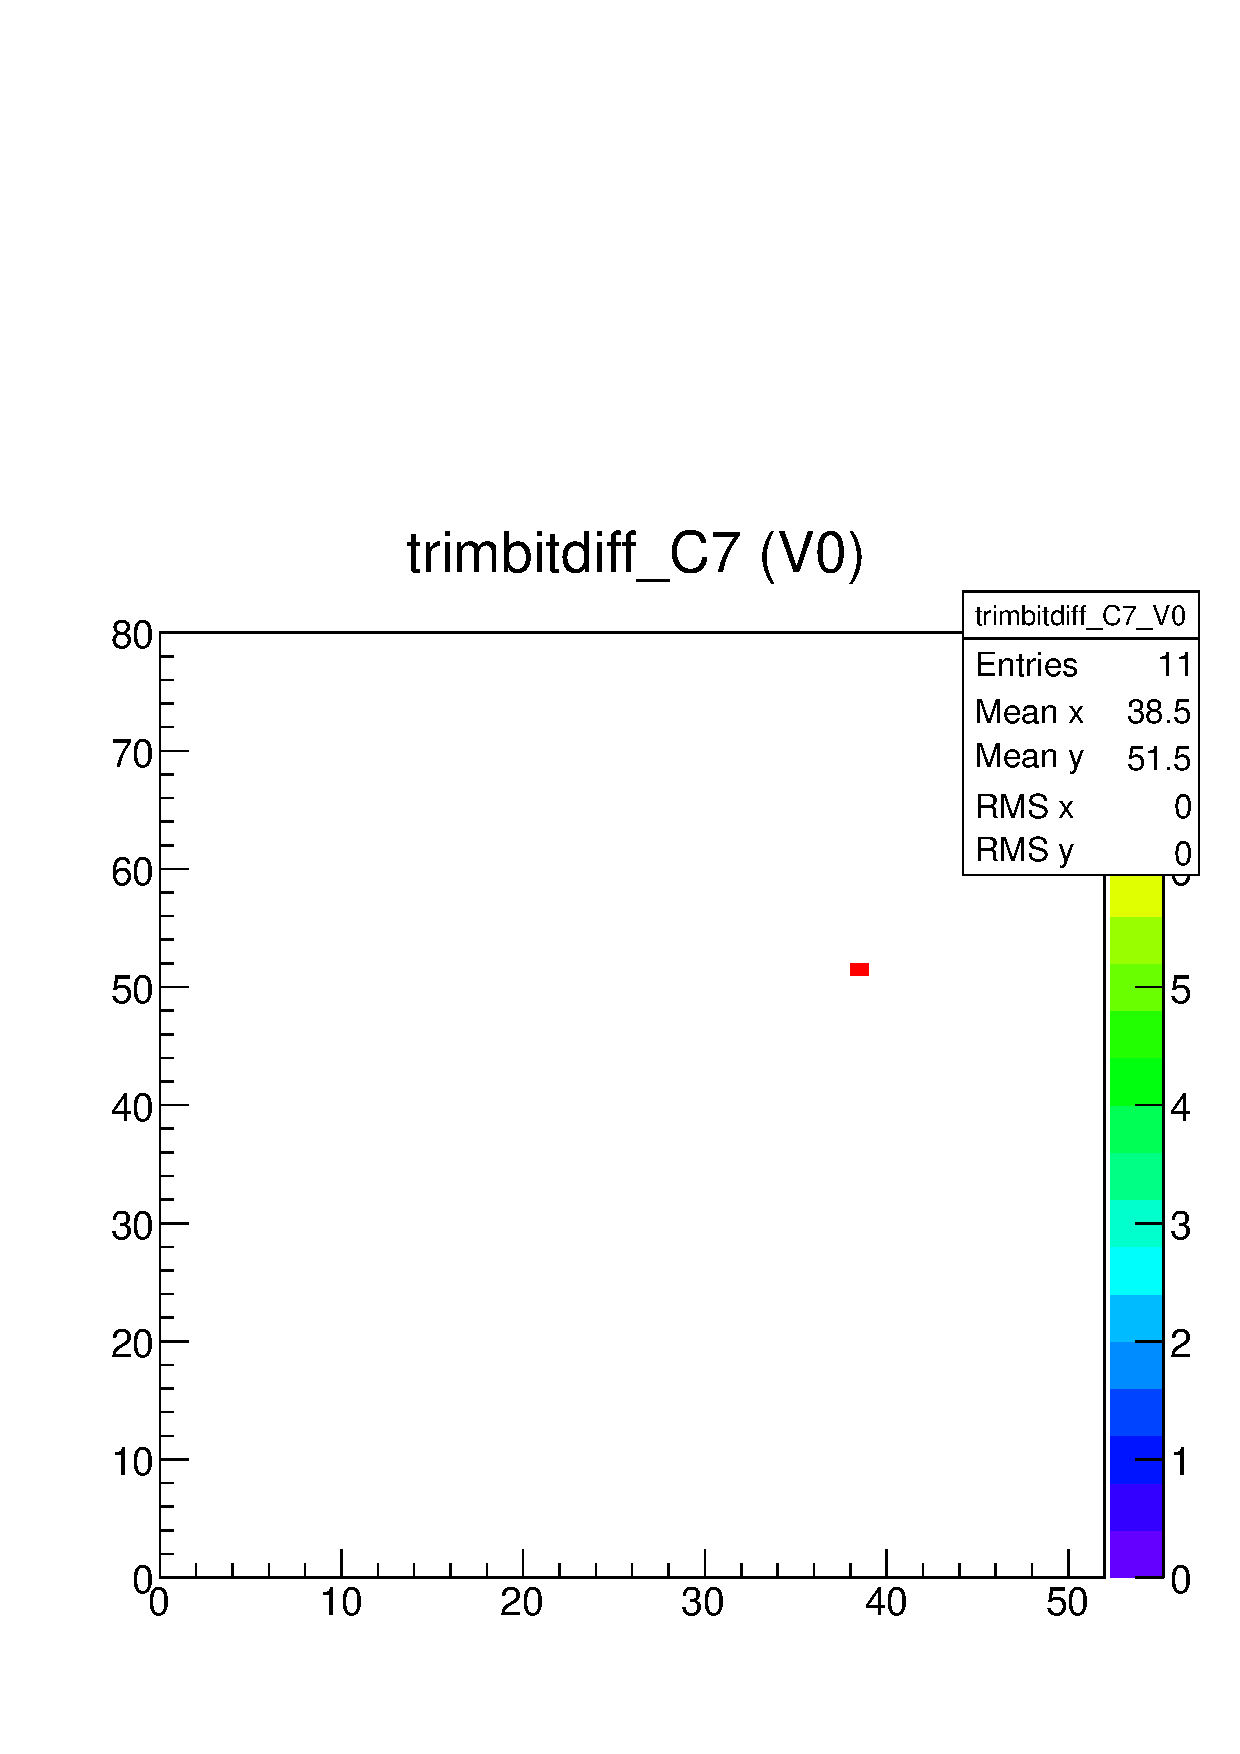
\includegraphics[width=\textwidth]{./RetrimHotPixels_TrimBitDiff.pdf}
  \captionof{figure}{ROC map showing the difference between the original trimbit value and the value set after the test}
  \label{RetrimHotPixels-TrimbitHitmap}
\end{minipage}
\end{figure}

\subsection{PHrun}
\subsubsection{Purpose}
This test aims to verify the readout uniformity of each double column of the module by verifying if the measured hit rate increases as expected with higher X-ray rates and also if the readout is stable over time.
\subsubsection{Methodology}
This test has all pixels enabled at the same time and acquired a hit map of all incoming X-rays. To prevent the buffers to data and timestamp buffers to overflow which can happen at higher X-ray rates, data acquisition is stopped whenever more than 70\% of the buffers are occupied. Data acquisition is resumed once the data in those buffers has been read out.
\subsubsection{Output}

Figures~\ref{HRData-PHmap} to \ref{HRData-HitsEventColumn} show the output of the HRData test. Figure \ref{HRData-PHmap} shows the average pulse height of all hits in a double column. Ideally there should not be any visible structure. Figure~\ref{HRData-PHHisto} histograms the pulse height of all recorded X-ray hits in all pixels. Figure~\ref{HRData-Qmap} shows again the average pulse height of all hits per pixel, but the pulse height here is converted to Vcal units. The pulse height of every hit in Vcal units is shown in Figure~\ref{HRData-Qhisto}. Figure~\ref{HRData-Hitmap} shows the amount of X-ray hits per pixel. The read-out uniformity over time is verified in Figure~\ref{HRData-HitsEvent}. One events regroups all hits detected between two triggers, which come every \SI{100}{\kilo\hertz}. This line should therefore be as flat as possible. Figure~\ref{HRData-HitsColumn} shows the number of hits per column. The first and last column is expected to have about twice the number of hits than the other columns since the pixel size of those columns is larger. Otherwise, the number of hits should be similar for all columns, though there can be some fluctuations due to the structure of the HDI which shields some parts of the module more than others. Figure~\ref{HRData-HitsEventColumn} summarizes the information from the two last plots.

\begin{figure} [h!]
\centering
\begin{minipage}{.48\textwidth}
  \centering
  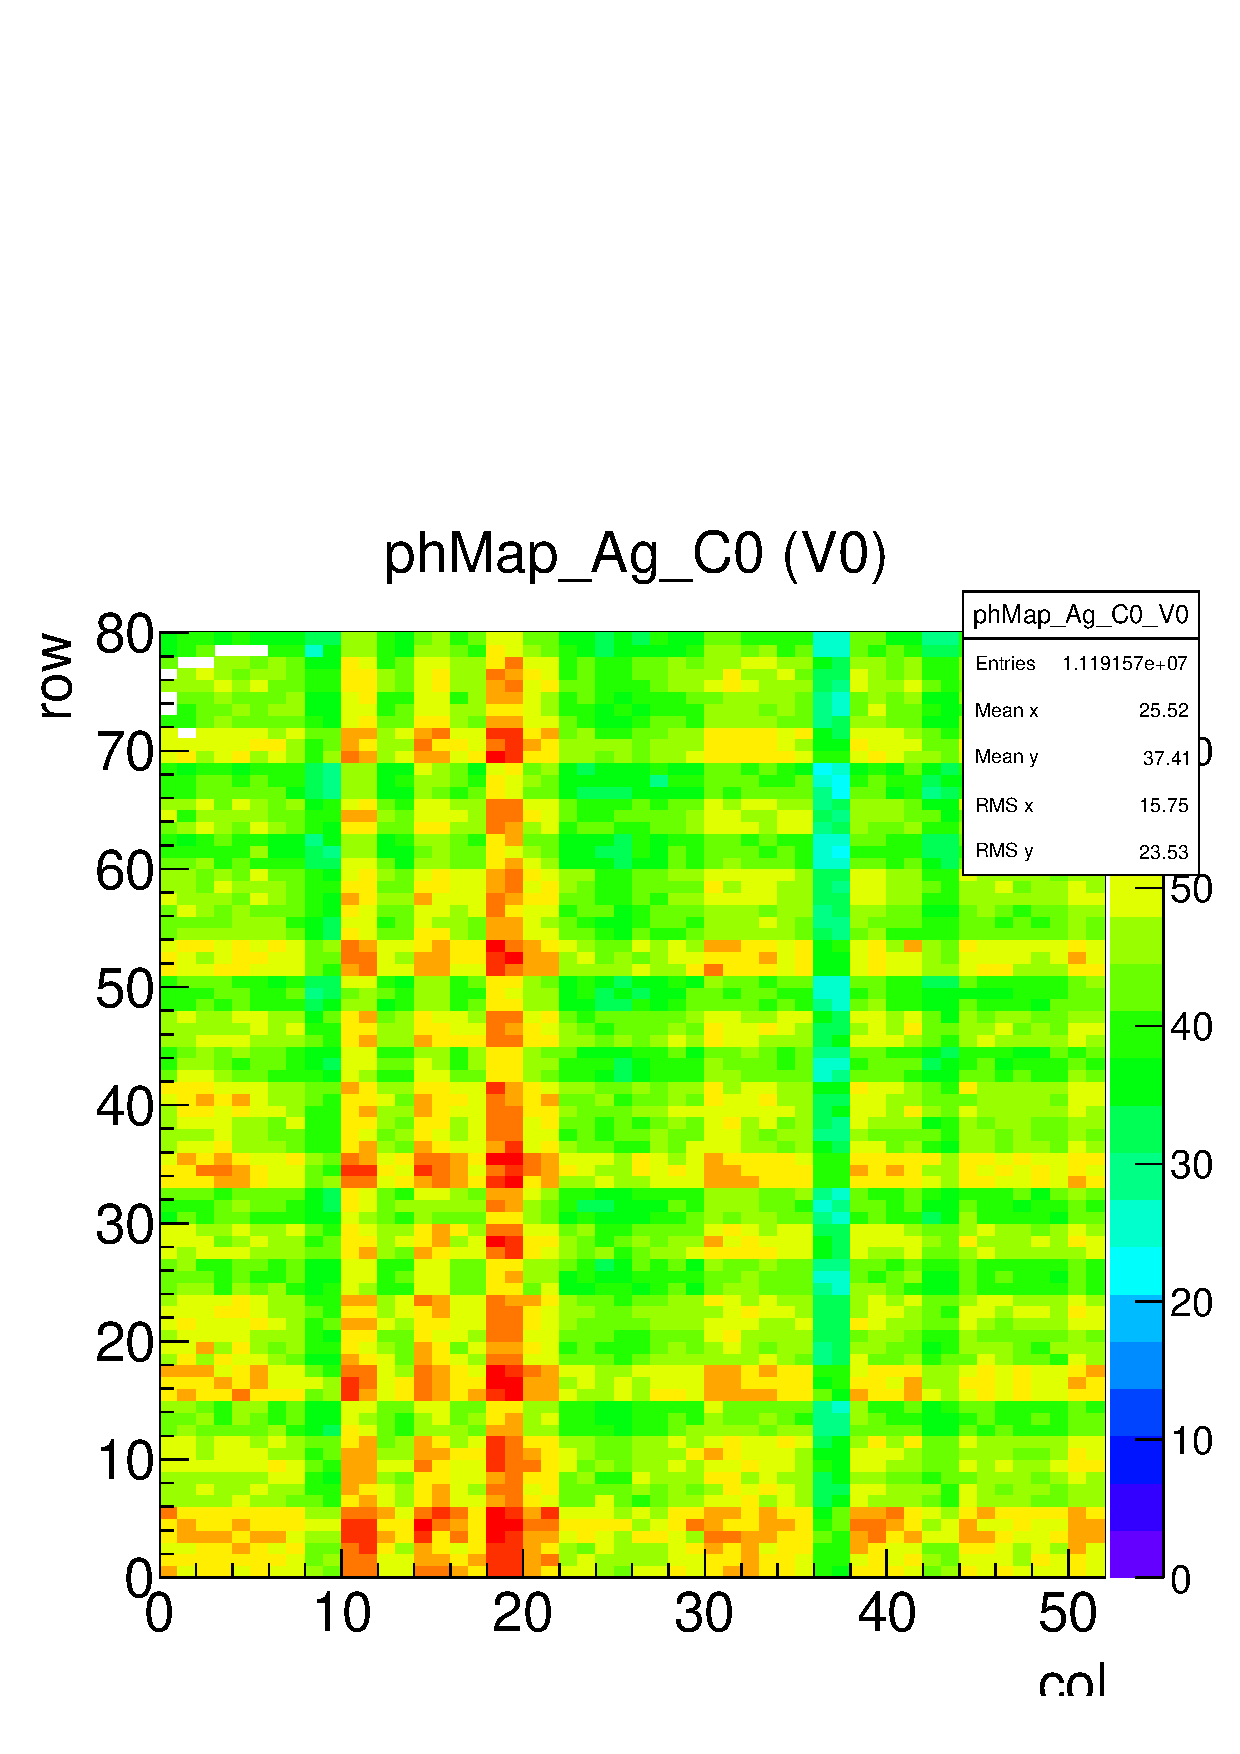
\includegraphics[width=\textwidth]{./HRData_PHMap.pdf}
  \captionof{figure}{ROC map of the average pulse height of all hits in each pixel}
  \label{HRData-PHmap}
\end{minipage}%
\hspace{2mm}
\begin{minipage}{.48\textwidth}
  \centering
  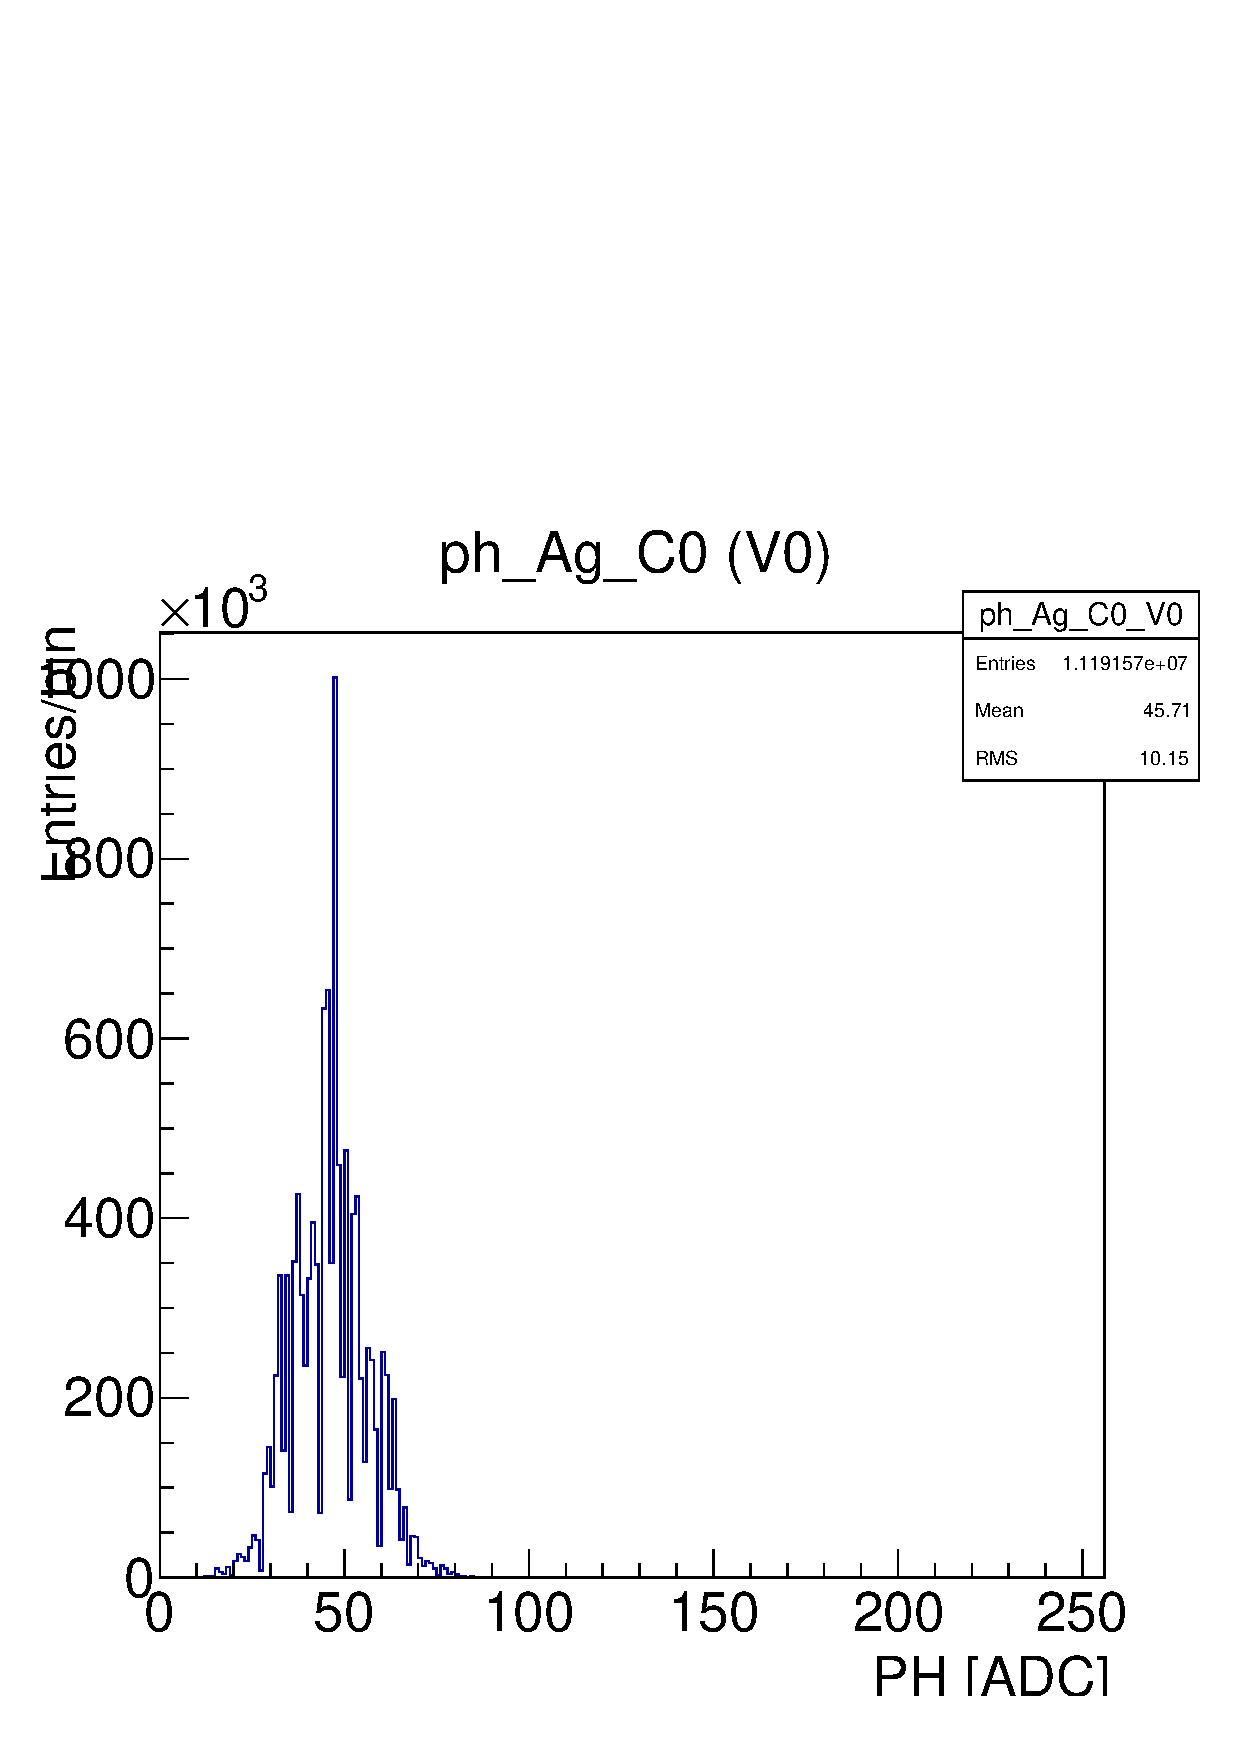
\includegraphics[width=\textwidth]{./HRData_ph_histo.pdf}
  \captionof{figure}{Histogram of the pulse height of every hit recorded by one ROC}
  \label{HRData-PHHisto}
\end{minipage}
\end{figure}

\begin{figure} [h!] 
\centering
\begin{minipage}{.48\textwidth}
  \centering
  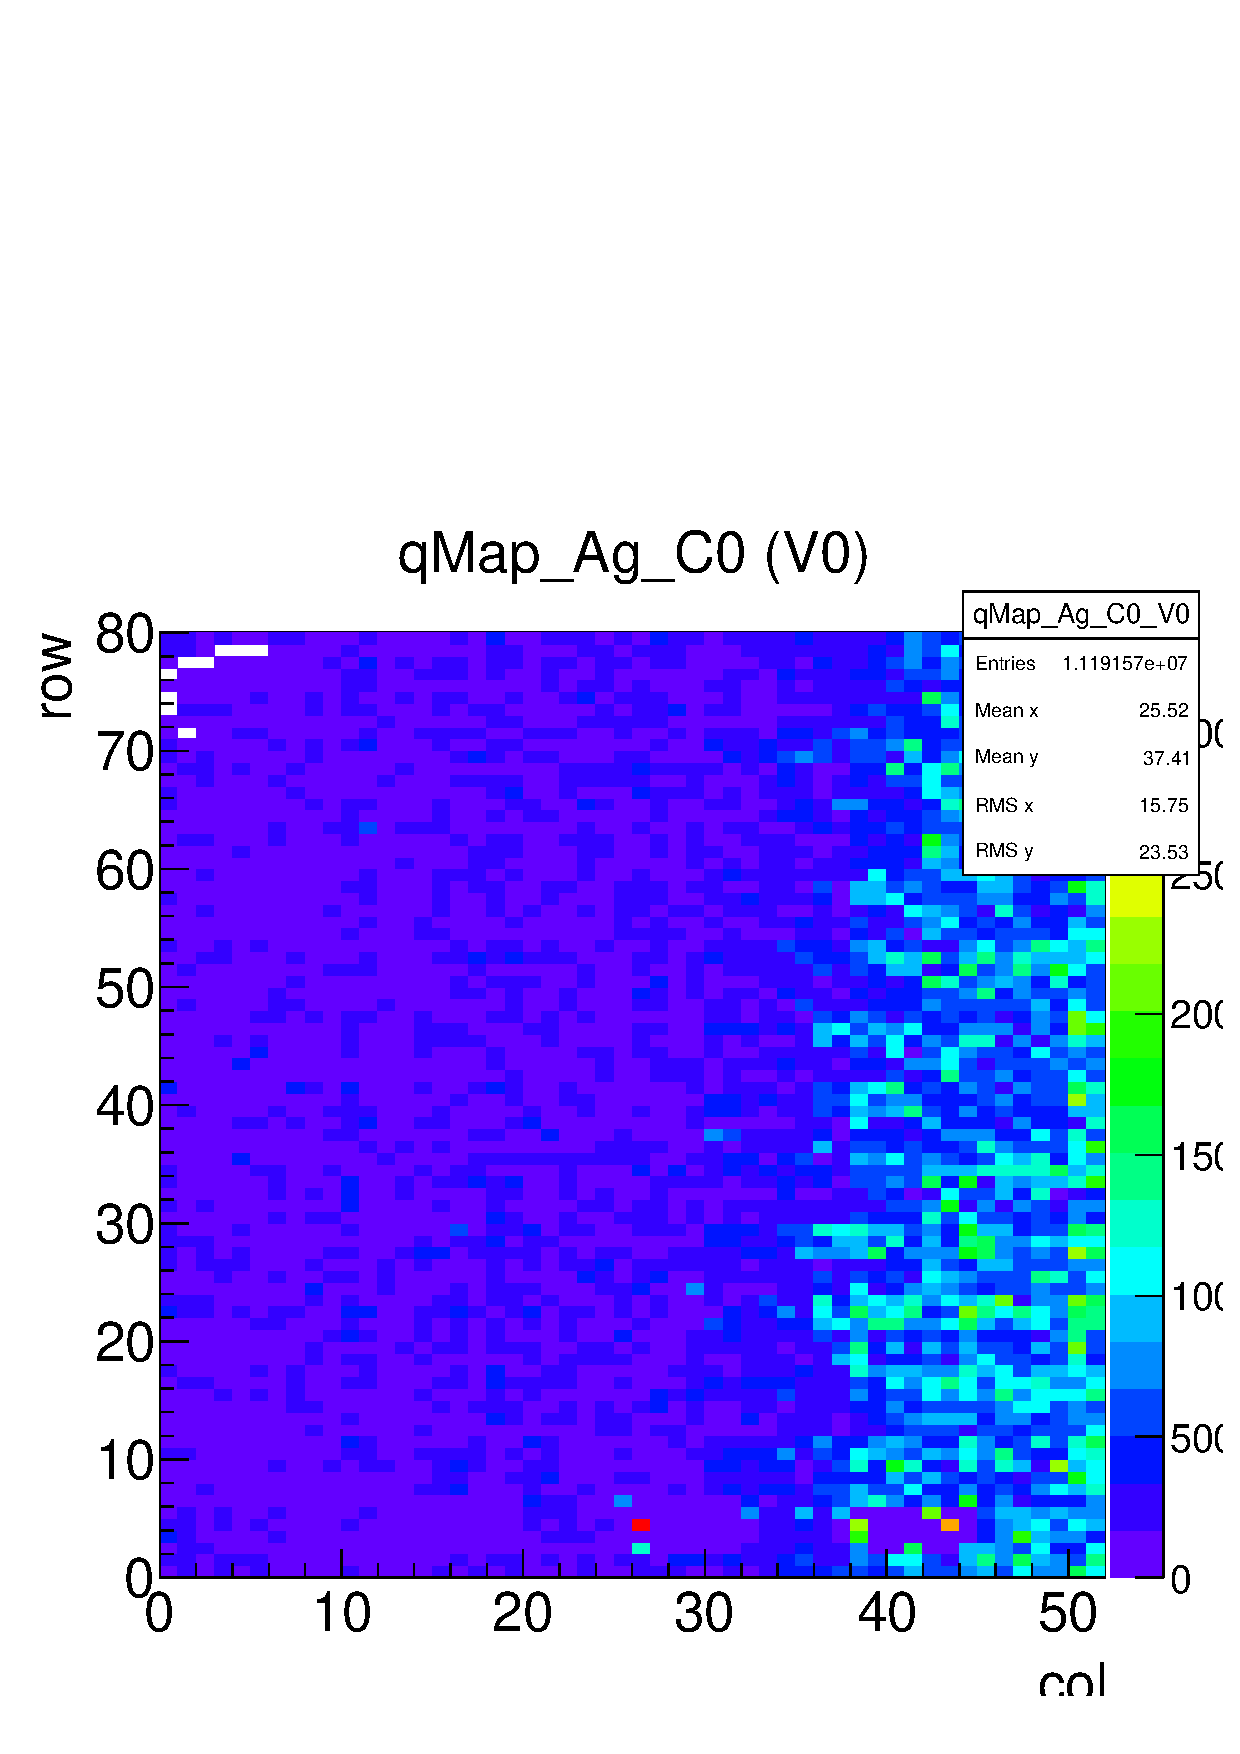
\includegraphics[width=\textwidth]{./HRData_qMap.pdf}
   \captionof{figure}{ROC map of the converted average pulse height in Vcal units }
  \label{HRData-Qmap}
\end{minipage}%
\hspace{2mm}
\begin{minipage}{.48\textwidth}
  \centering
  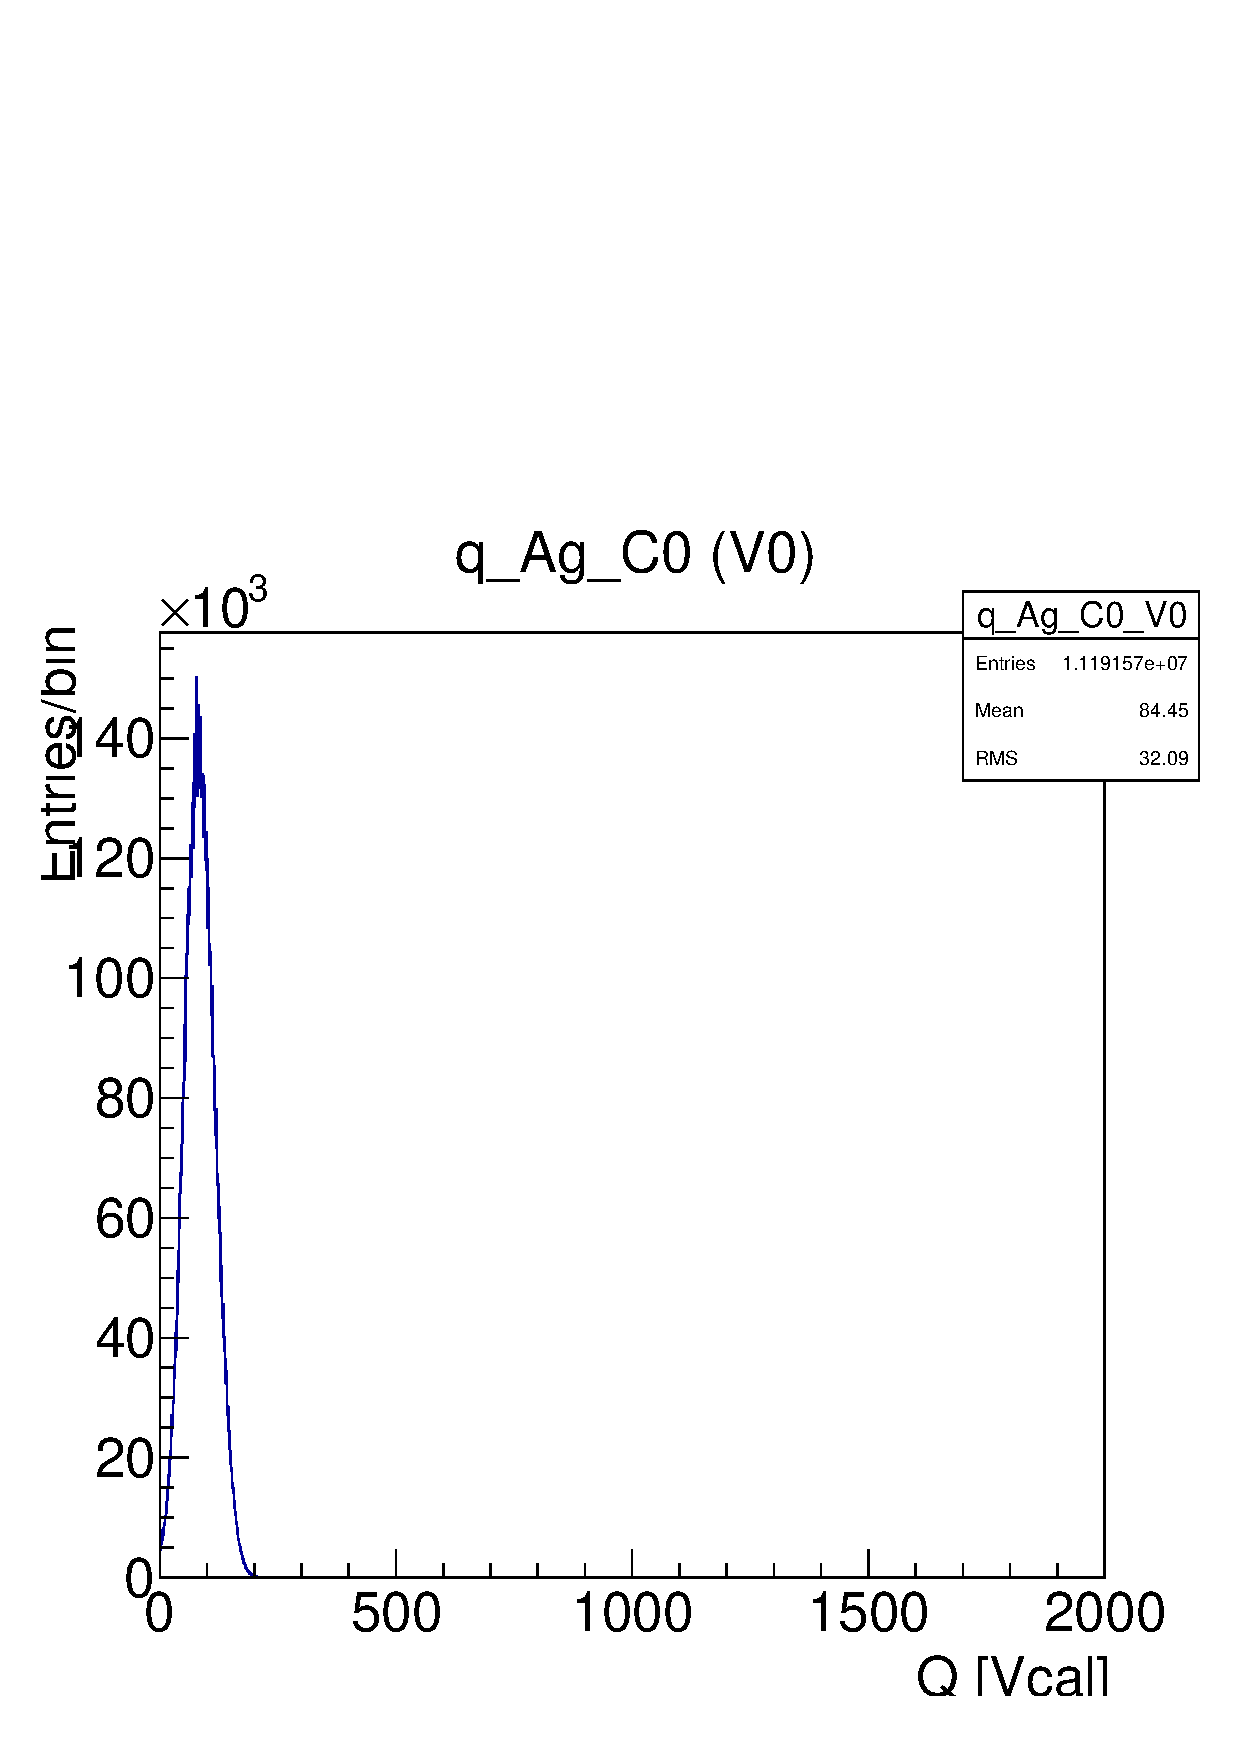
\includegraphics[width=\textwidth]{./HRData_q_histo.pdf}
  \captionof{figure}{Histogram of the pulse height in Vcal units for all recorded hits.}
  \label{HRData-Qhisto}
\end{minipage}
\end{figure}

\begin{figure} [h!]
\centering
\begin{minipage}{.48\textwidth}
  \centering
  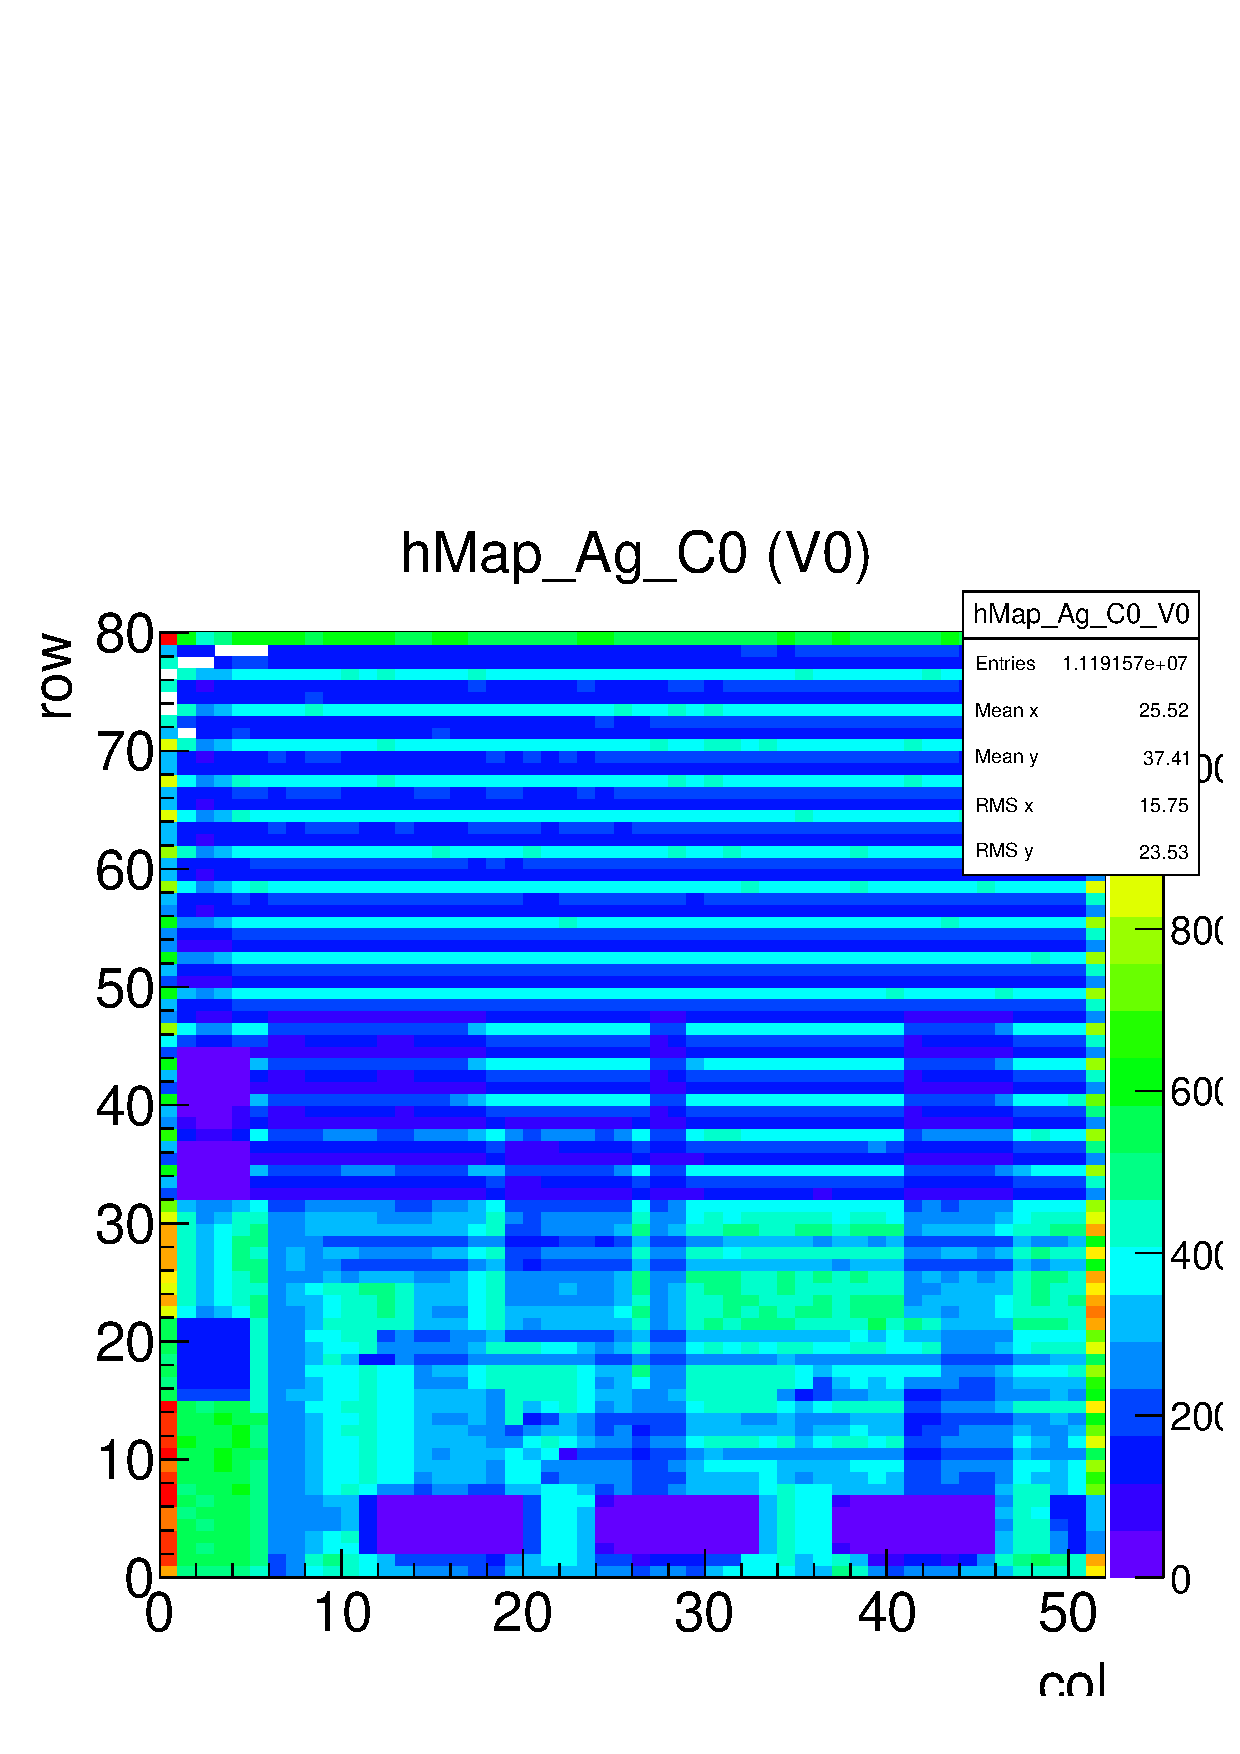
\includegraphics[width=\textwidth]{./HRData_Hitmap.pdf}
  \captionof{figure}{ROC map of the number of hits acquired per pixel.}
  \label{HRData-Hitmap}
\end{minipage}%
\hspace{2mm}
\begin{minipage}{.48\textwidth}
  \centering
  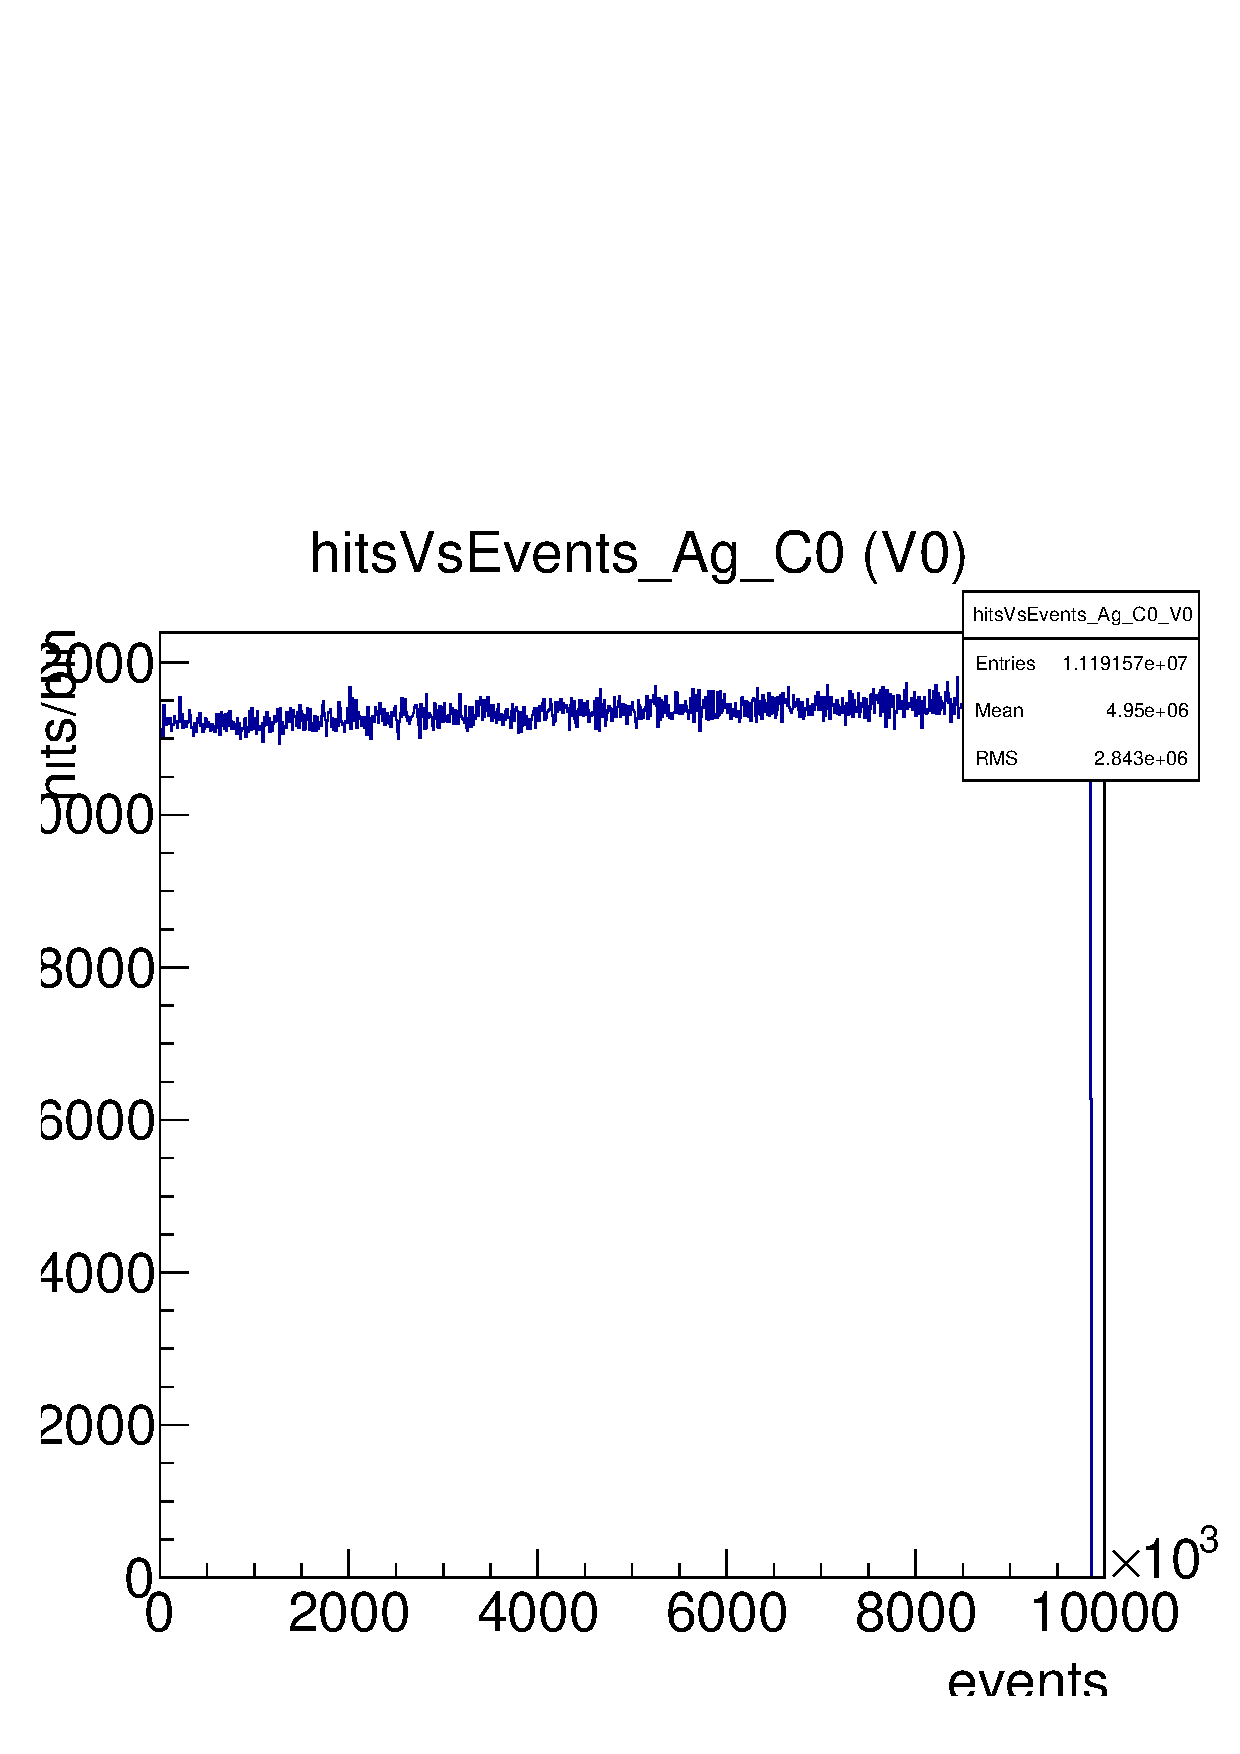
\includegraphics[width=\textwidth]{./HRData_HitsEvents.pdf}
  \captionof{figure}{Histogram showing the number of X-ray hits per event.}
  \label{HRData-HitsEvent}
\end{minipage}
\end{figure}

\begin{figure} [h!]
\centering
\begin{minipage}{.48\textwidth}
  \centering
  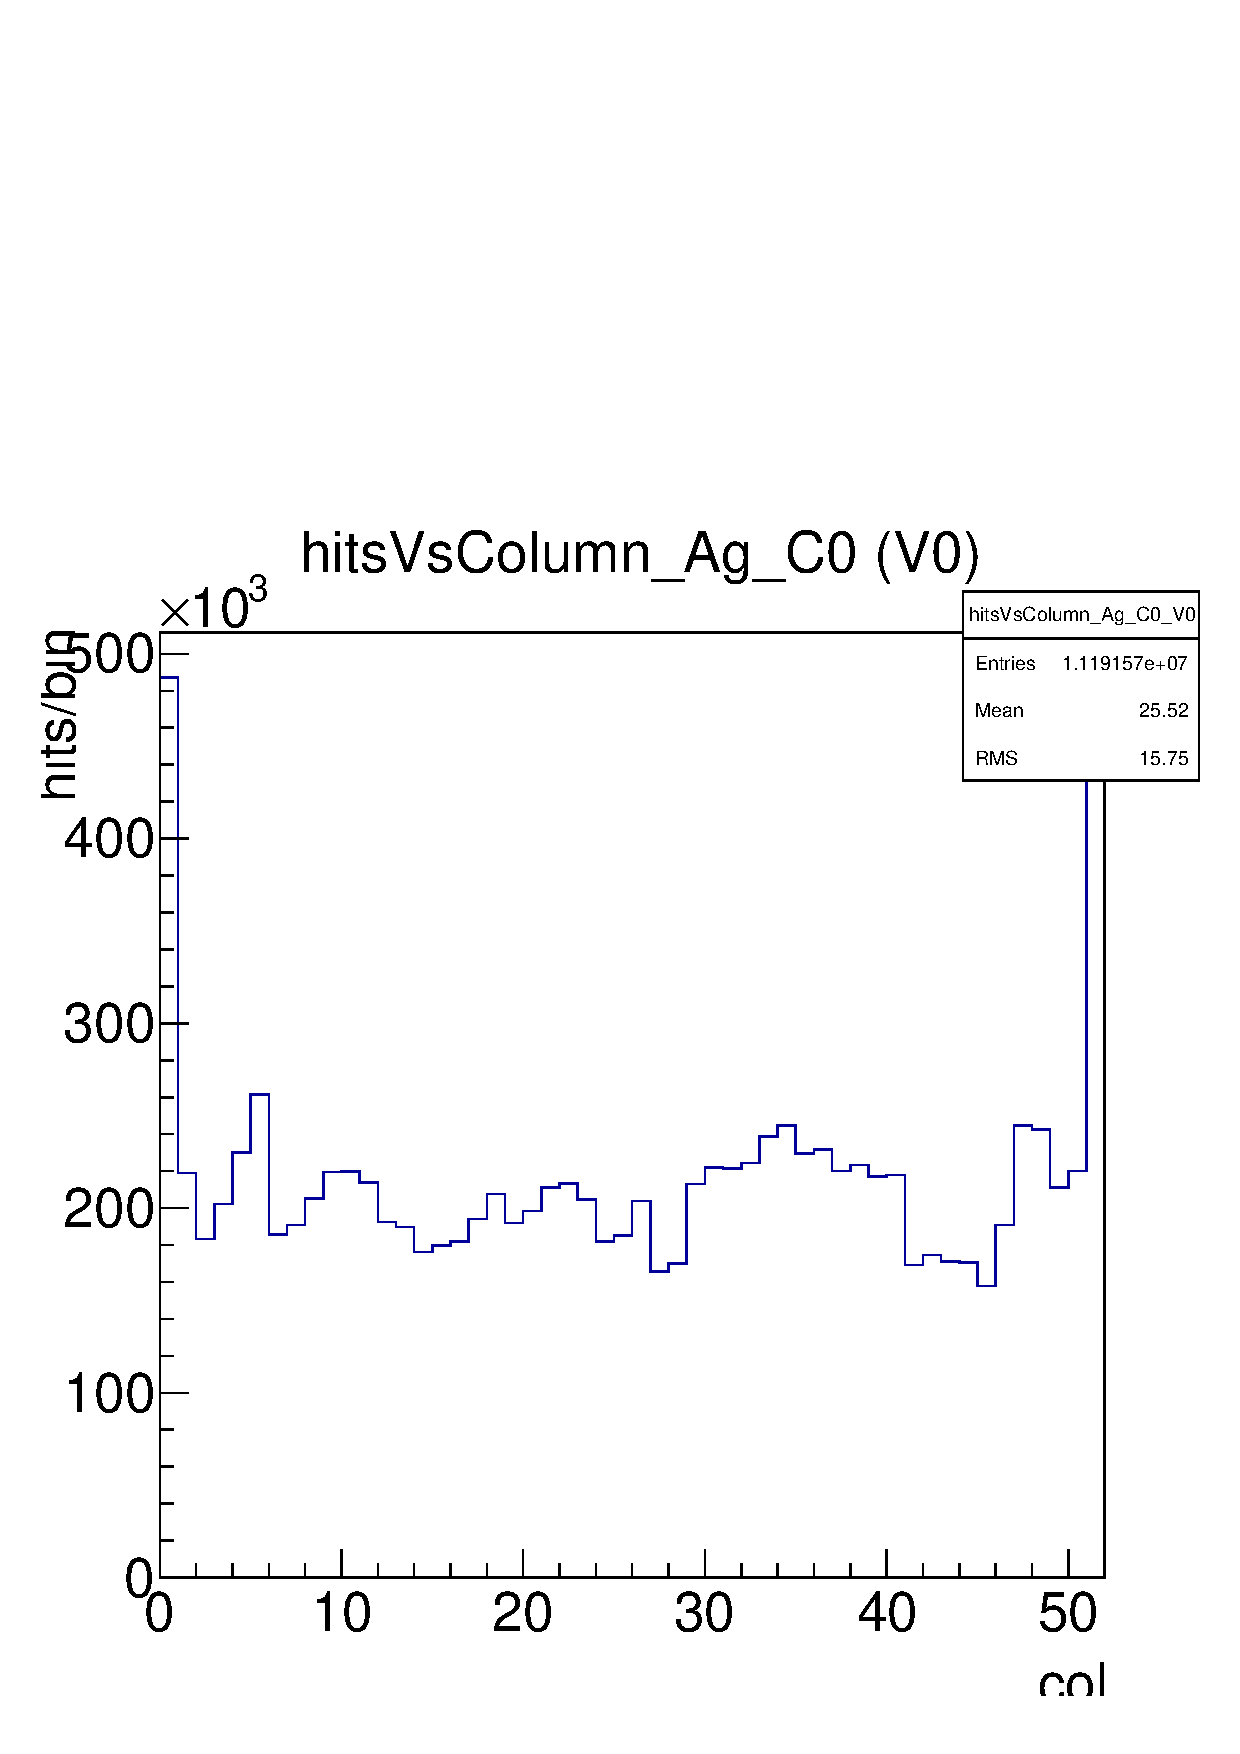
\includegraphics[width=\textwidth]{./HRData_HitsColumn.pdf}
  \captionof{figure}{Histogram showing the number of X-ray hits per column.}
  \label{HRData-HitsColumn}
\end{minipage}%
\hspace{2mm}
\begin{minipage}{.48\textwidth}
  \centering
  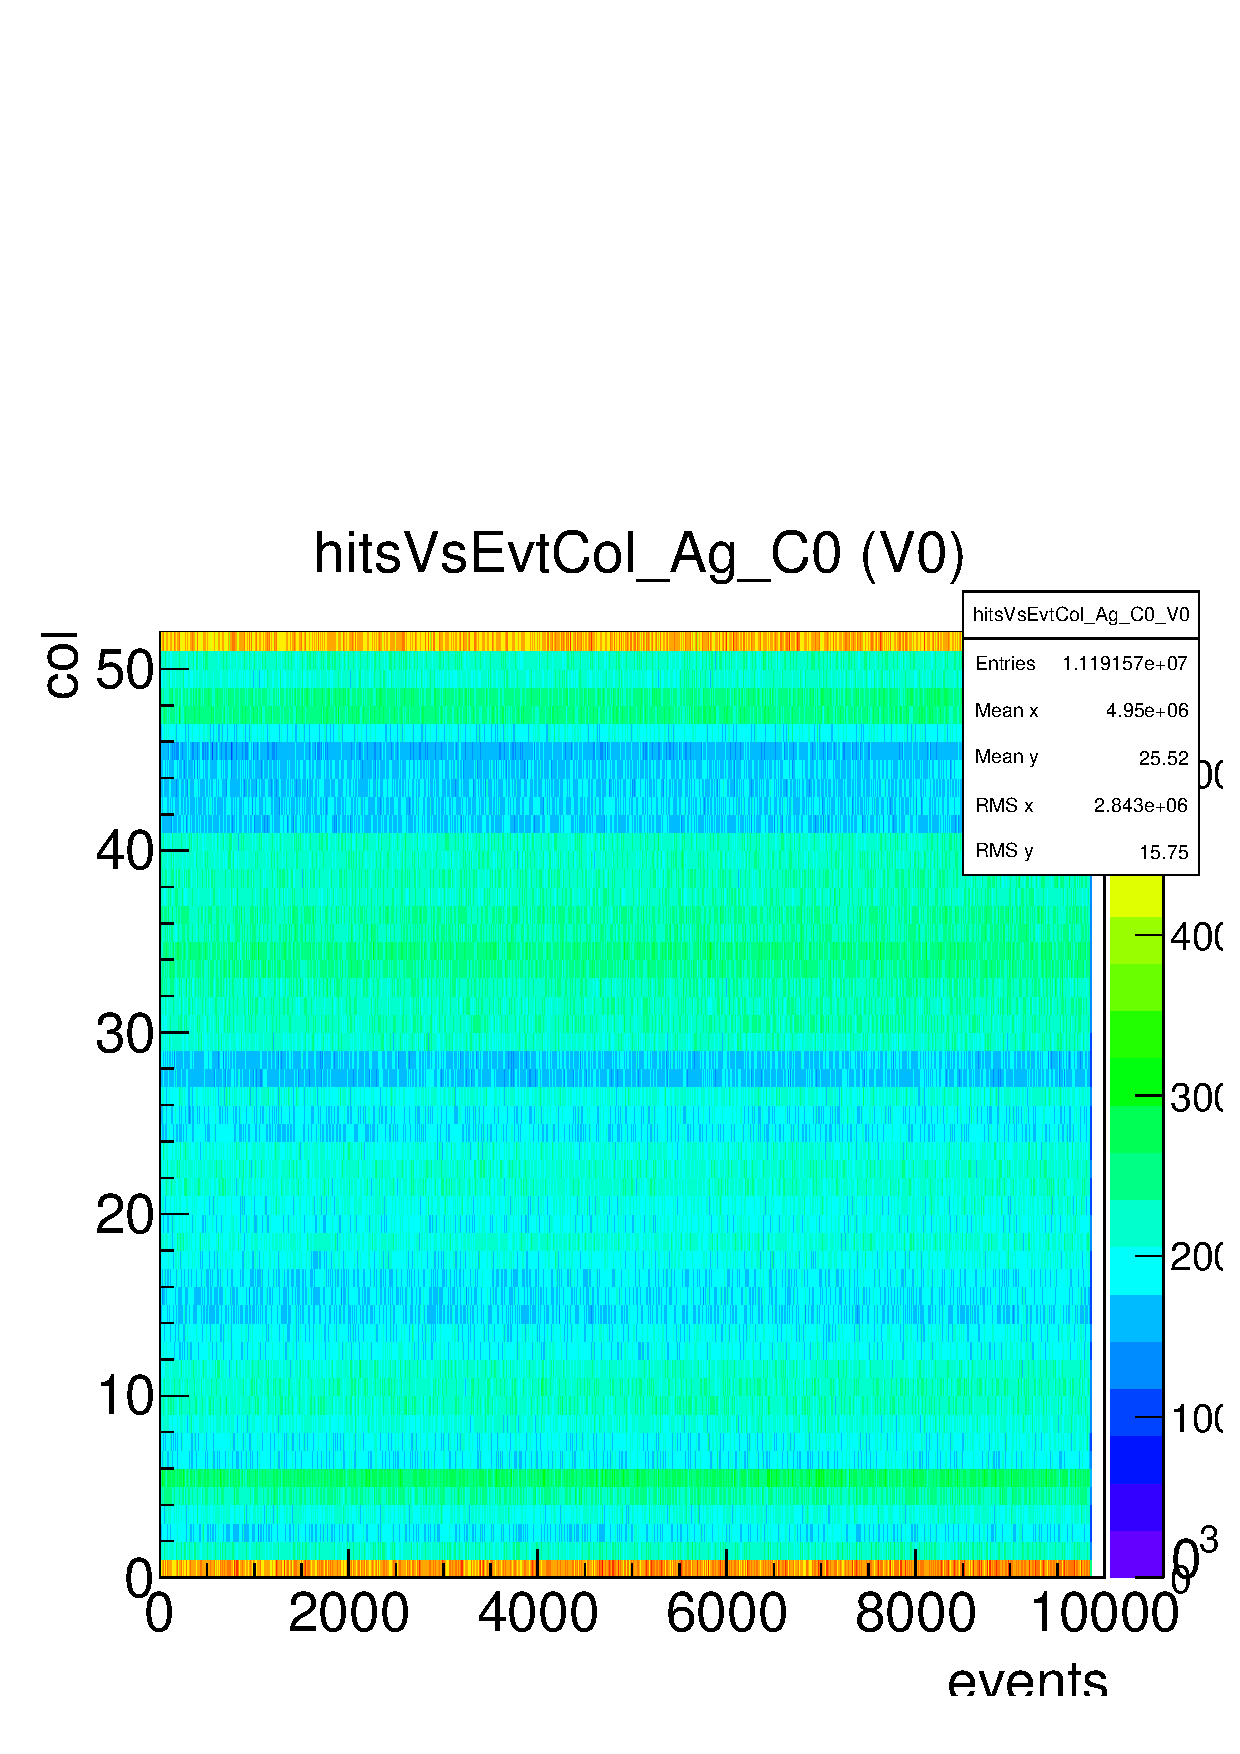
\includegraphics[width=\textwidth]{./HRData_HitsEventColumn.pdf}
  \captionof{figure}{Map showing the number of X-ray hits per event for every column.}
  \label{HRData-HitsEventColumn}
\end{minipage}
\end{figure}


\subsection{Xnoisemaps}
\subsubsection{Purpose}
This test aims to measure the electrical noise of each pixel. A similar test is performed in the FQ, but here all pixels are enabled and the module is exposed to X-radiation during the test which is not the case in the FQ.
\subsubsection{Methodology}
This test measured an SCurve for every pixel. To obtain it, a fixed number of test pulses are sent to every pixel and the number of correctly read-out pulses is recorded. This is done for many Vcal values around the threshold. The result is fitted with an error function, and the width around the half maximum is interpreted as the noise of the pixel.
\subsubsection{Output}
While the noise was already measured during the Full Qualification, it is remeasured here since it increases when all pixels are enabled (which is not the case in the FQ) and when the module is exposed to radiation. The noise measurement is performed in a similar way.

\begin{figure} [h!]
\centering
\begin{minipage}{.48\textwidth}
  \centering
  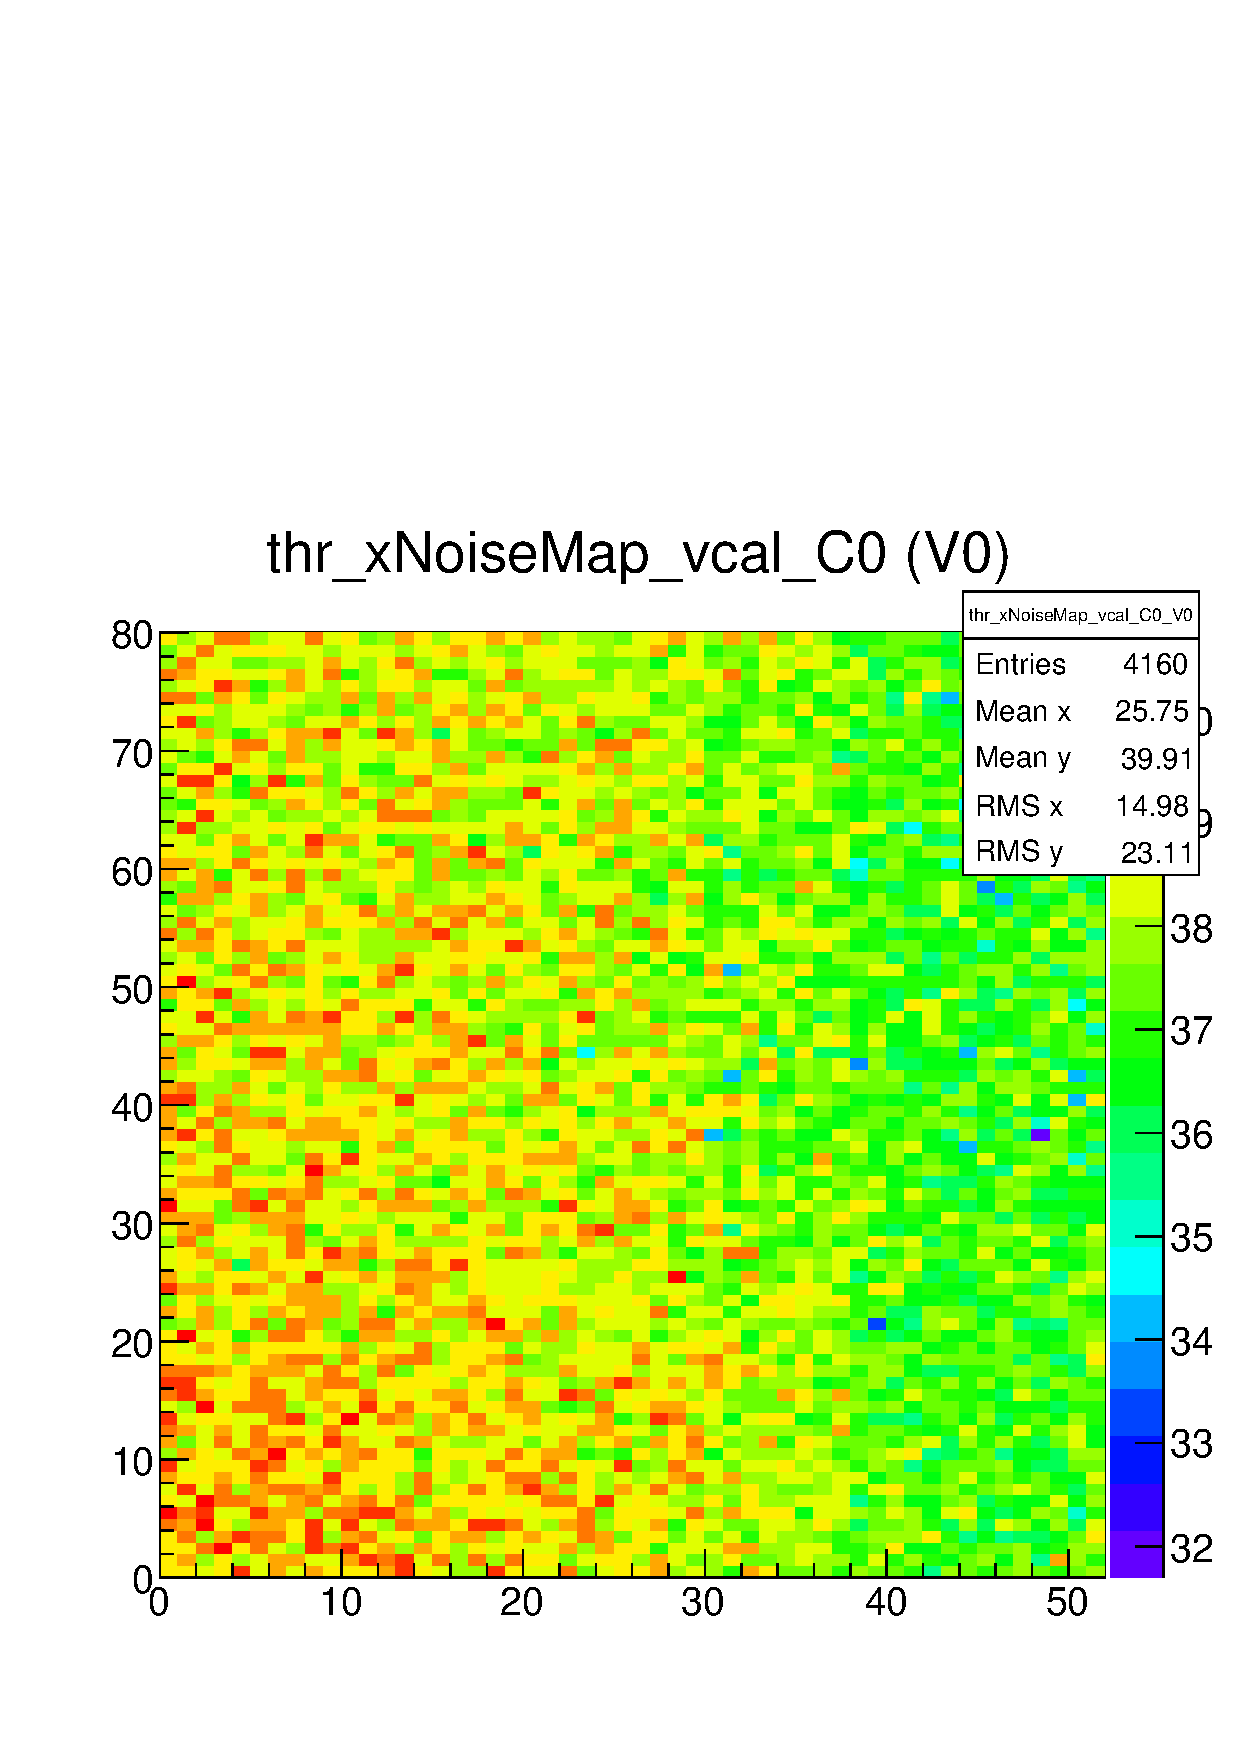
\includegraphics[width=\textwidth]{./HRSCurves_thrMap.pdf}
  \captionof{figure}{Map showing the measured threshold for every pixel.}
  \label{HRSCurves-thrMap}
\end{minipage}%
\hspace{2mm}
\begin{minipage}{.48\textwidth}
  \centering
  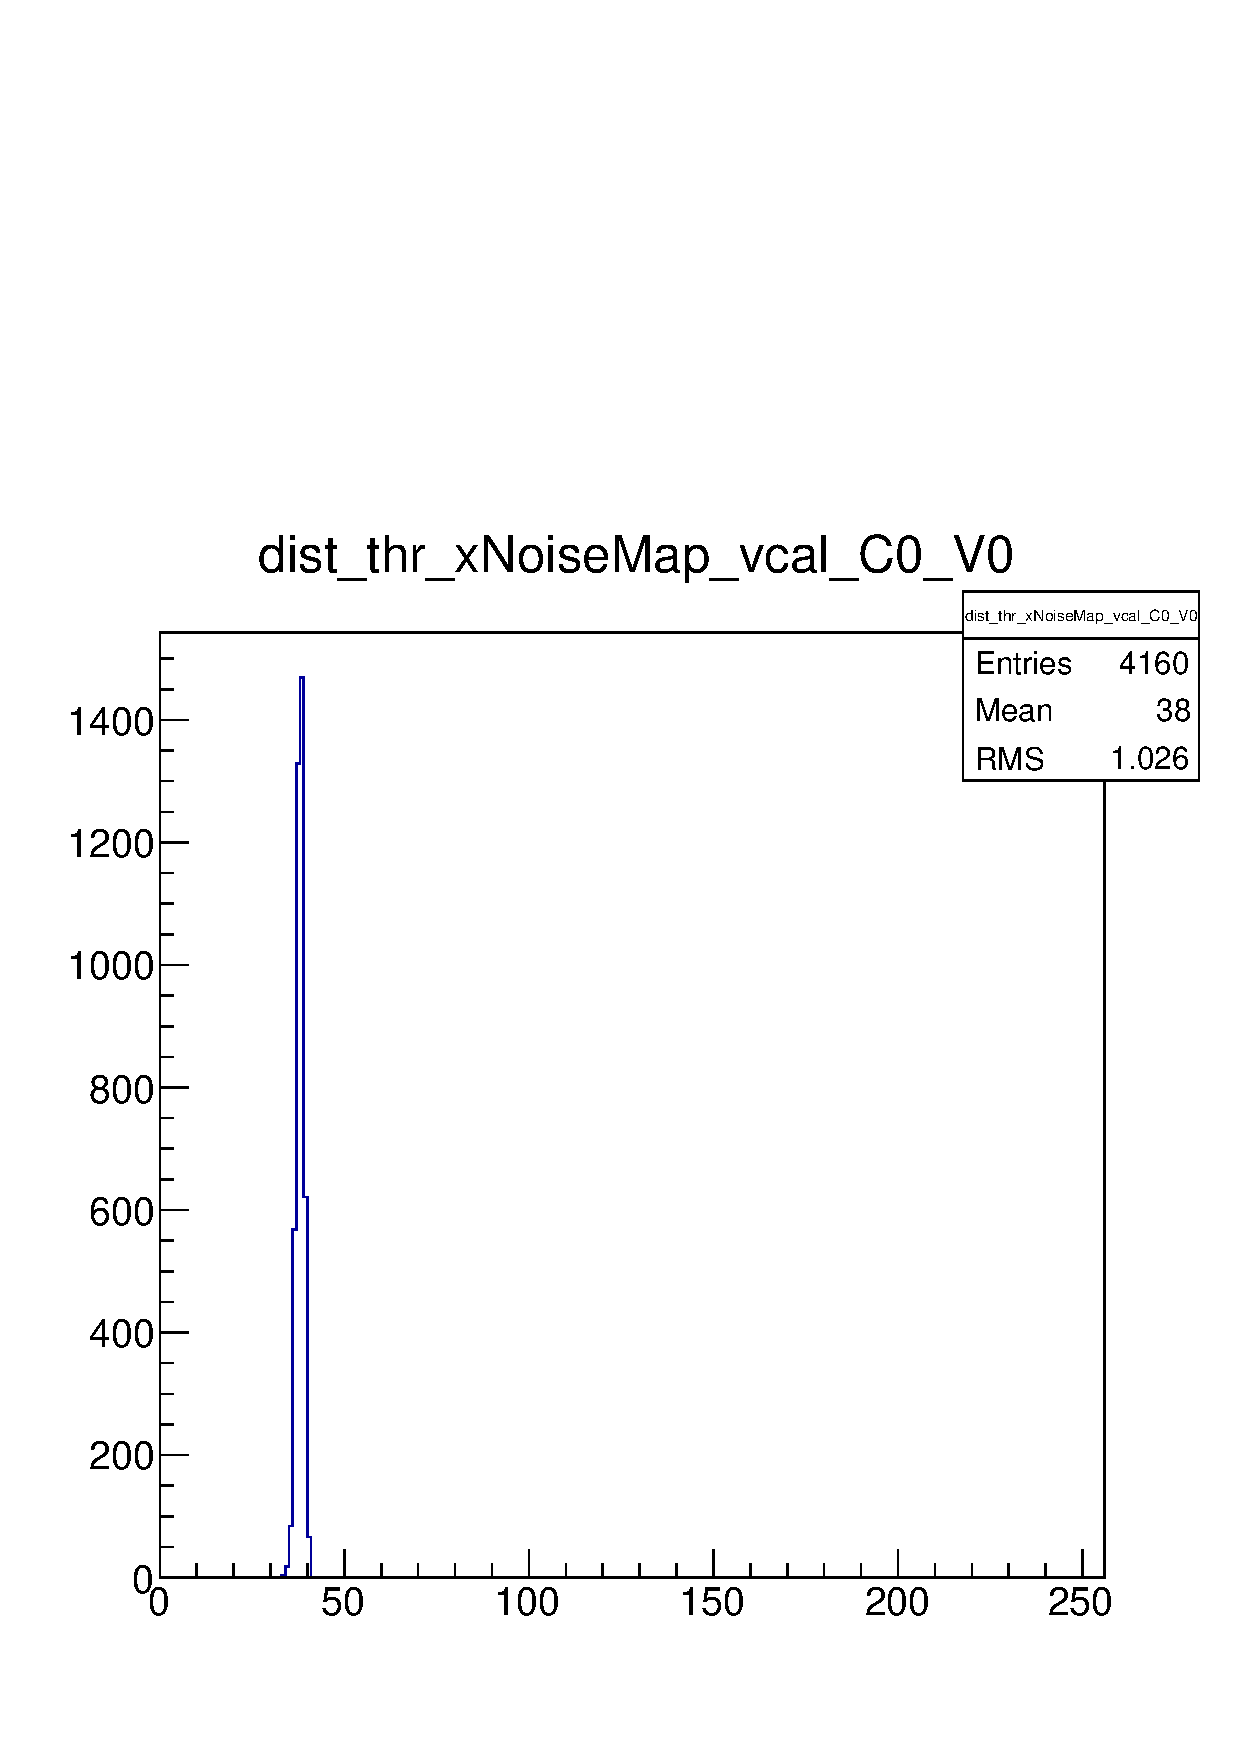
\includegraphics[width=\textwidth]{./HRSCurves_thrDist.pdf}
  \captionof{figure}{Histogram of the threshold of every pixel.}
  \label{HRSCurves-thrDist}
\end{minipage}
\end{figure}

\begin{figure} [h!]
\centering
\begin{minipage}{.48\textwidth}
  \centering
  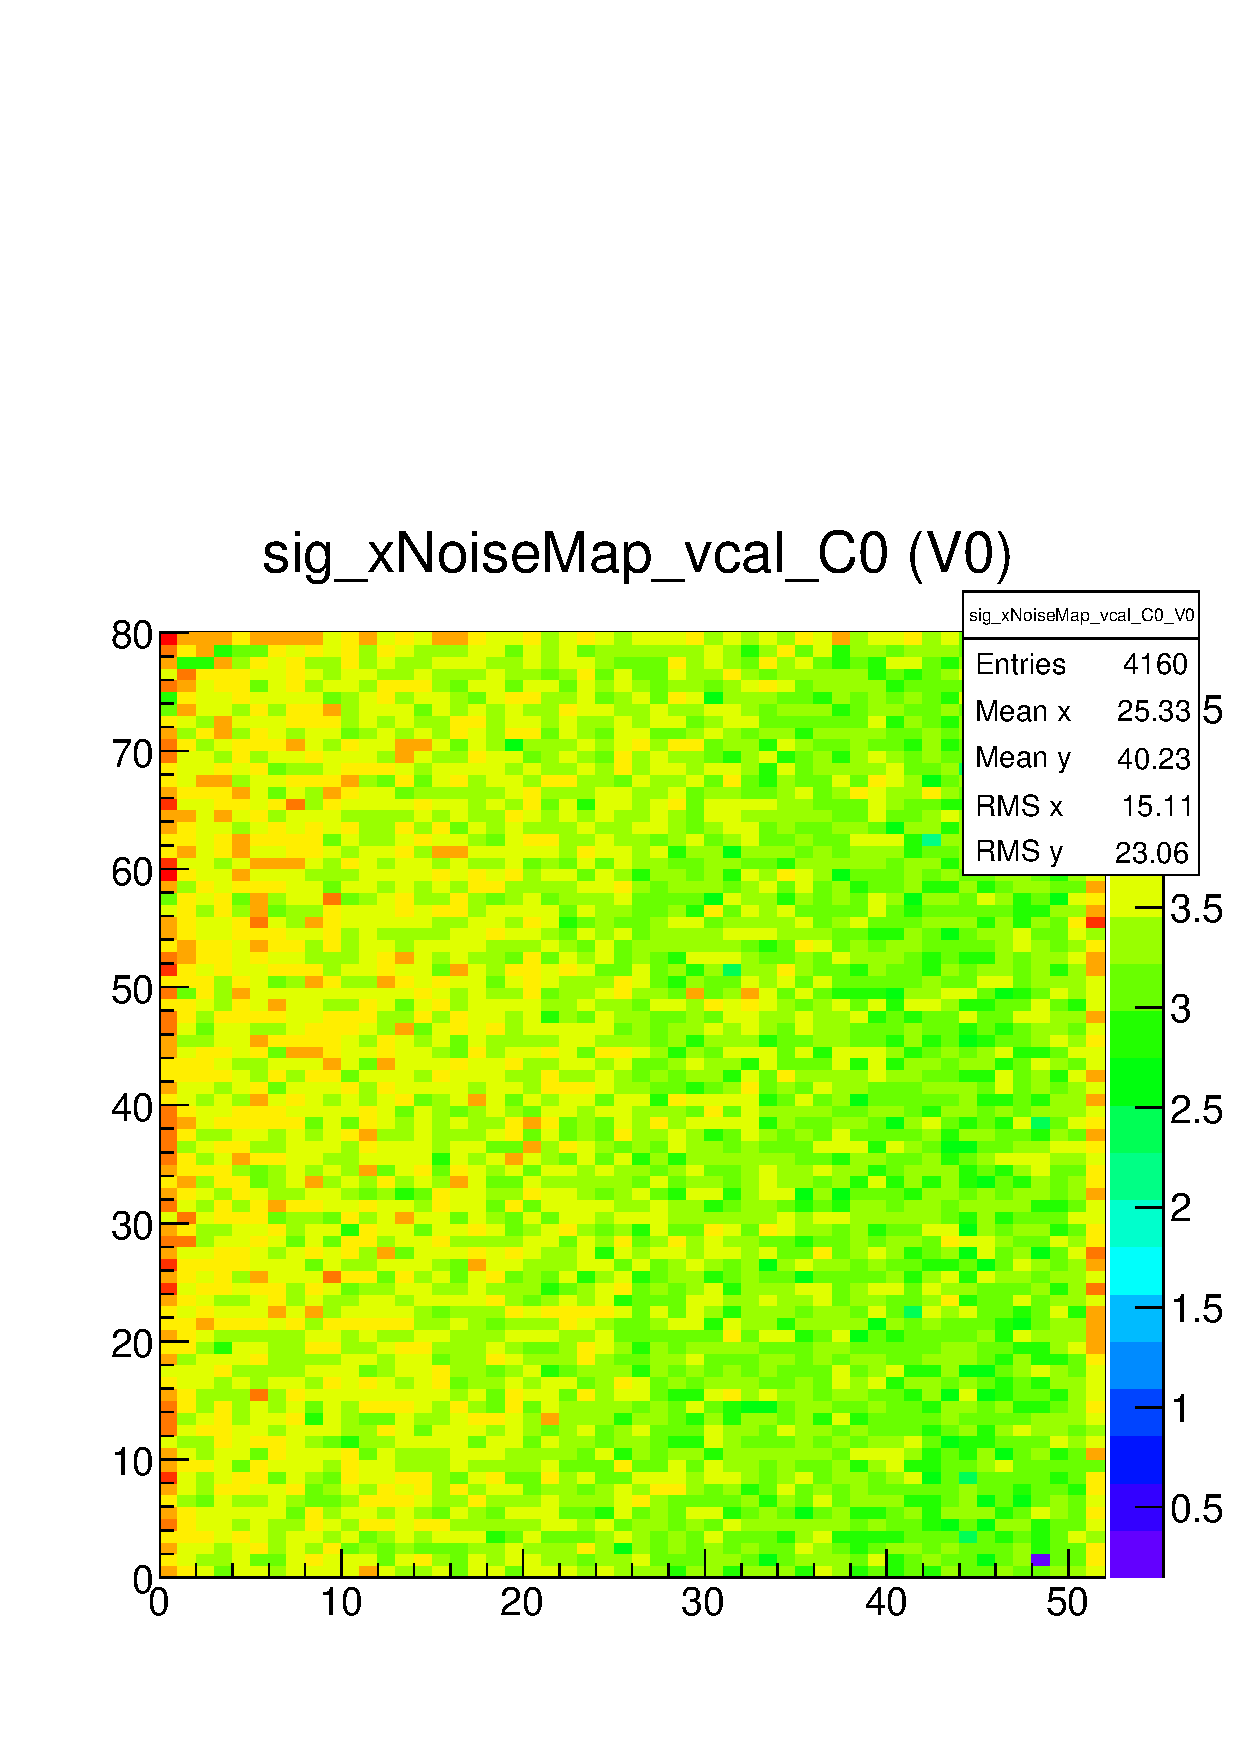
\includegraphics[width=\textwidth]{./HRSCurves_sigMap.pdf}
  \captionof{figure}{Map showing the measured noise for every pixel.}
  \label{HRSCurves-sigMap}
\end{minipage}%
\hspace{2mm}
\begin{minipage}{.48\textwidth}
  \centering
  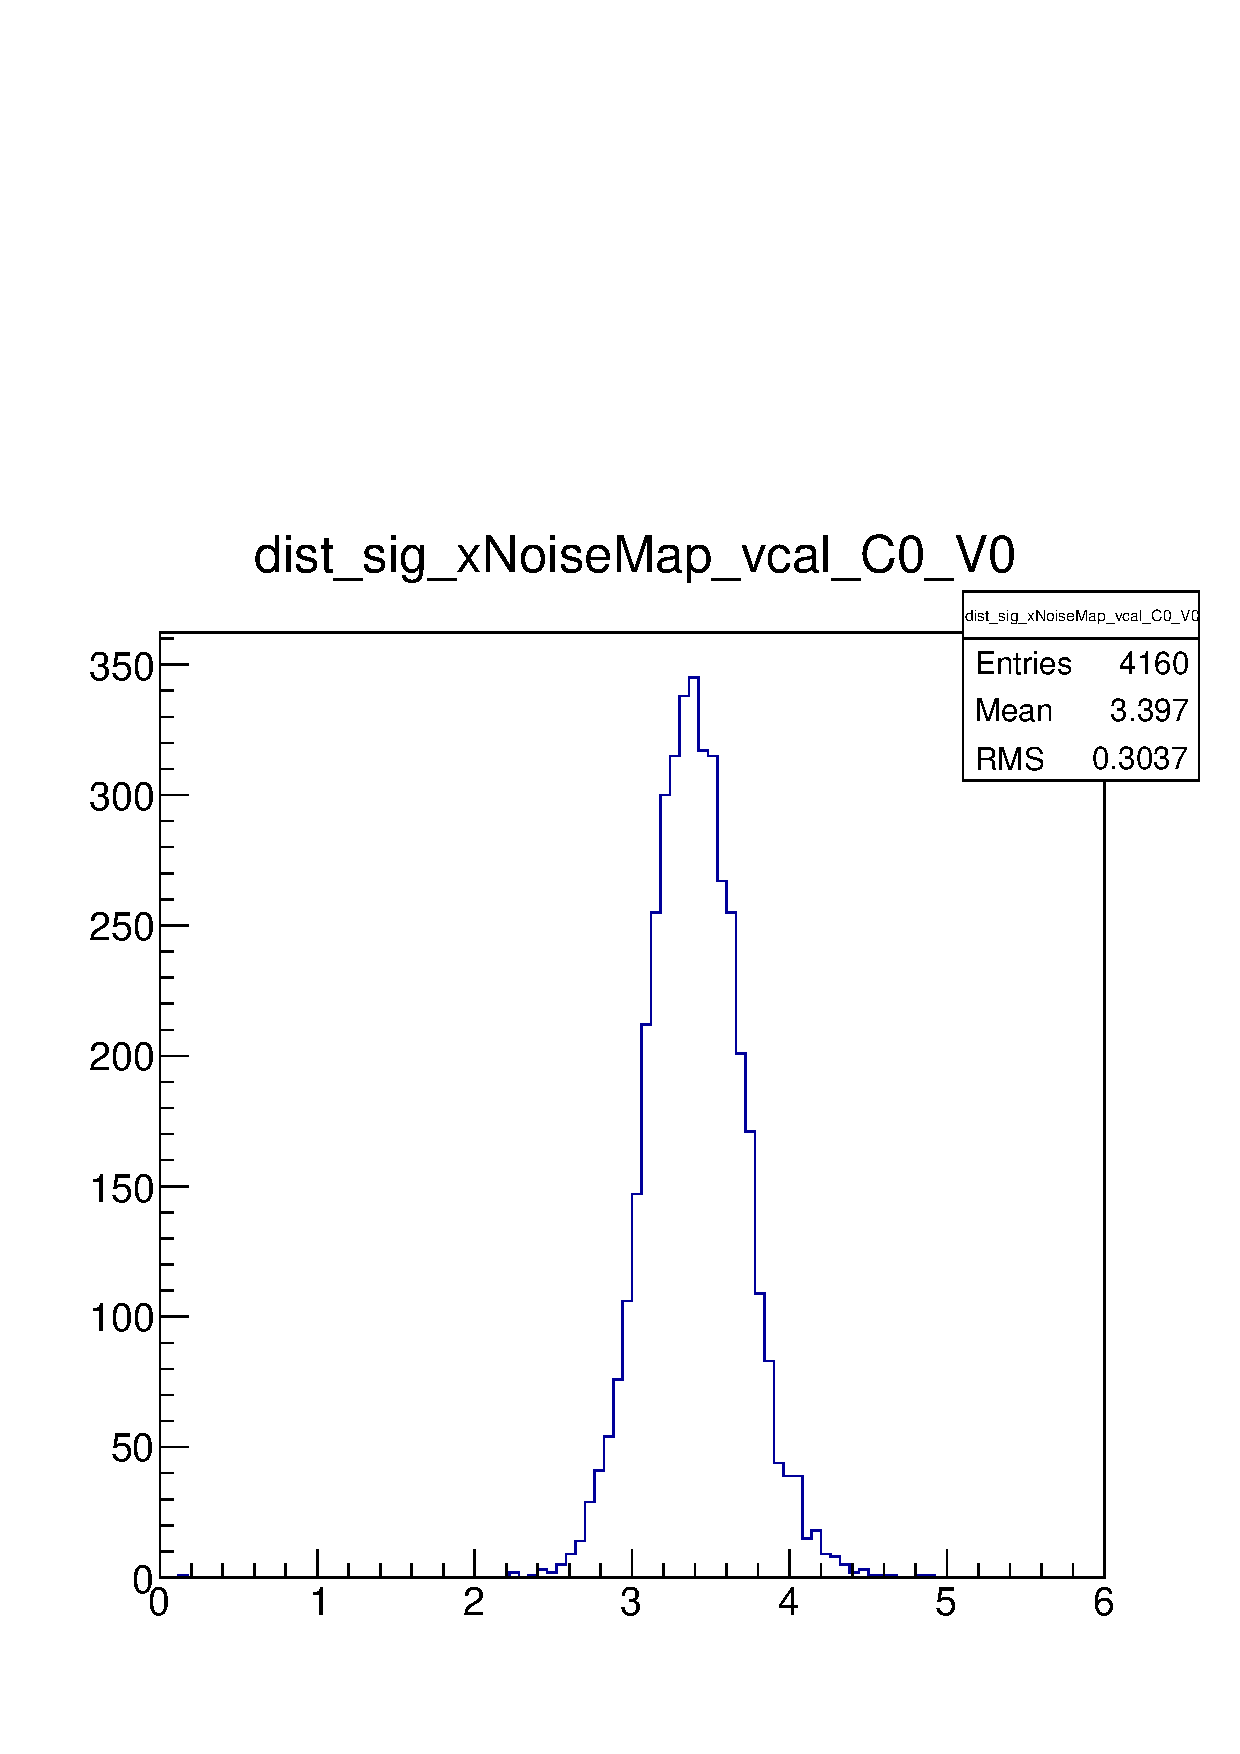
\includegraphics[width=\textwidth]{./HRSCurves_sigDist.pdf}
  \captionof{figure}{Histogram of the noise of every pixel.}
  \label{HRSCurves-sigDist}
\end{minipage}
\end{figure}

\begin{figure} [h!]
\centering
\begin{minipage}{.48\textwidth}
  \centering
  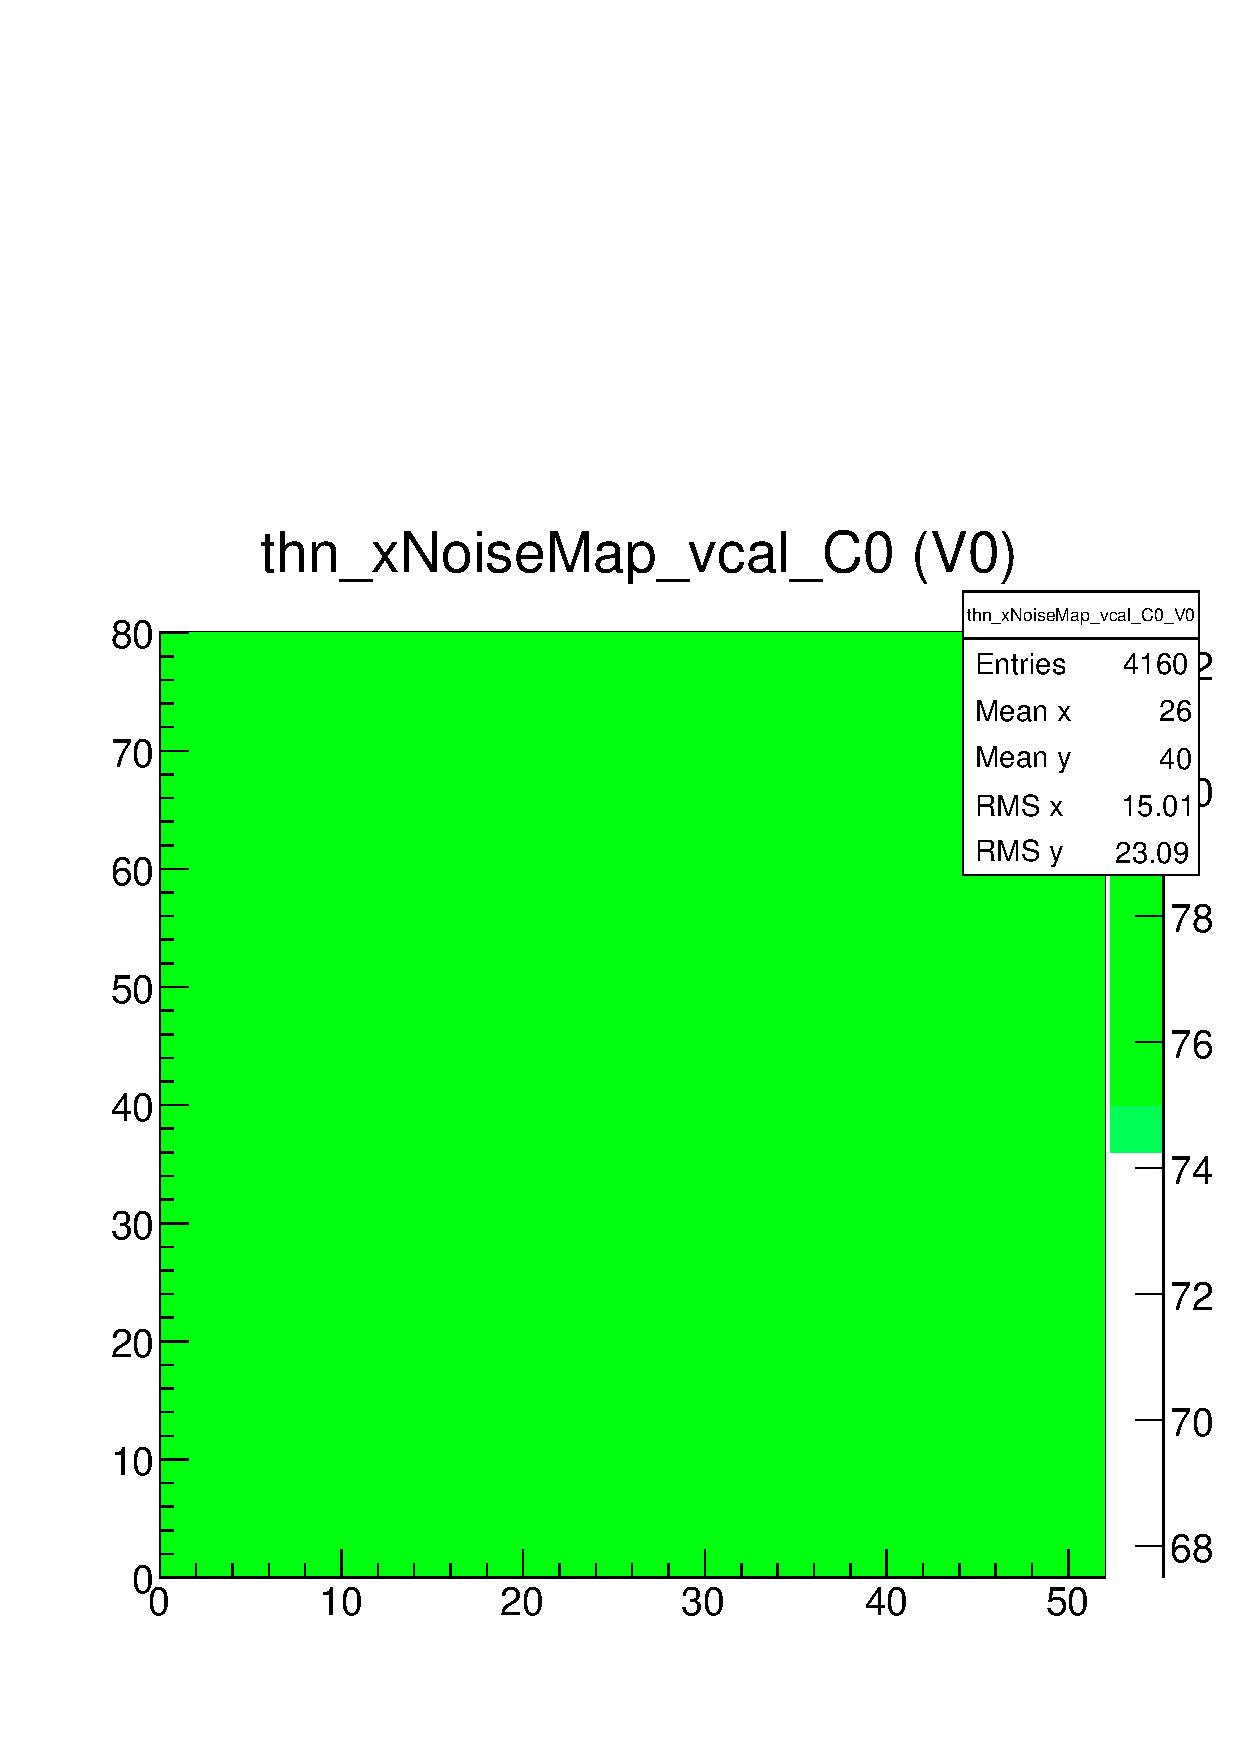
\includegraphics[width=\textwidth]{./HRSCurves_thnMap.pdf}
  \captionof{figure}{Map showing the measured turn-on threshold for every pixel.}
  \label{HRSCurves-thnMap}
\end{minipage}%
\hspace{2mm}
\begin{minipage}{.48\textwidth}
  \centering
  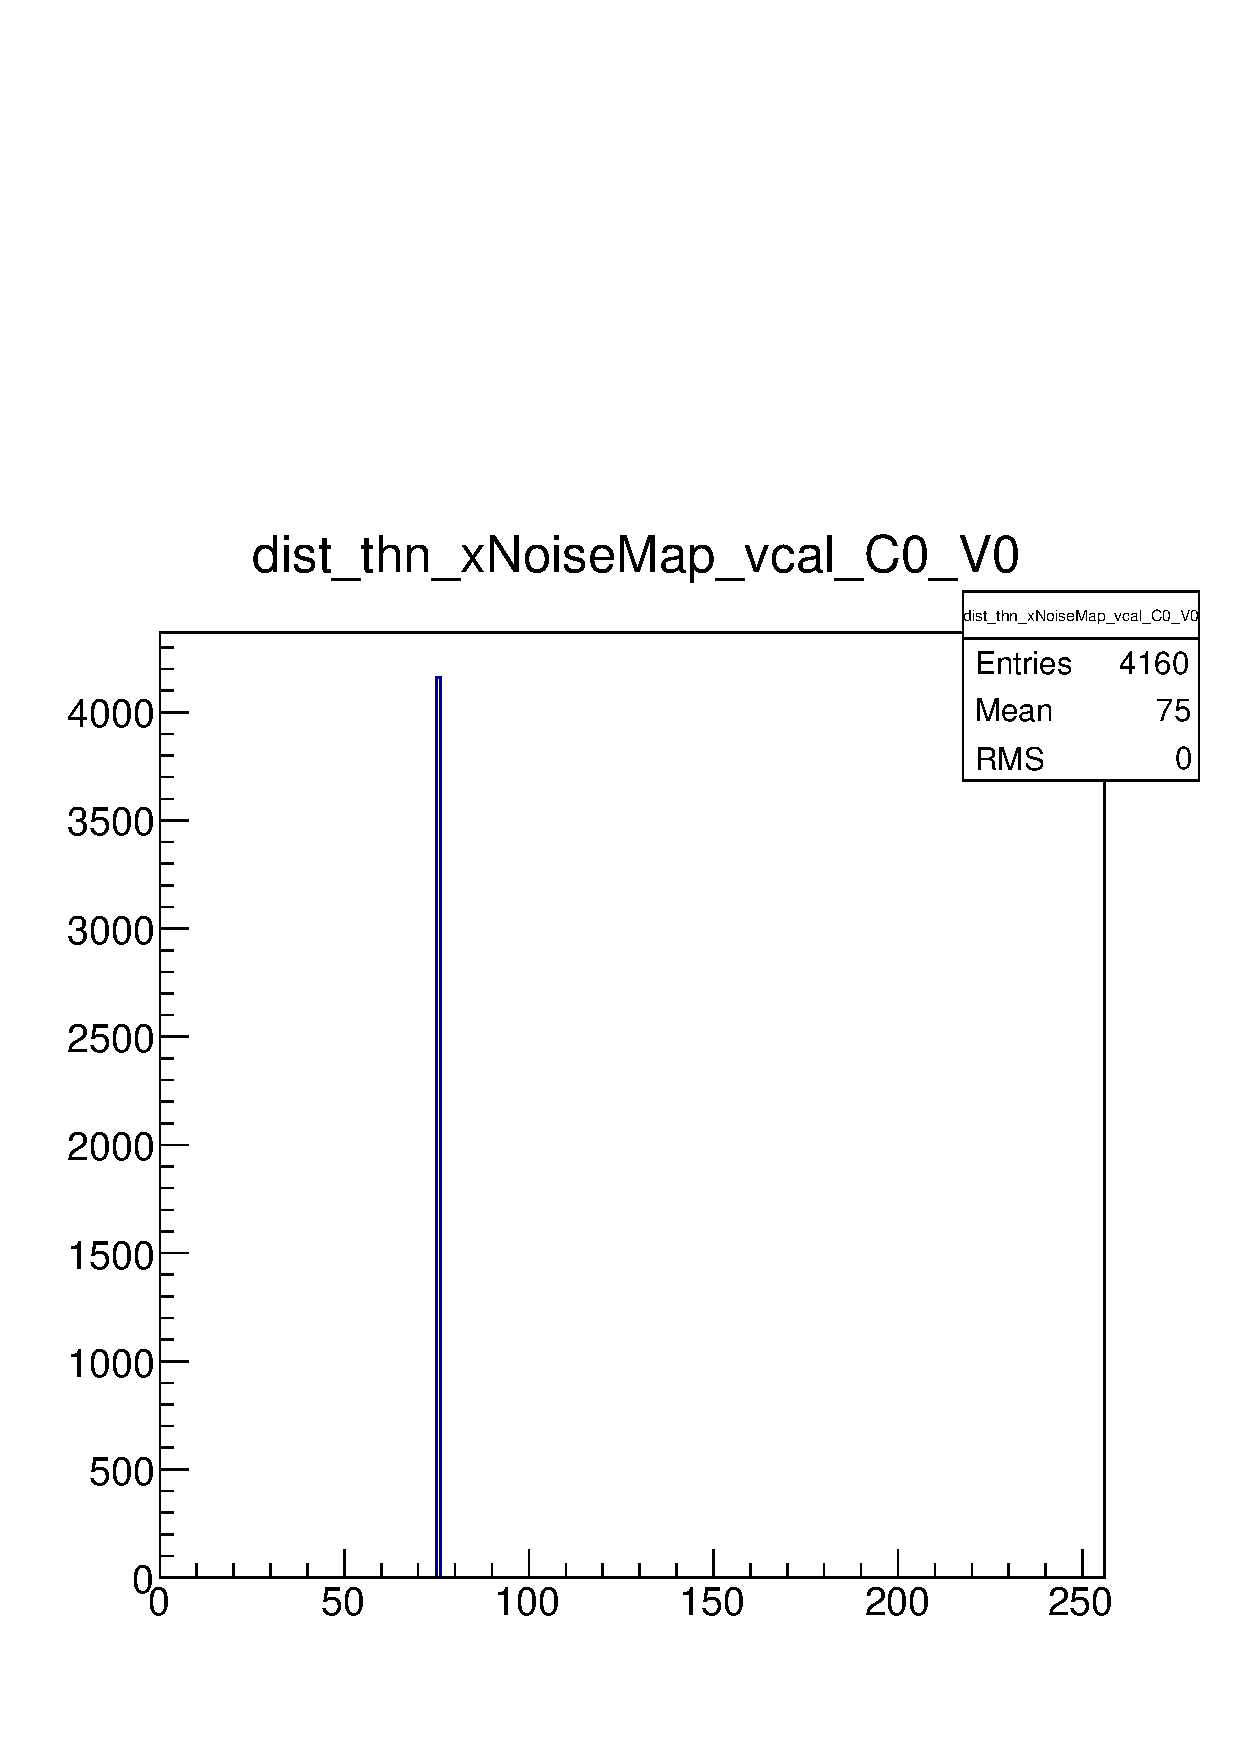
\includegraphics[width=\textwidth]{./HRSCurves_thnDist.pdf}
  \captionof{figure}{Histogram of the turn-on threshold of every pixel.}
  \label{HRSCurves-thnDist}
\end{minipage}
\end{figure}



\subsection{Caldelscan}

\subsubsection{Purpose}
The efficiency of a ROC is slightly varying with the CalDel DAC. It is therefore optimized before the efficiency measurement.

\subsubsection{Measurement}
The first step in the optimization of CalDel is to see for which of its values test pulses can be read out (see Figure~\ref{CalDel-Scan}). To this aim, a set number of pulses for every CalDel value are sent to a single pixel, and the number of detected pulses is then read out. The valid range of CalDel values is then all DAC values for which the number of detected test pulses is at least 80\% of the maximum. For safety and to cope with small variations amongst all pixels of a ROC, the lowest and highest CalDel values are excluded. Once the CalDel range has been found, the efficiency is measured for all pixels for a set of CalDel values within that range. Examples are found in Figures~\ref{CalDel-Step0} and \ref{CalDel-Step5} which show a histogram of the efficiency of all pixels for the first and the sixth CalDel that is tested. The efficiency is the fraction of correctly read-out test pulses. The mean efficiency of all pixels is evaluated for every pixel and plotted in a histogram (see Figure~\ref{CalDel-Efficiency}). The final chosen CalDel value is the value of that DAC where the efficiency is highest.

\subsubsection{Output}
\begin{figure} [h!]
\centering
\begin{minipage}{.48\textwidth}
  \centering
  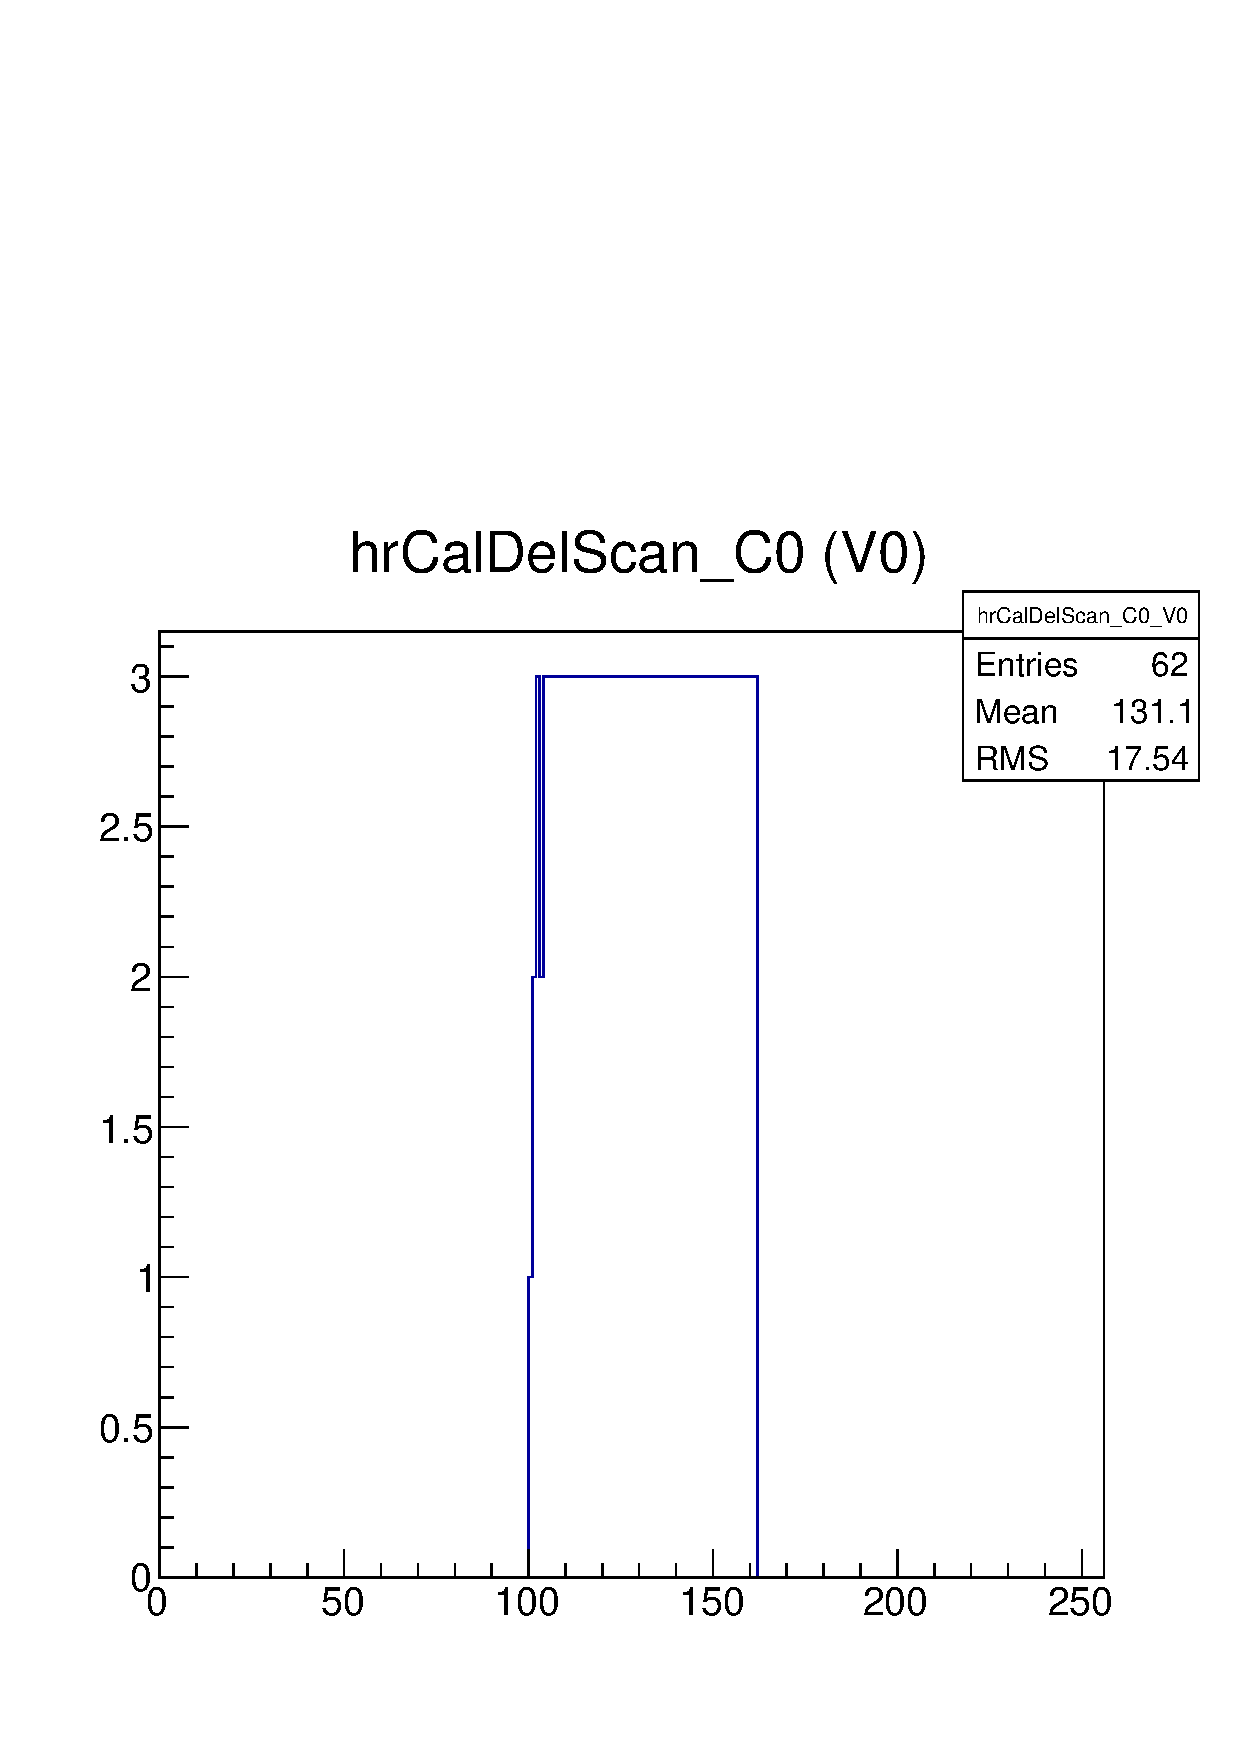
\includegraphics[width=\textwidth]{./CalDel_CalDelScan.pdf}
  \captionof{figure}{CalDel scan of ROC 0.}
  \label{CalDel-Scan}
\end{minipage}%
\hspace{2mm}
\begin{minipage}{.48\textwidth}
  \centering
  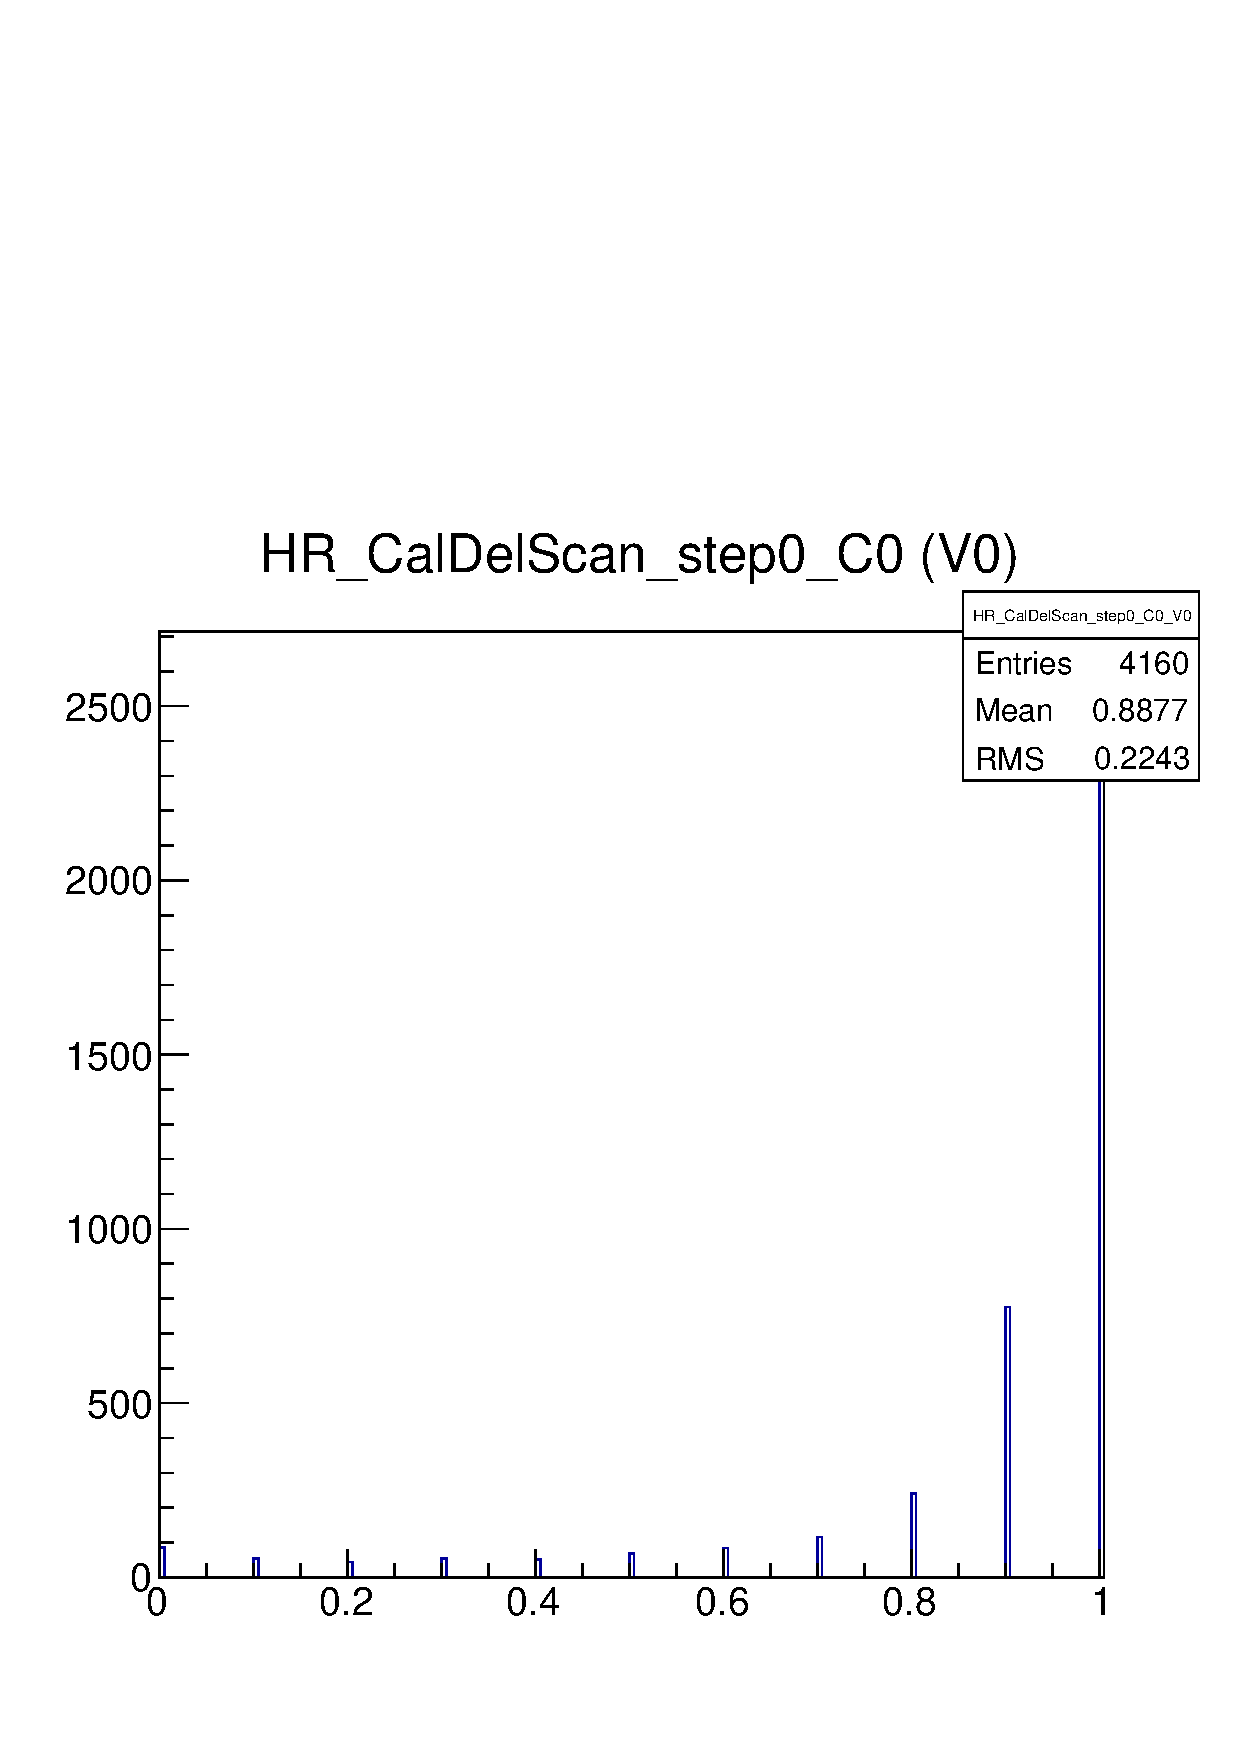
\includegraphics[width=\textwidth]{./CalDel_Step0.pdf}
  \captionof{figure}{Efficiency of ROC 0 with first tested CalDel}
  \label{CalDel-Step0}
\end{minipage}
\end{figure}

\begin{figure} [h!]
\centering
\begin{minipage}{.48\textwidth}
  \centering
  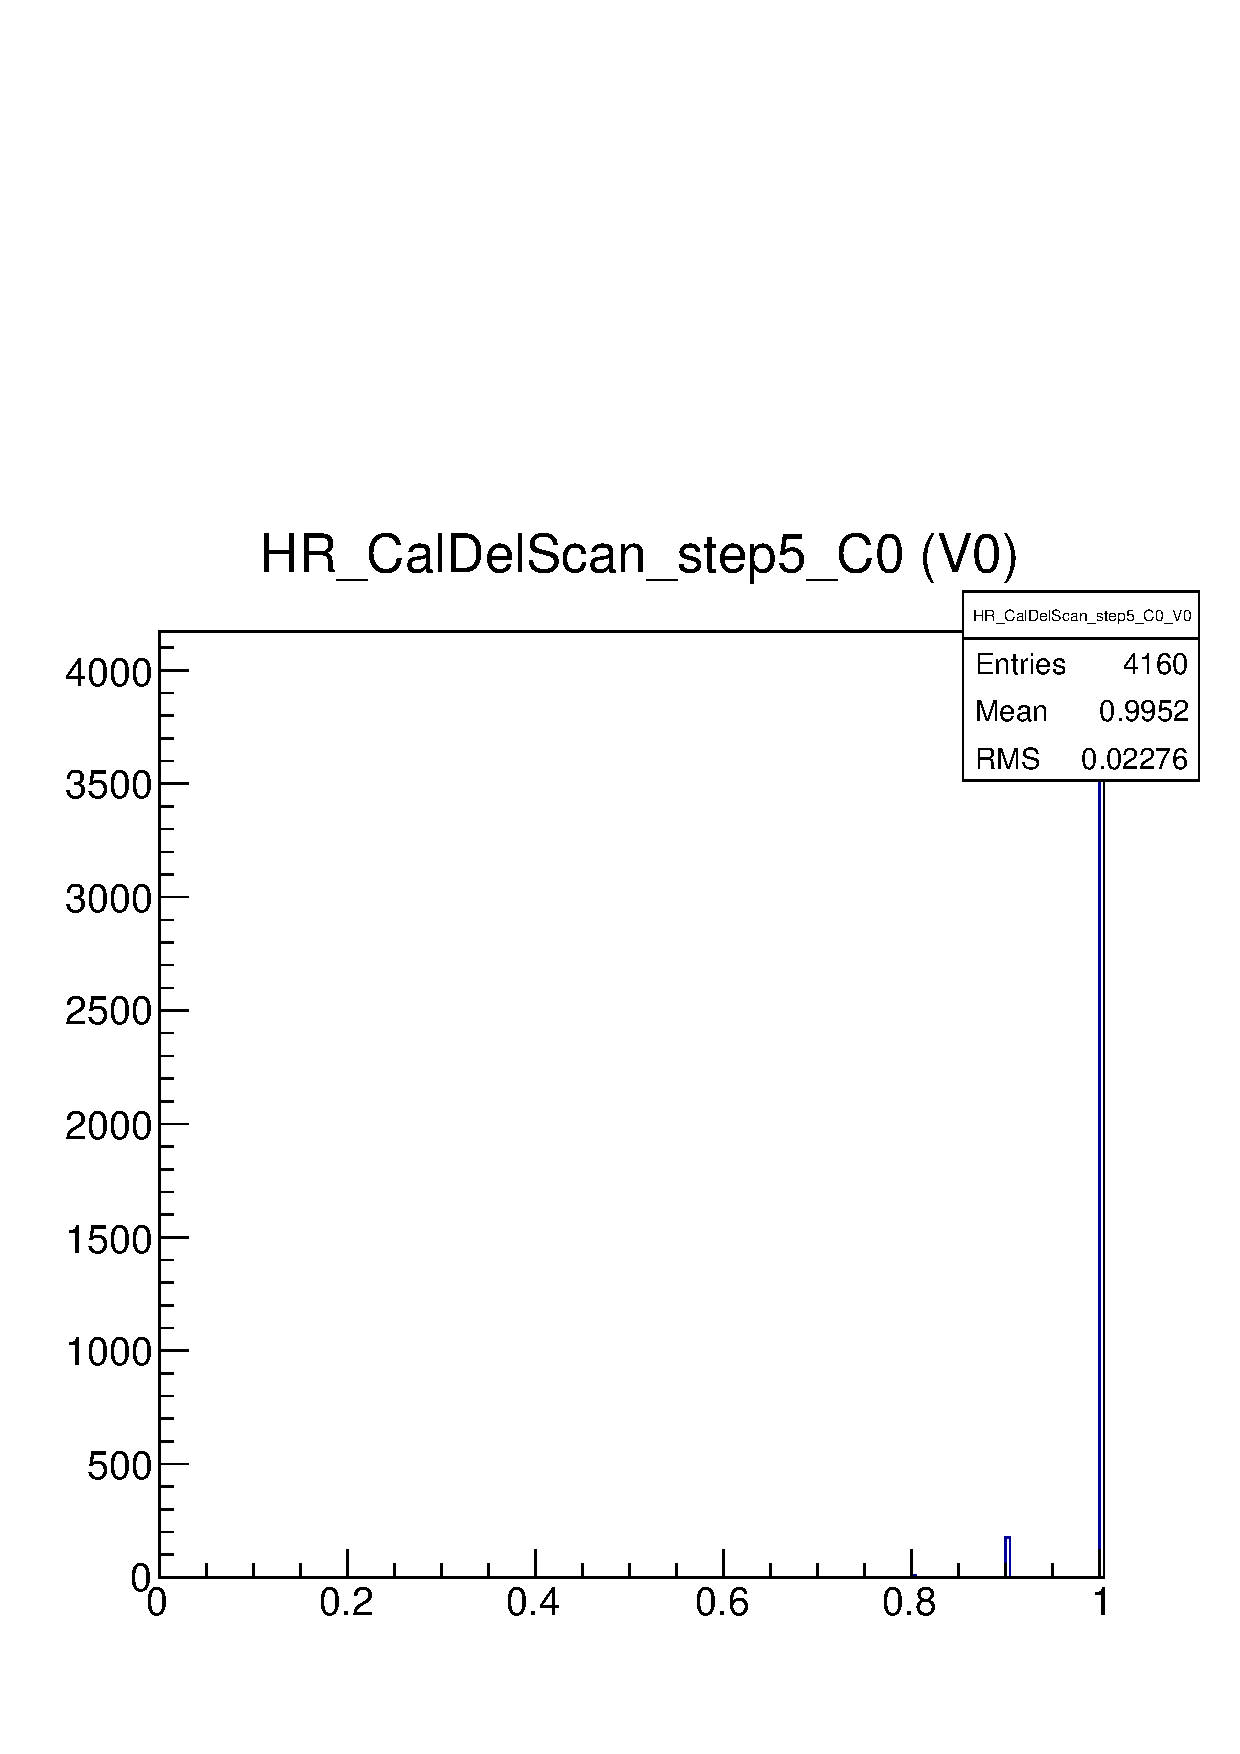
\includegraphics[width=\textwidth]{./CalDel_Step5.pdf}
  \captionof{figure}{Efficiency of ROC 0 with sixth tested CalDel.}
  \label{CalDel-Step5}
\end{minipage}%
\hspace{2mm}
\begin{minipage}{.48\textwidth}
  \centering
  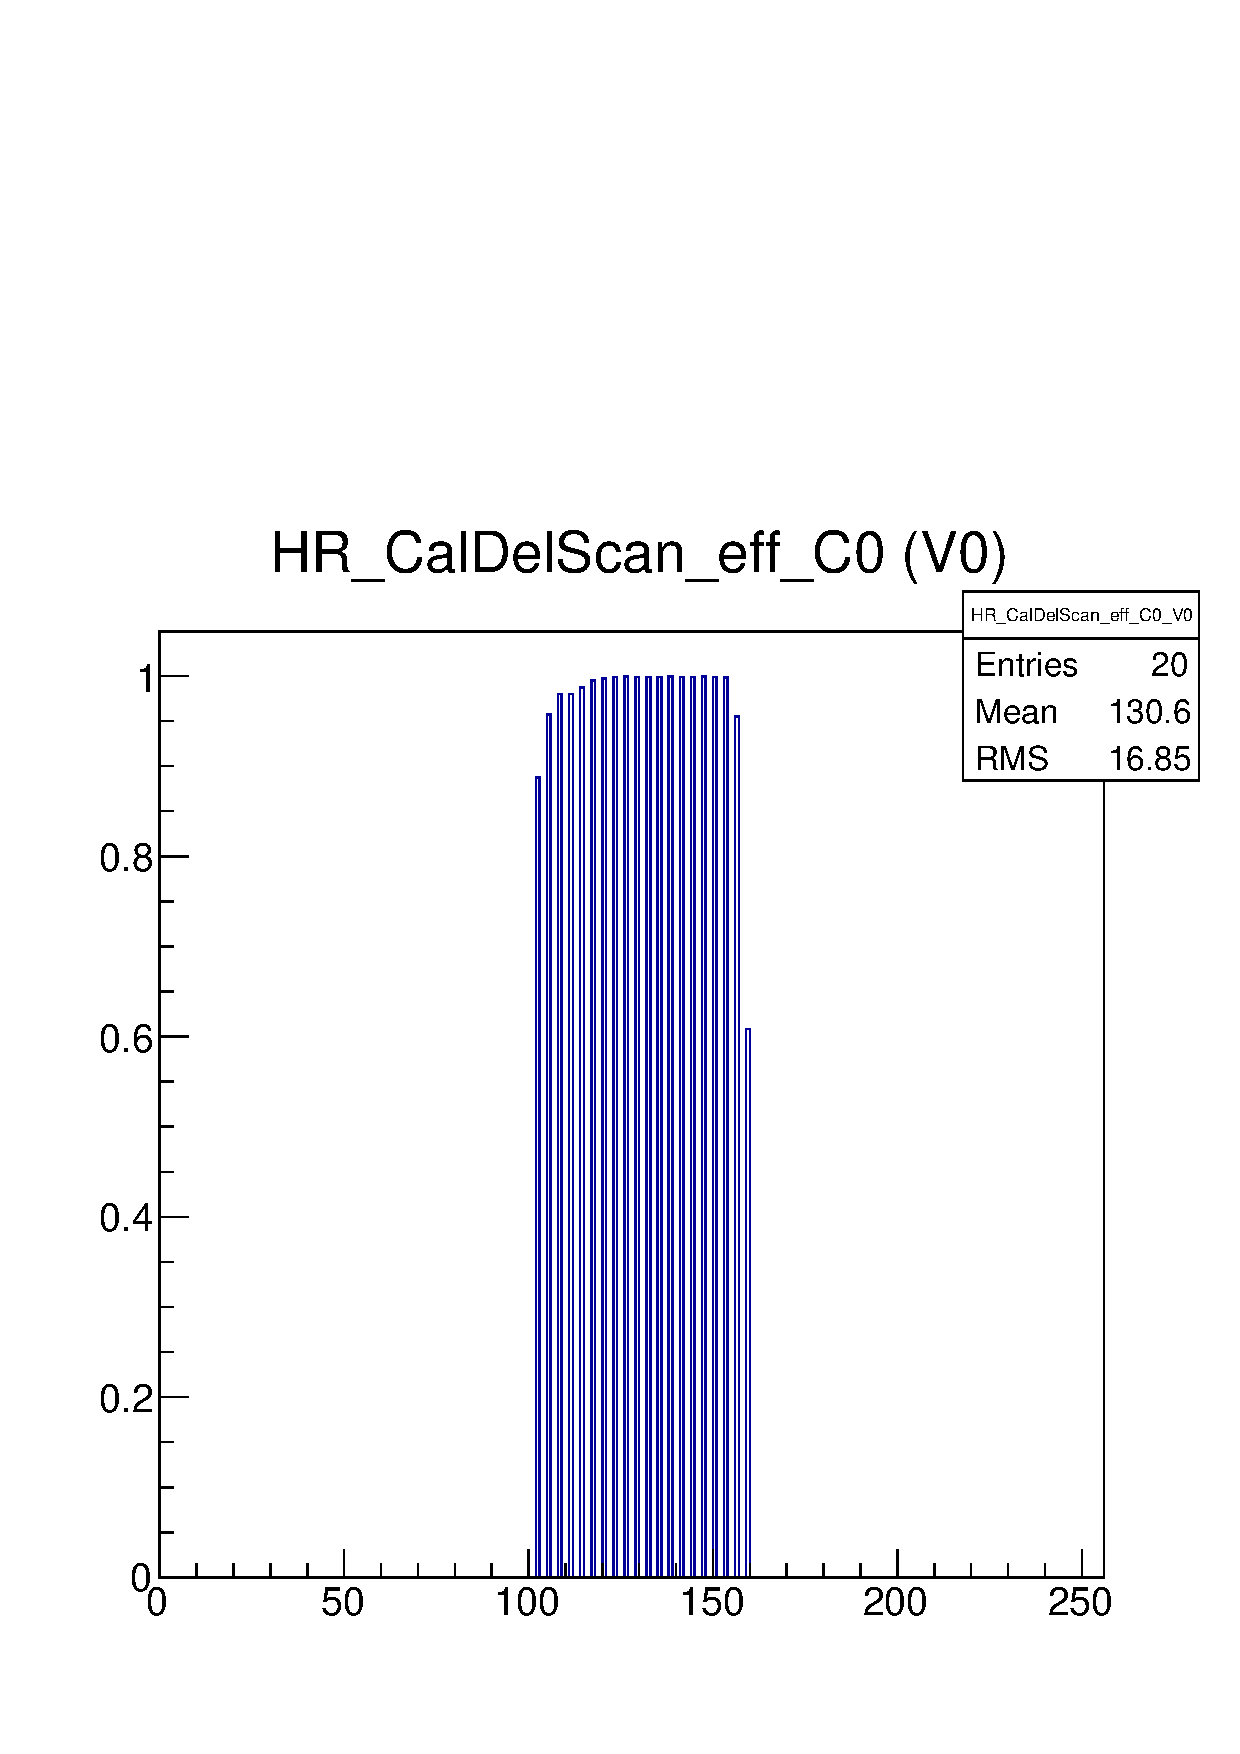
\includegraphics[width=\textwidth]{./CalDel_Efficiency.pdf}
  \captionof{figure}{Efficiency of each pixel on the ROC as a function of CalDel.}
  \label{CalDel-Efficiency}
\end{minipage}
\end{figure}

\subsection{Xpixelalive}

\subsubsection{Purpose}

This test aims to measure the efficiency of each pixel at a measured pixel hit rate.

\subsubsection{Measurement}

This test is performed while exposing the module to X-radiation. A fixed number of test pulses are sent to every pixel, and the number of correctly read-out pulses is recorded (see Figure~\ref{Efficiency-Map}). The efficiency is the fraction of test pulses which is read out correctly and is plotted for every pixel in Figure~\ref{Efficiency-Overall}. Due to their larger size and to their usually higher noise, the efficiency of edge pixels is lower for fro a fixed X-ray rate. This is why the fiducial efficiency is also evaluated (see Figure~\ref{Efficiency-Fiducial}). Here
the efficiency of all pixels which are not on the edge of a ROC is shown. At the same time, X-ray hits are read-out by the module, and the number of hits per pixel are evaluated (see Figure~\ref{Efficiency-Hitmap}). This is needed to evaluated the pixel hit rate at which the efficiency was measured. The calculation is not done by pxar, but by MoReWeb and is explained in section%~\ref{Moreweb}.
\subsubsection{Output}
\begin{figure} [h!]
\centering
\begin{minipage}{.48\textwidth}
  \centering
  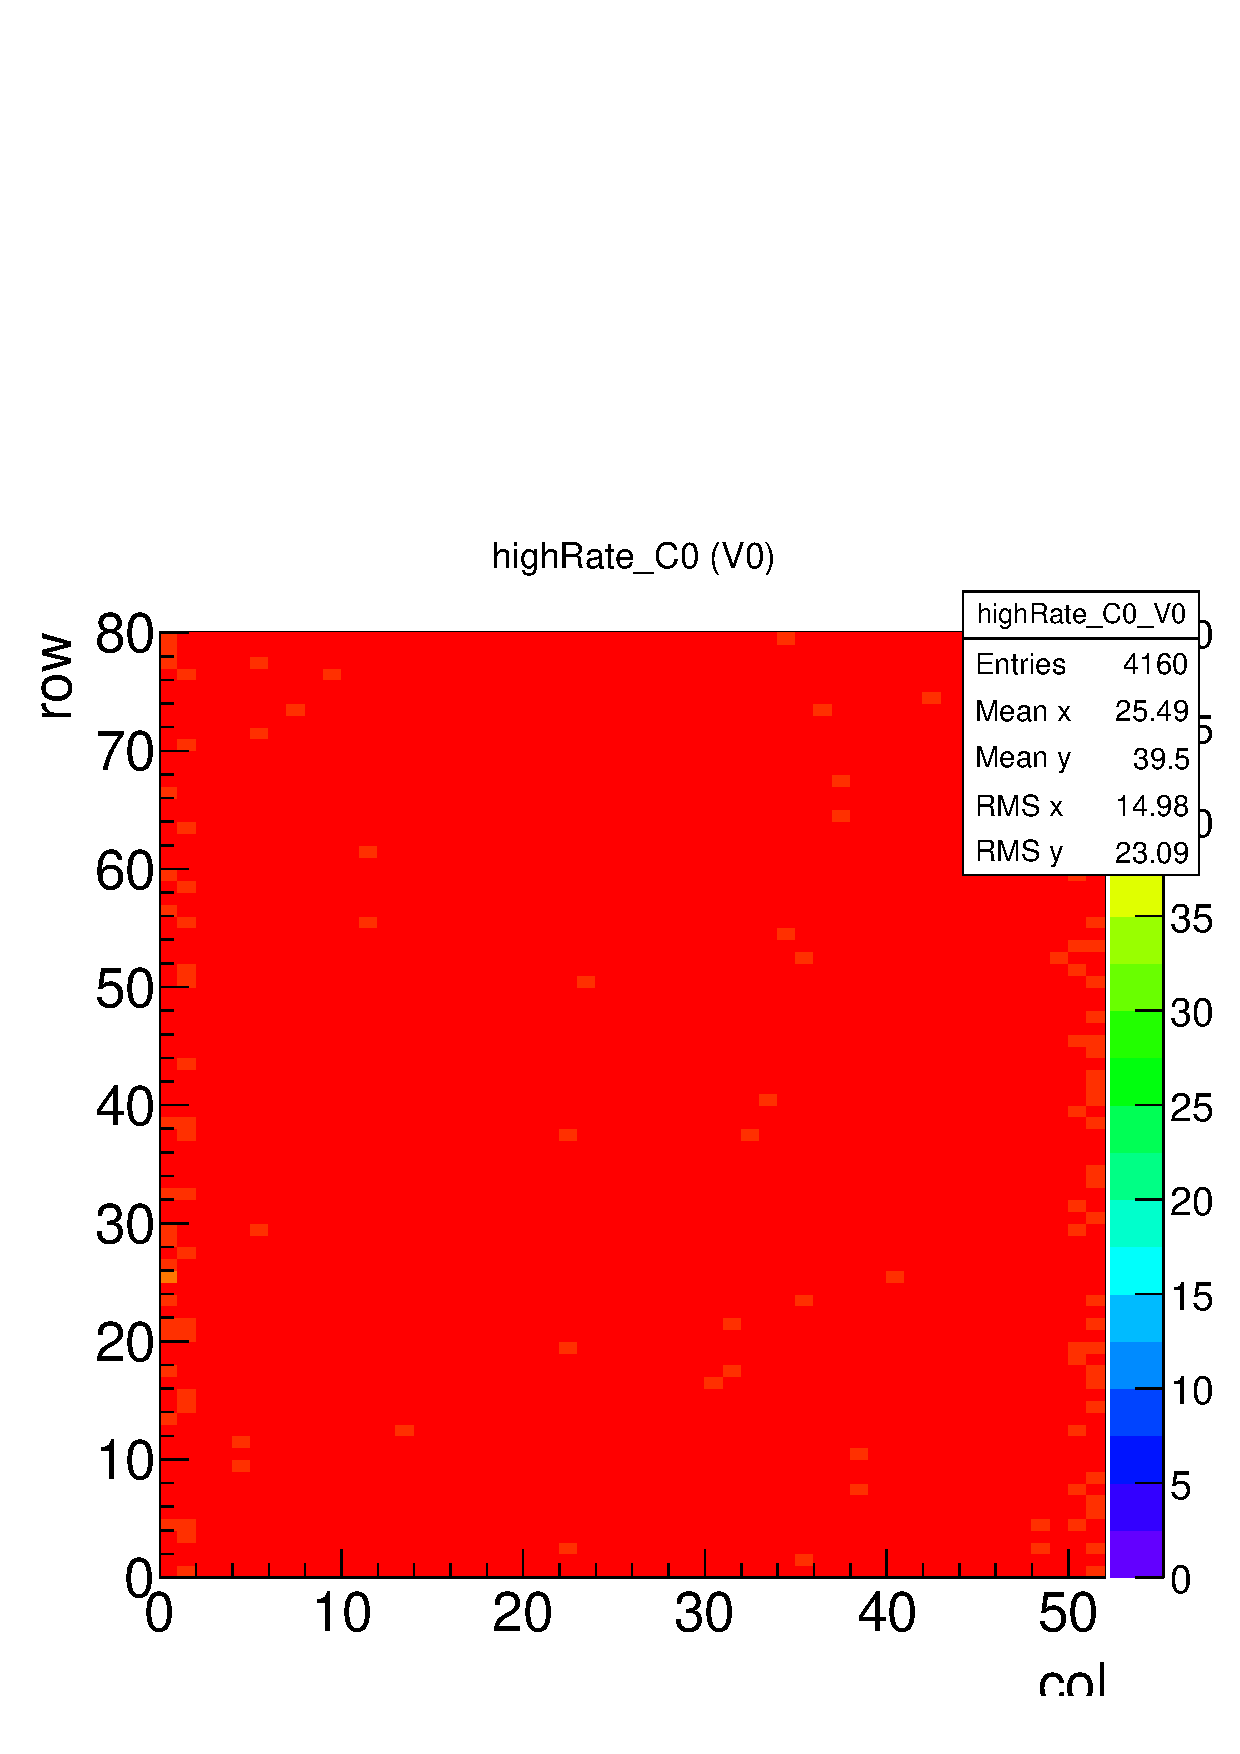
\includegraphics[width=\textwidth]{./Efficiency_Map.pdf}
  \captionof{figure}{Number of correctly read-out test pulses per pixel.}
  \label{Efficiency-Map}
\end{minipage}%
\hspace{2mm}
\begin{minipage}{.48\textwidth}
  \centering
  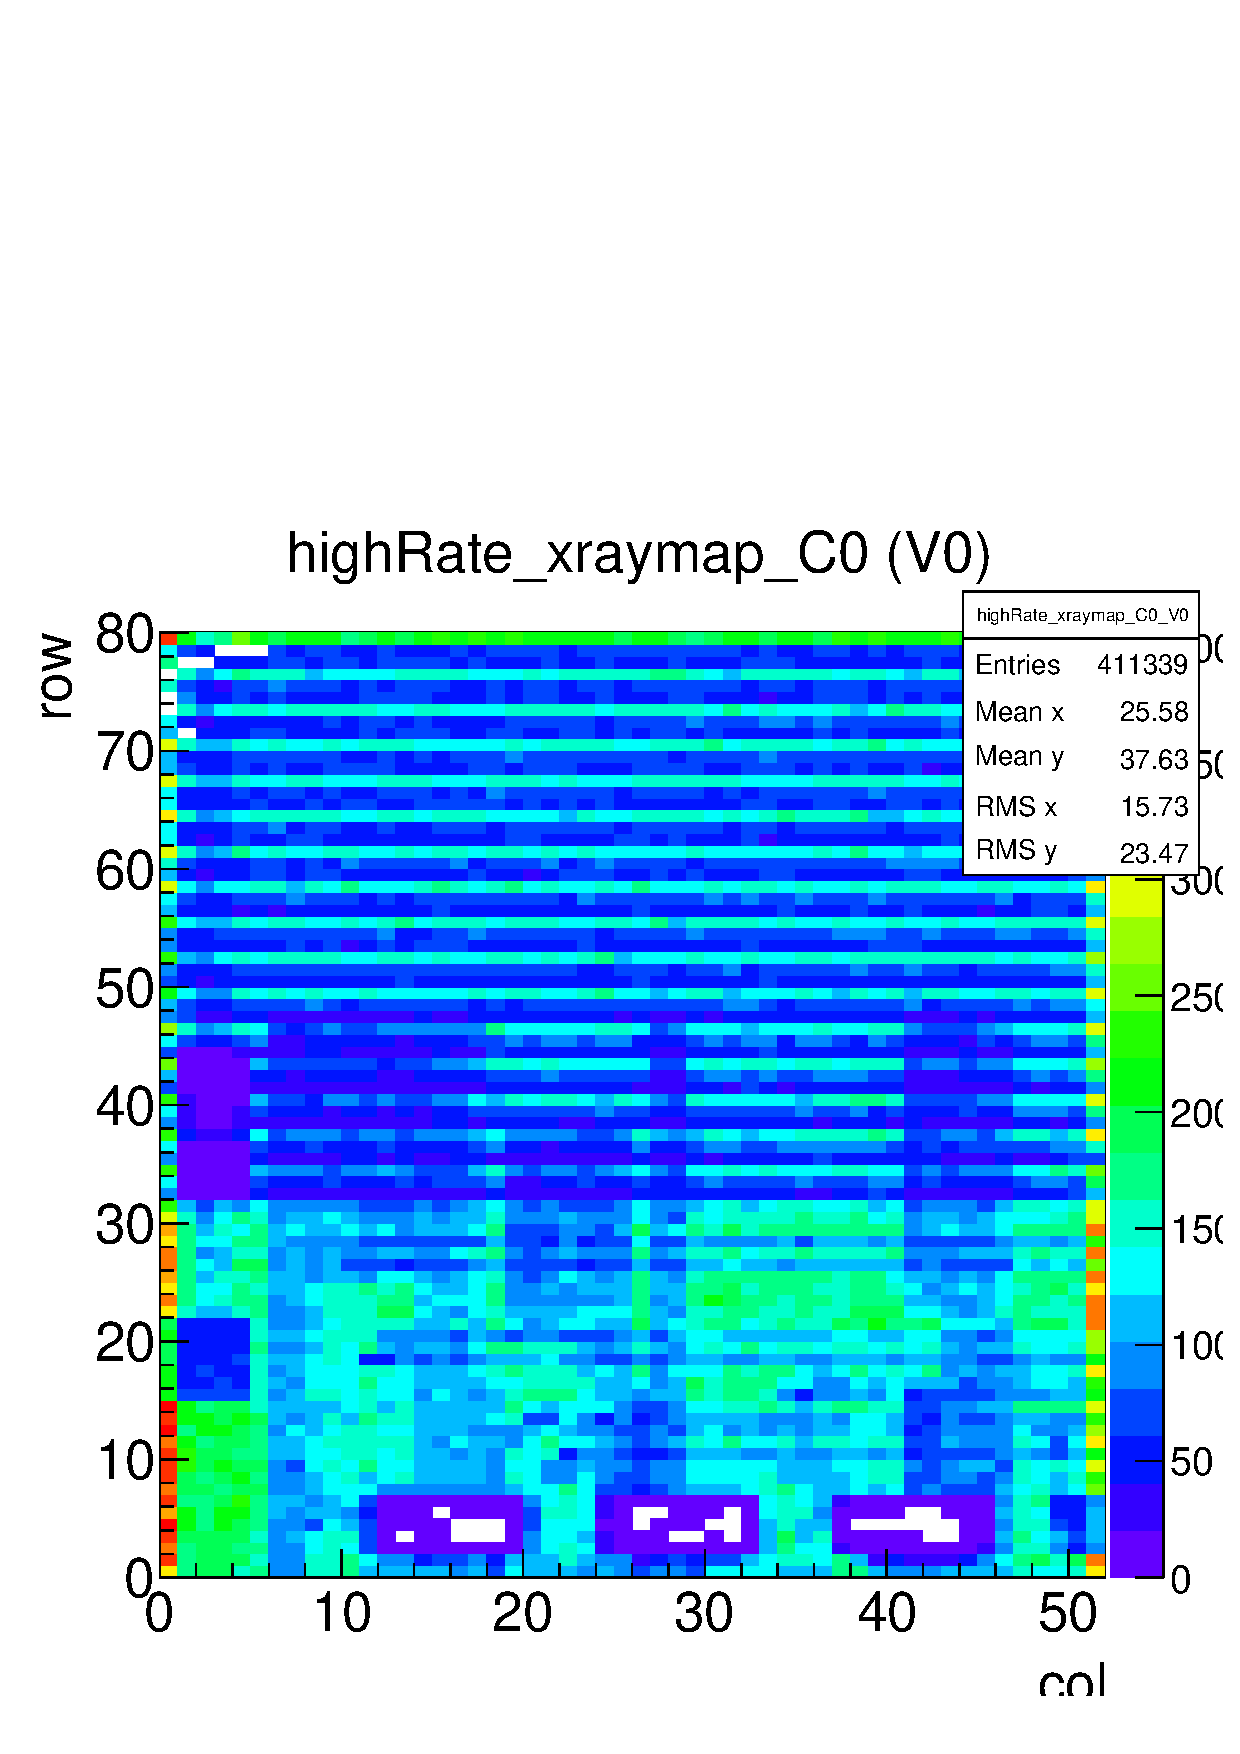
\includegraphics[width=\textwidth]{./Efficiency_BackgroundMap.pdf}
  \captionof{figure}{Hit map acquired during the efficiency measurement.}
  \label{Efficiency-Hitmap}
\end{minipage}
\end{figure}

\begin{figure} [h!]
\centering
\begin{minipage}{.48\textwidth}
  \centering
  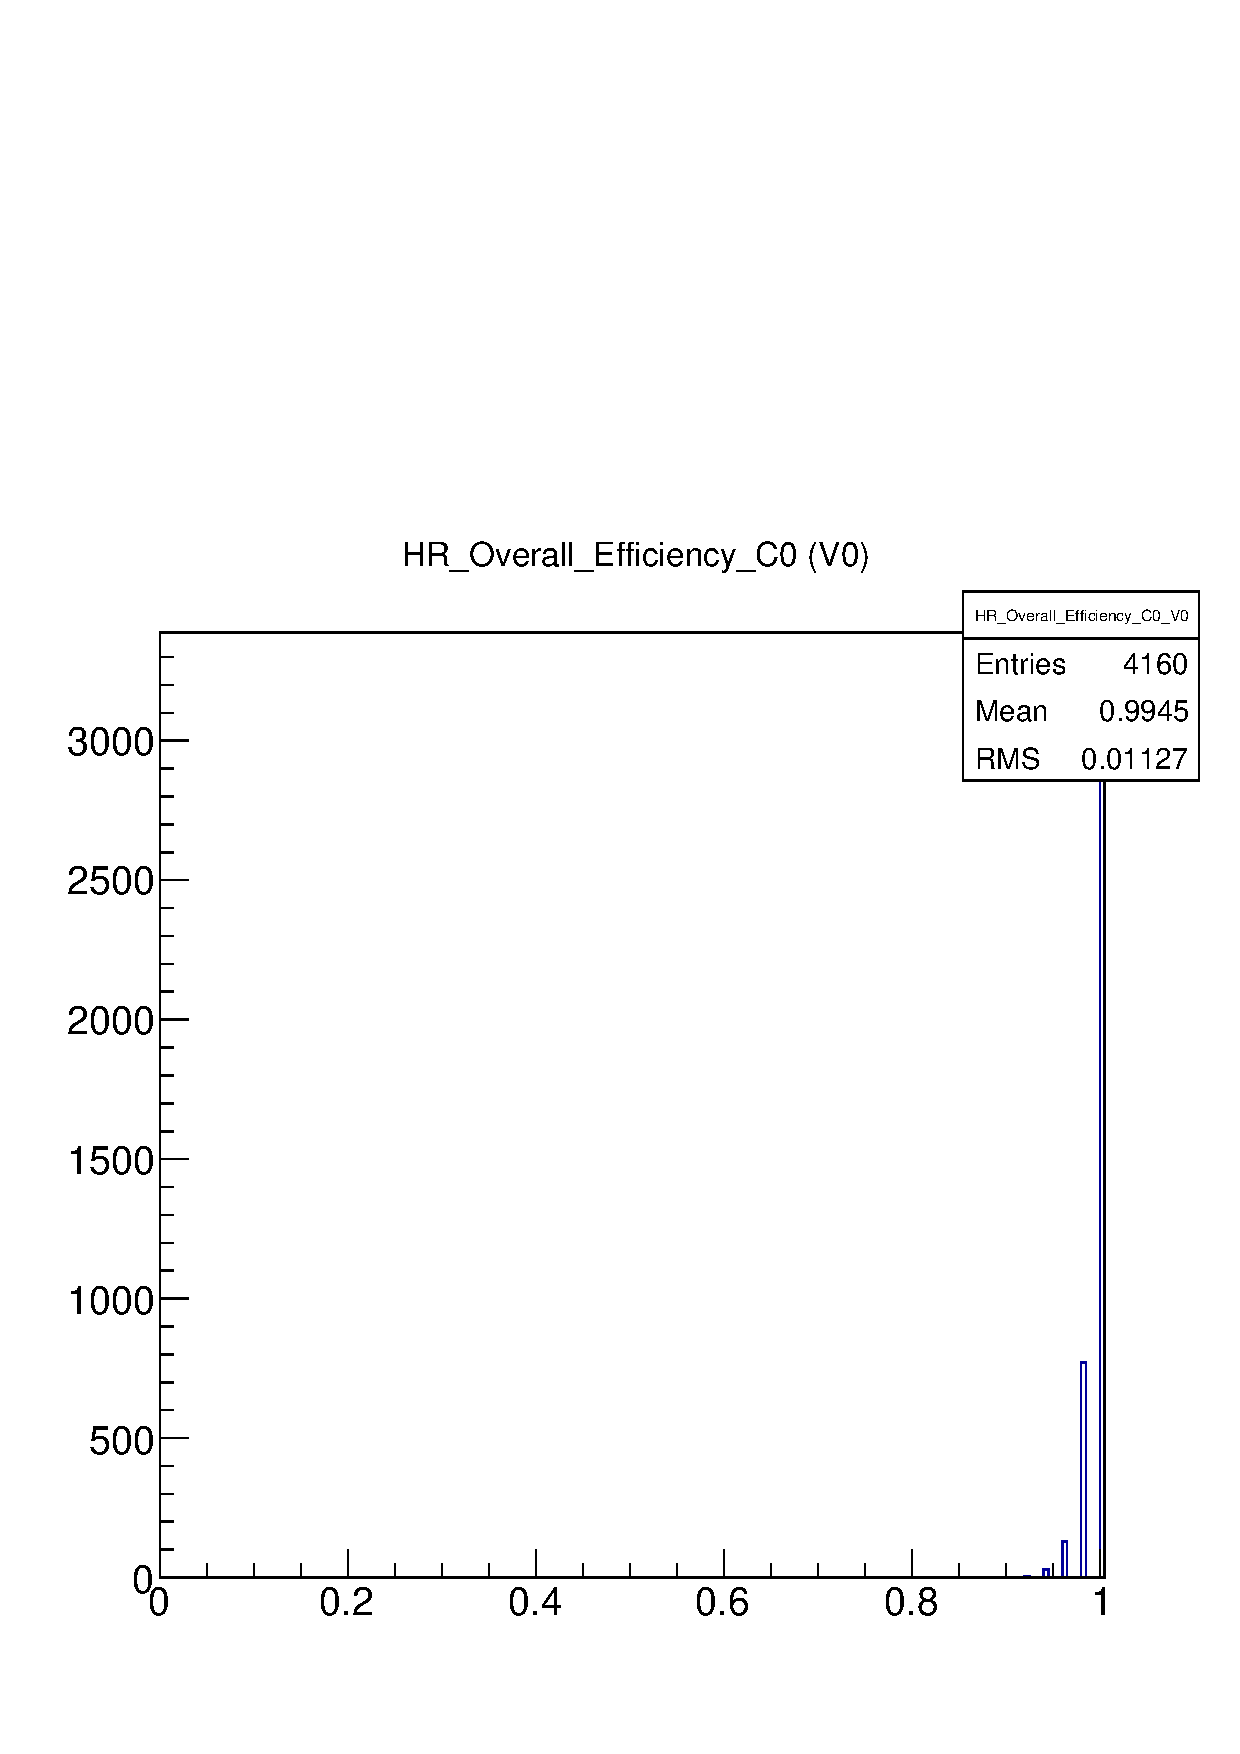
\includegraphics[width=\textwidth]{./Efficiency_Overall.pdf}
  \captionof{figure}{Efficiency distribution of all pixels}
  \label{Efficiency-Overall}
\end{minipage}%
\hspace{2mm}
\begin{minipage}{.48\textwidth}
  \centering
  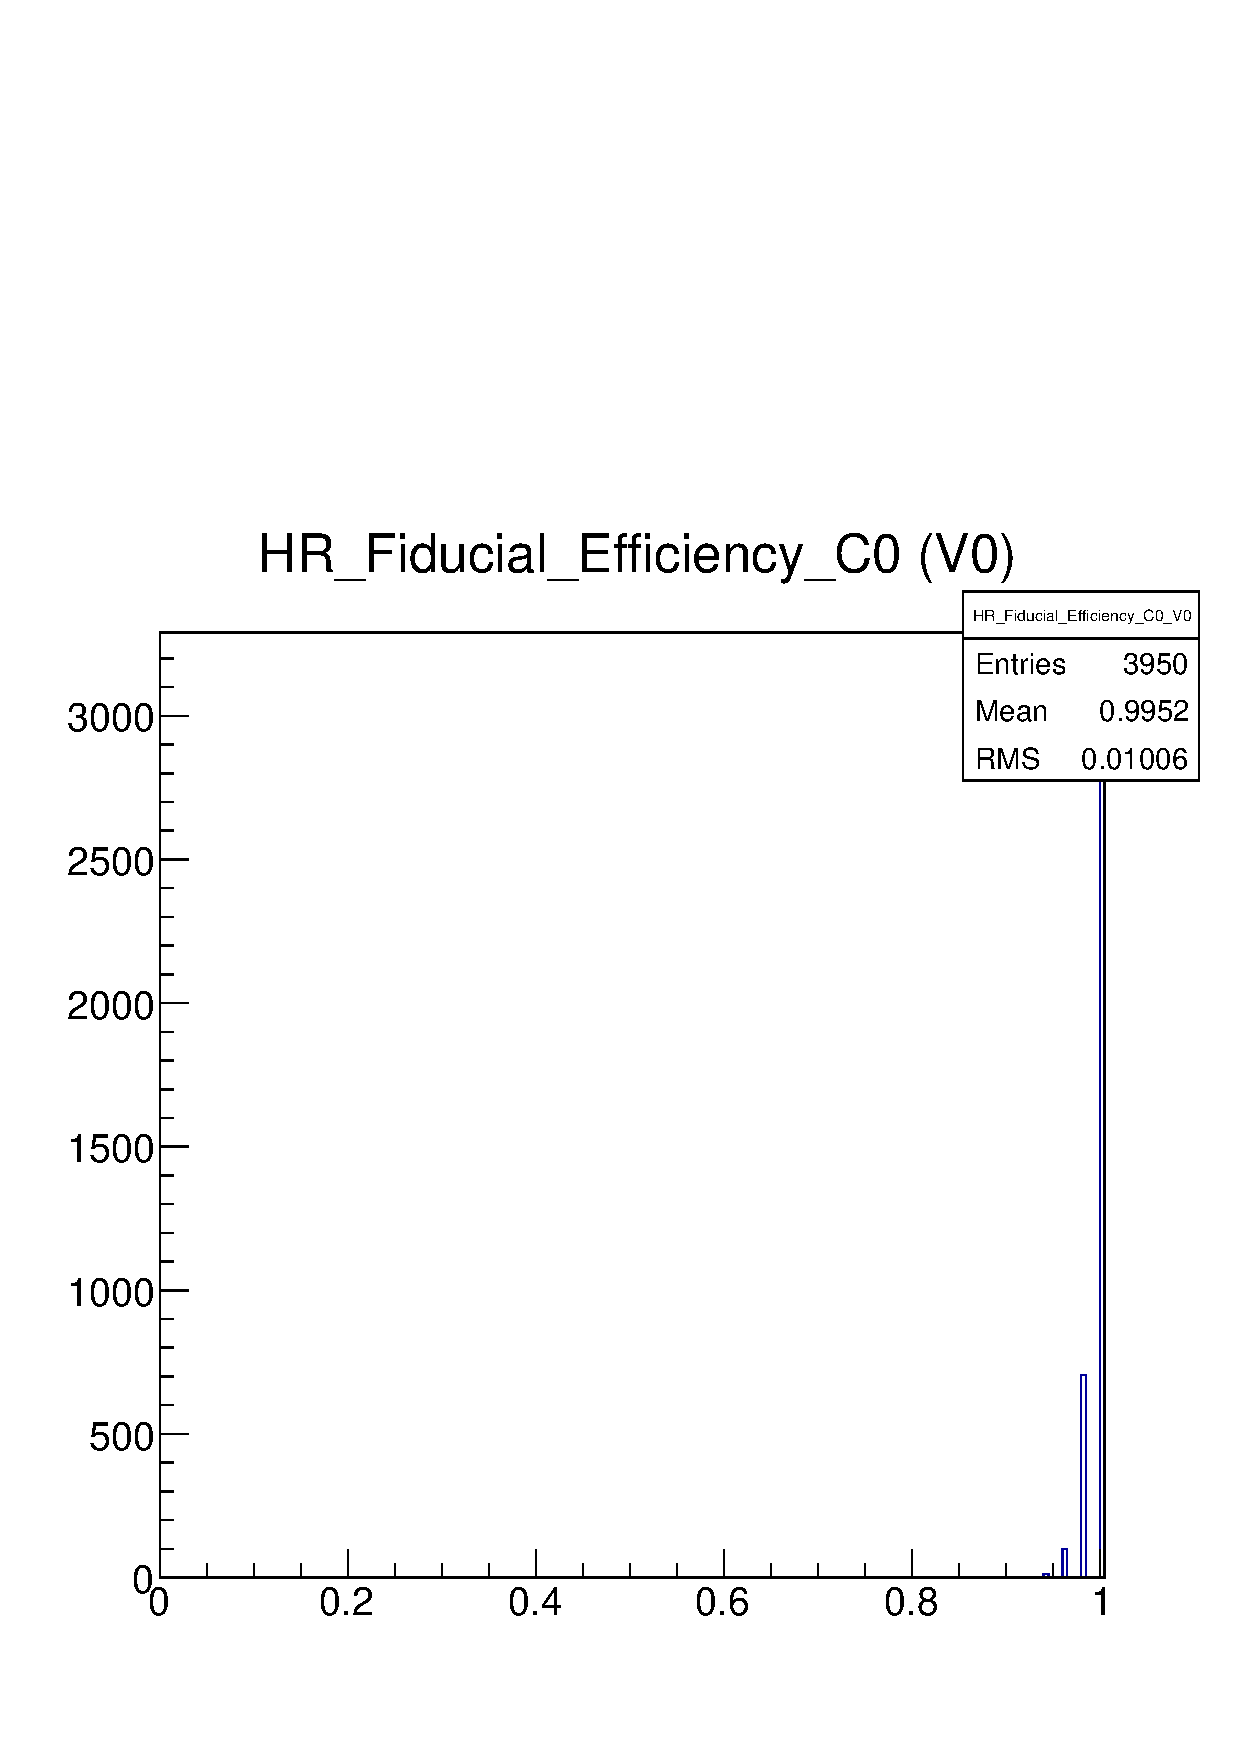
\includegraphics[width=\textwidth]{./Efficiency_Fiducial.pdf}
  \captionof{figure}{Efficiency of all pixels in the fiducial region (which excludes all edge pixels).}
  \label{Efficiency-Fiducial}
\end{minipage}
\end{figure}

This test is performed at different rates to measure the efficiency of each ROC. The test sends a set number of calibrate signals to each pixels while the chip is exposed to radiation. Evaluating the fraction of correctly read-out calibrate signals gives the efficiency. The hit rate at which this efficiency was measured is evaluated by counting the number of X-ray hits recorded, and is corrected for the calculated efficiency. Here, one assumes that the efficiency to detect both kinds of hits is the same which is a sensible assumption both type of hits go through the same read-out chain of the ROC.

\section{MoReWeb results of module qualification}

\subsection{XraySpectrum - Vcal Calibration}
The XraySpectrum test is performed with four scintillating targets so that a monochromatic X-ray beam reaches the module. This test enables to establish conversion parameters between a pulse height in ROC internal ADC units and electrons. This conversion is slightly different for all ROCs.

\section{Results}
\subsection{L2}
325 modules in total were tested in the X-ray qualification. Out of these, 242 received grade A, 39 grade B and 44 grade C, leading to a yield of 86.5\% (note that modules with severe defects that were discovered in the FQ are not tested in the X-ray qualification and do not appear in the results shown here). 

Most modules graded C in the X-ray qualification are due to DC defects which will be described later.


\begin{itemize}
\item Noise:
The noise of most pixels is unproblematic
\begin{figure} [h!] \centering 
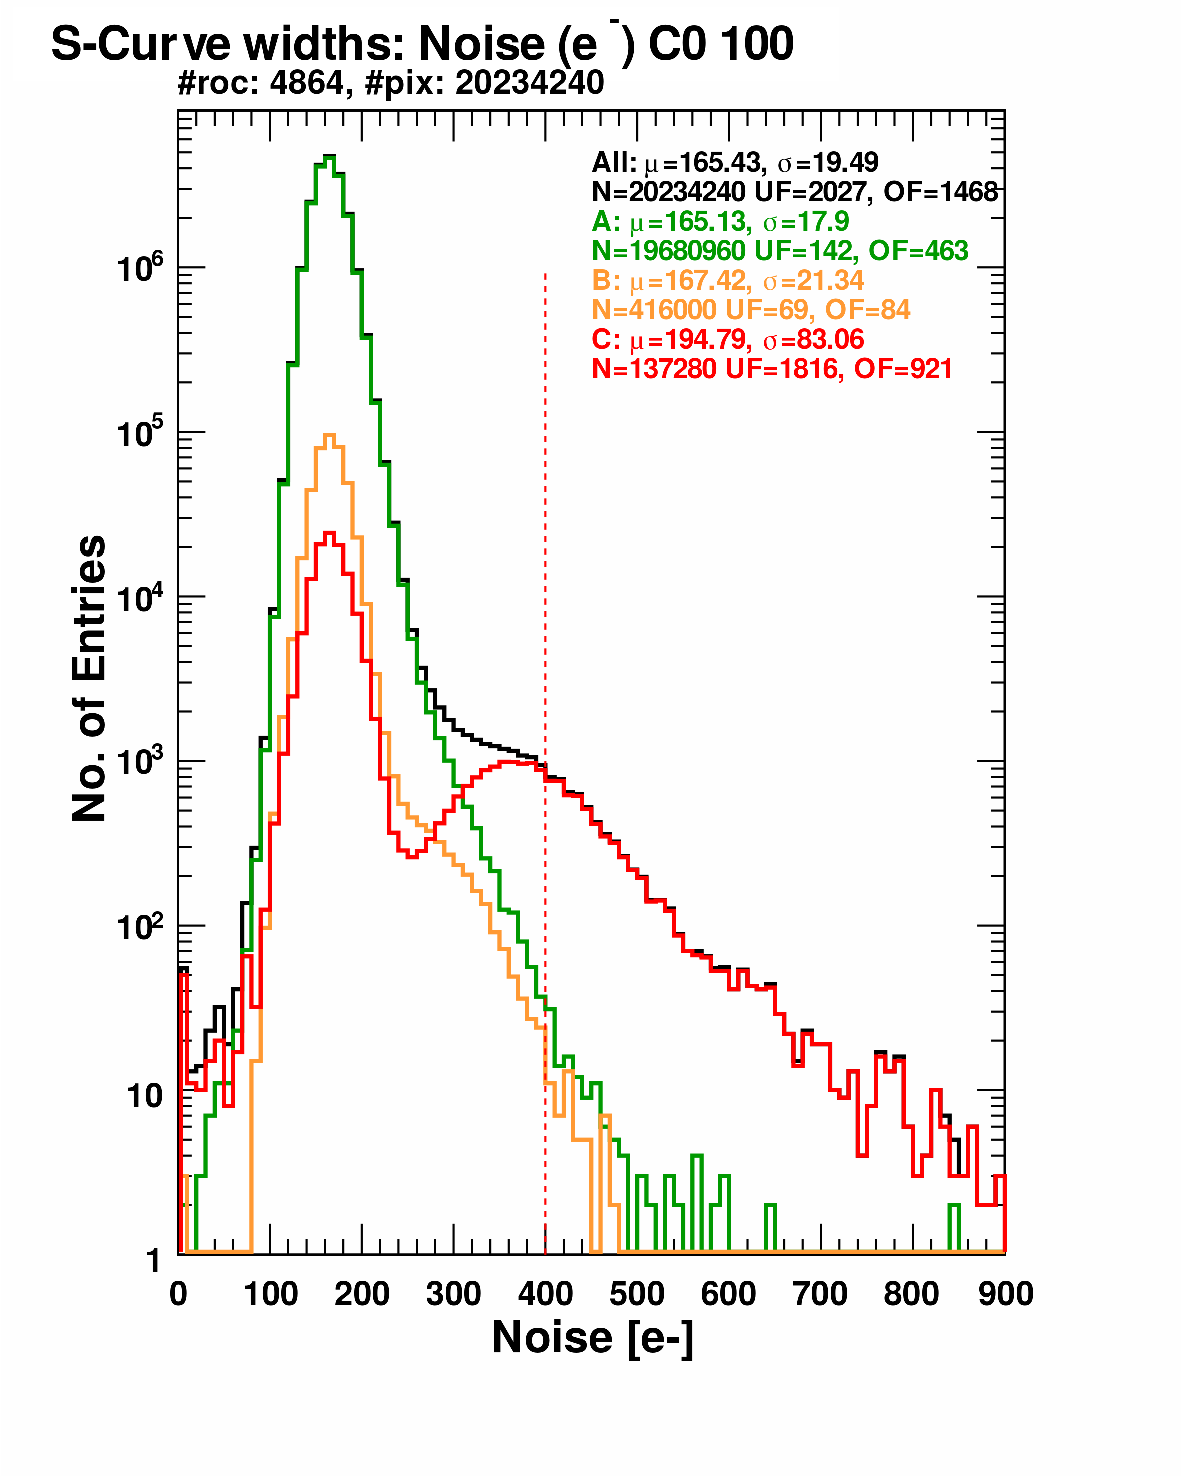
\includegraphics[width=0.4\textwidth, angle=0] {./Xray_NoisePerPixel.pdf}
\end{figure}

\begin{figure} [h!] \centering 
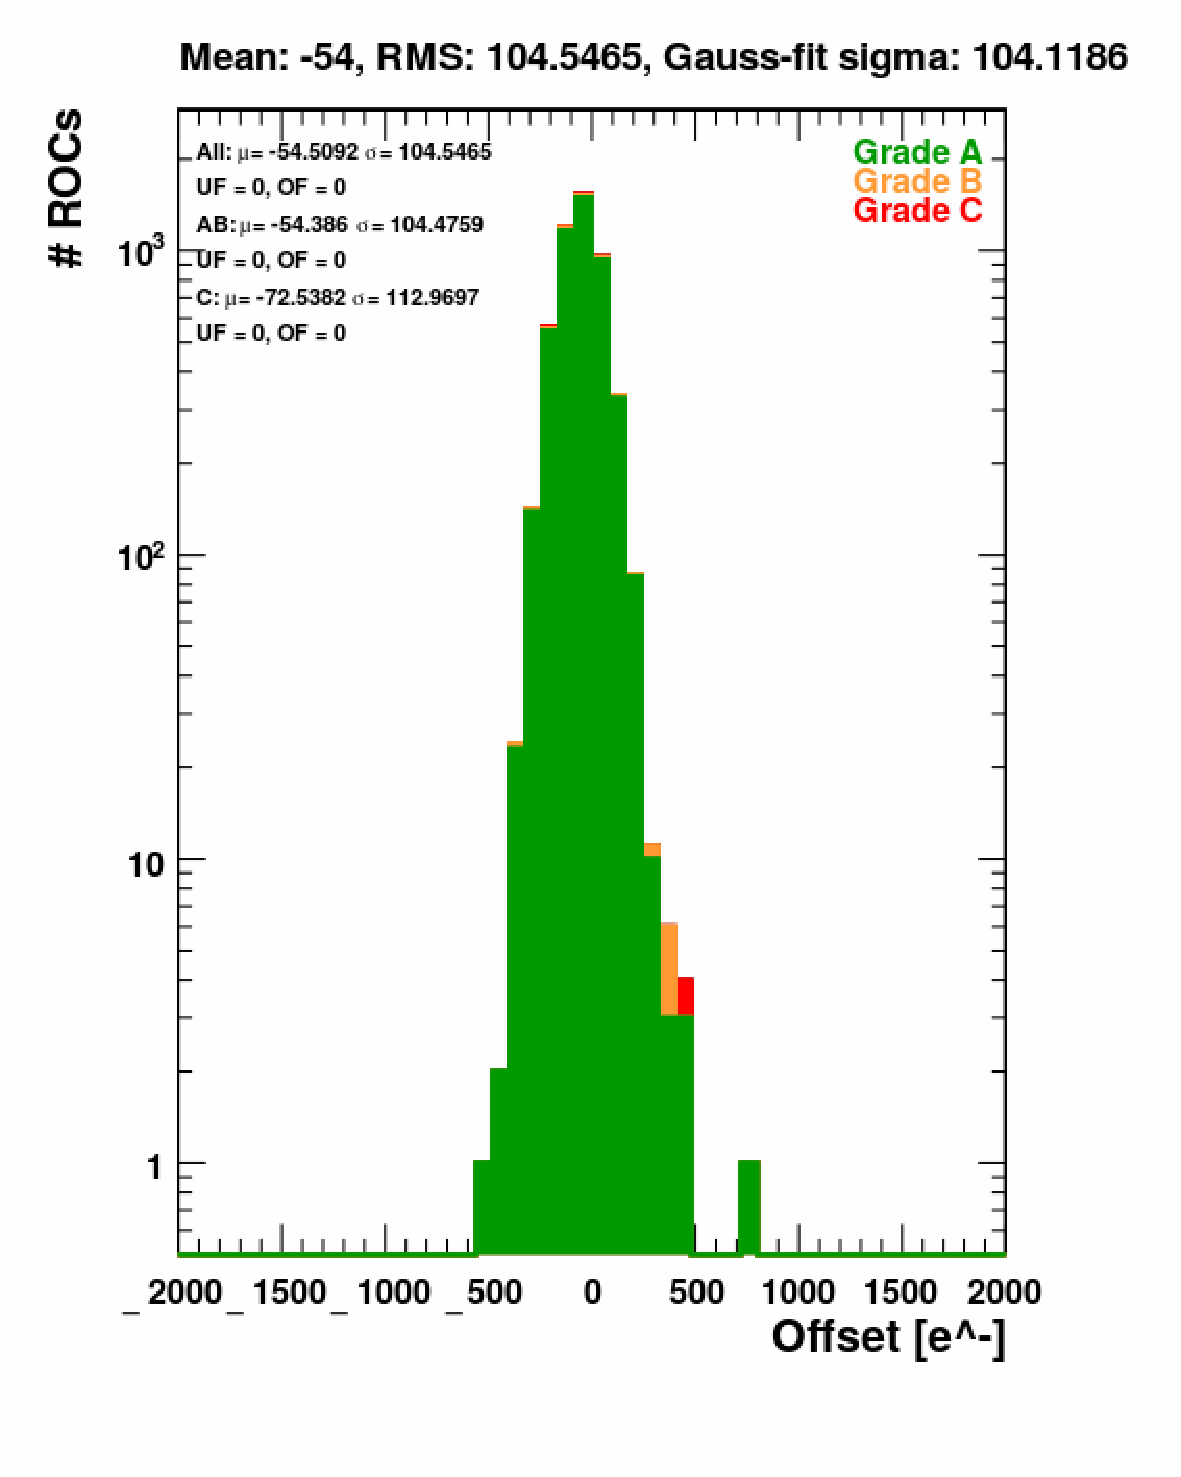
\includegraphics[width=0.4\textwidth, angle=0] {./Xray_VcalOffset.pdf}
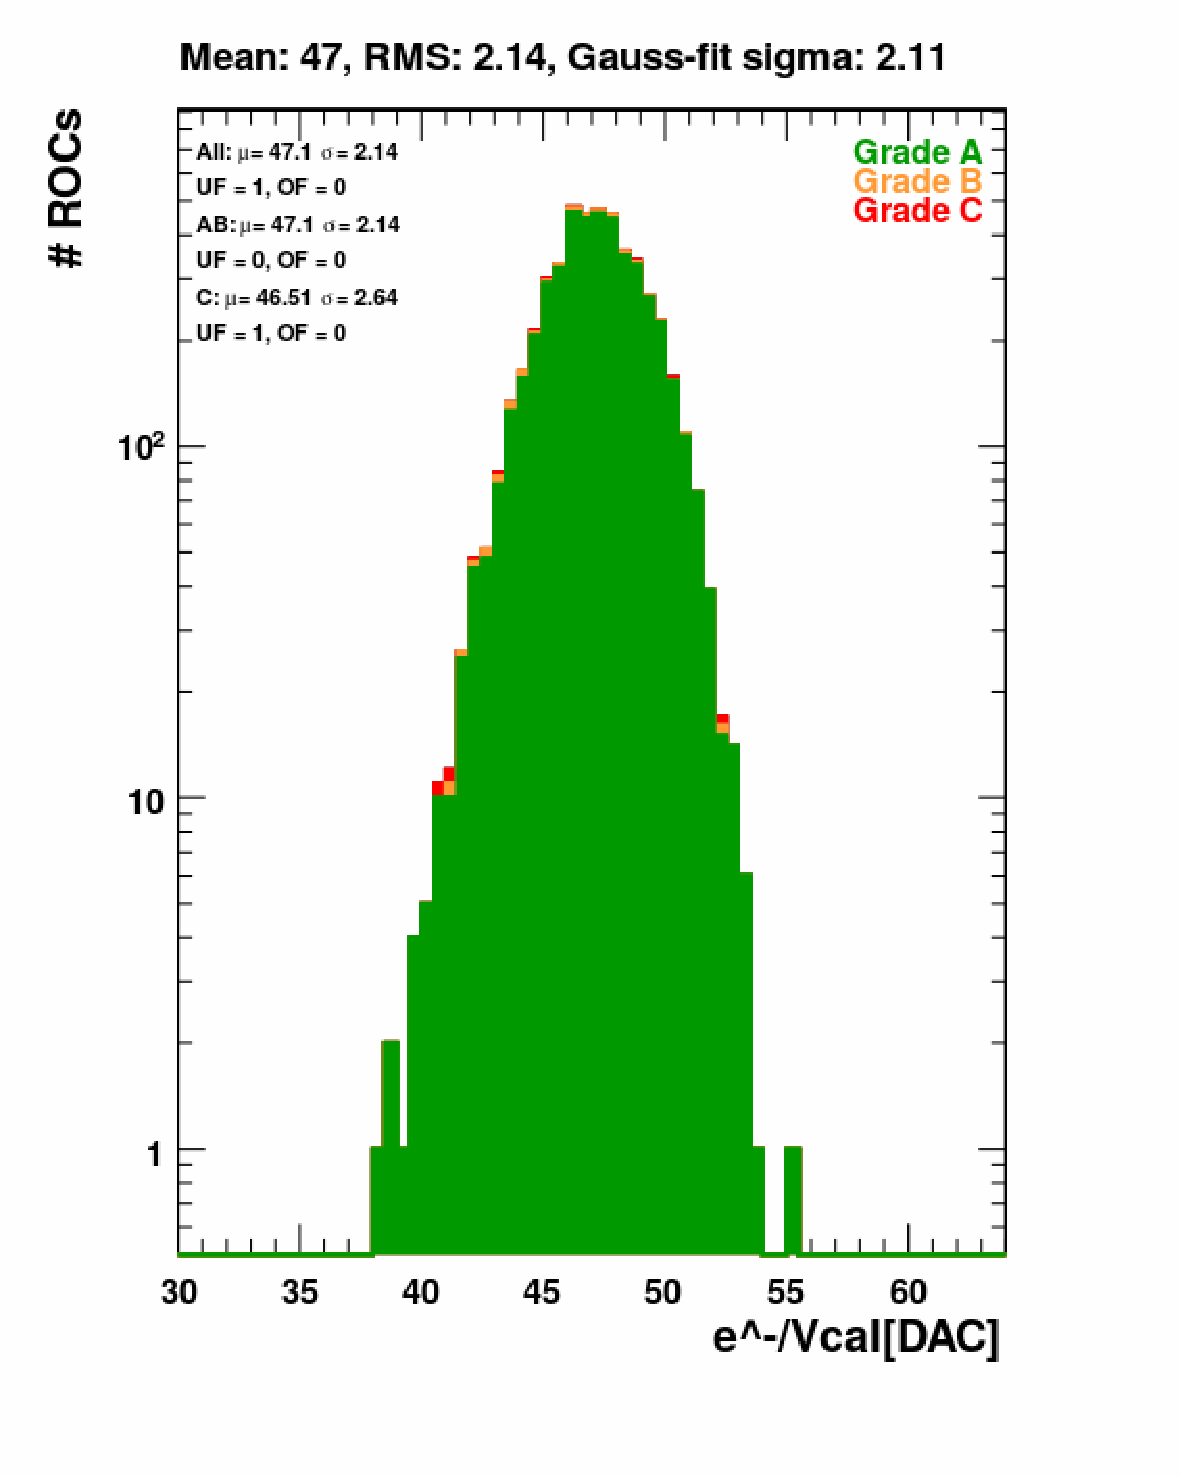
\includegraphics[width=0.4\textwidth, angle=0] {./Xray_VcalSlope.pdf}
\end{figure}

\begin{figure} [h!] \centering 
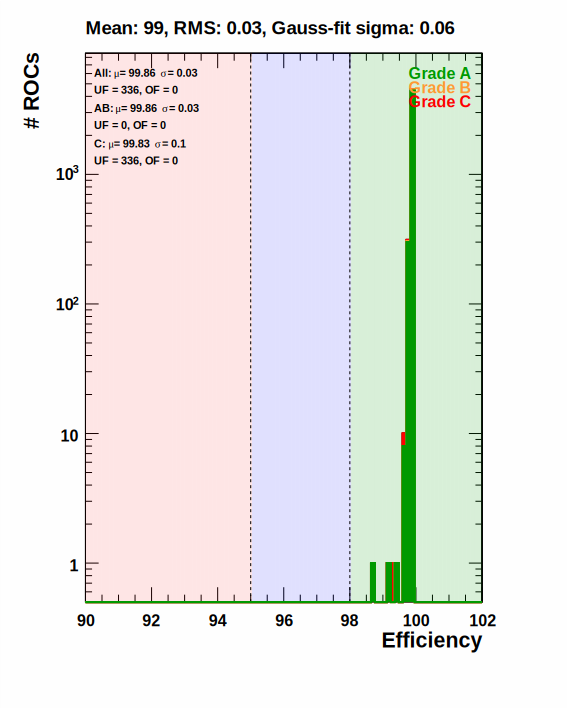
\includegraphics[width=0.4\textwidth, angle=0] {./Xray_Efficiency_50.pdf}
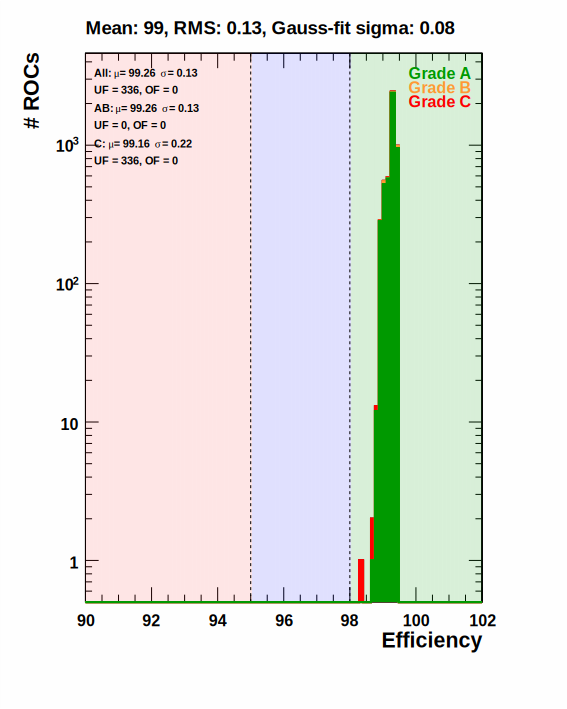
\includegraphics[width=0.4\textwidth, angle=0] {./Xray_Efficiency_120.pdf}
\end{figure}
\end{itemize}



\subsection{L1}
\subsection{Reasons for failure of the test}
The X-ray qualification was only performed with modules where no severe problems appeared in the Full Qualification, such as non programmable ROCs. These defects are therefore not listed here, but in the corresponding section on the FQ.
\subsubsection{Double-column defects}
Most of the modules failing the X-ray qualification are caused by a defective double-column on one or multiple ROCs. The problem is particularly noticeable for L1 modules (give percentages). The characteristics of these defects are very different. For some modules it can be noticed either on the hitmaps, or when calibrate signals are used, or sometimes also for both. These defects can sometimes also be recognized by an electrical DC test that verifies the functionality of data and timestamp buffers, but this is not the case for all modules. 
\subsection{BB defects}
Modules with too many BB defects also fail the X-ray qualification. These are usually already seen in the full qualification
\subsection{Other problems}
Though no module during the 2015/2016 production was downgraded due to this, the automatic grading in MoReWeb also considers the noise measured while exposing the module to radiation (only for L2), and the efficiency at the maximum expected rate for the corresponding layer. 

\begin{appendices}
%\appendix

\section{Replacement of Peltier elements in the climatic chamber} \label{Peltier}

These steps summarize the necessary work to replace a Peltier element in the X-ray set up.
\begin{itemize}
\item Unscrew the plate holding the temperature monitor (Shown on Picture~\ref{Commandboard} - careful, cables are attached to it).
\item Verify which Peltier elements are faulty by only connecting one Peltier at a time (see Figure~\ref{Step2}). If it is faulty, the Peltier element will not draw any current as seen on the power supply.
\item Remove water supplies and serial adapter from the right side of the climatic chamber.
\item Unscrew top frame (see Figure~\ref{Step4} - upper screws on the sides).
\item Remove front, back and right side panels (see Figure~\ref{Step5a} and \ref{Step5b}).
\item Remove cooling plate. The temperature sensor must be unplugged for this (see Figure~\ref{Step6}).
\item Unscrew Peltier element connector (see Figure~\ref{Step7}), unplug temperature sensor on copper block if access is needed to the Peltiers in the back.
\item Take out all the Peltier elements, remove the thermal grease, and replace the broken ones.
\item Apply thermal grease on the copper block at the dedicated spots, put the Peltiers on top (see Figure~\ref{Step9a} and \ref{Step9b}).
\item Reconnect the Peltier elements.
\item Put thermal grease on top of the Peltier elements.
\item Reconnect the temperature sensor.
\item Rescrew the cooling plate and all the other parts of the climatic chamber.

\end{itemize}
\begin{figure} [h!]
\centering
\begin{minipage}{.48\textwidth}
  \centering
  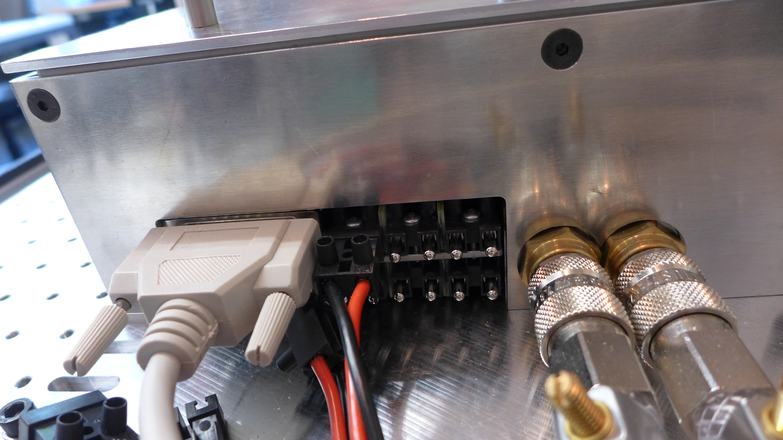
\includegraphics[width=\textwidth]{./Point2.png}
  \captionof{figure}{Verification of the functionality of the Peltier elements.}
  \label{Step2}
\end{minipage}%
\hspace{2mm}
\begin{minipage}{.48\textwidth}
  \centering
  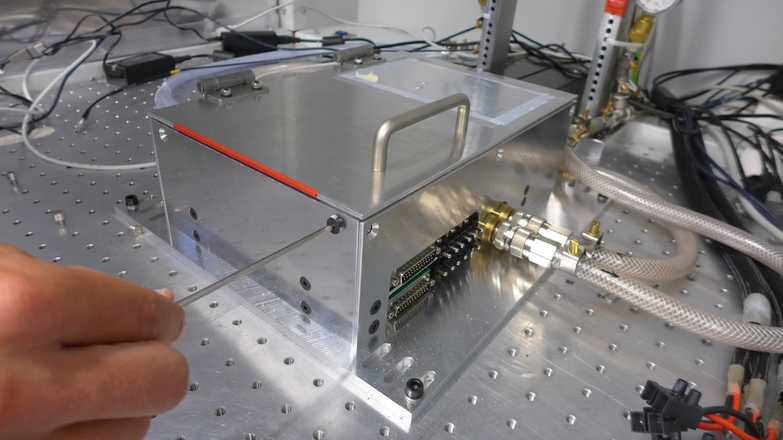
\includegraphics[width=\textwidth]{./Point4.png}
  \captionof{figure}{Unscrewing of the walls of the climatic chamber.}
  \label{Step4}
\end{minipage}
\end{figure}

\begin{figure} [h!]
\centering
\begin{minipage}{.48\textwidth}
  \centering
  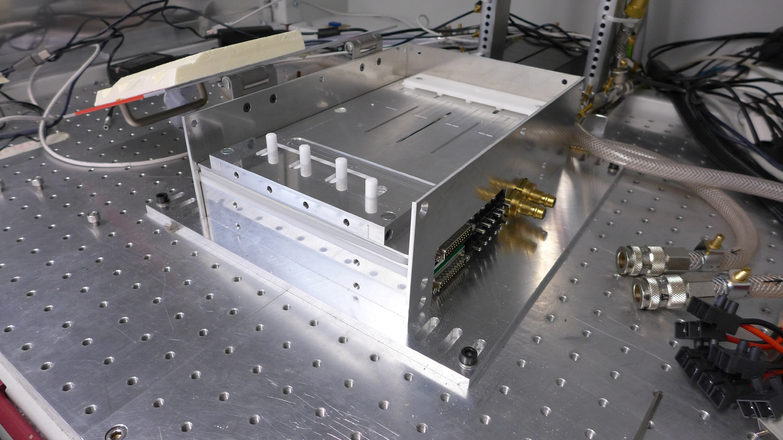
\includegraphics[width=\textwidth]{./Point5a.png}
  \captionof{figure}{Picture of the opened climatic chamber I.}
  \label{Step5a}
\end{minipage}%
\hspace{2mm}
\begin{minipage}{.48\textwidth}
  \centering
  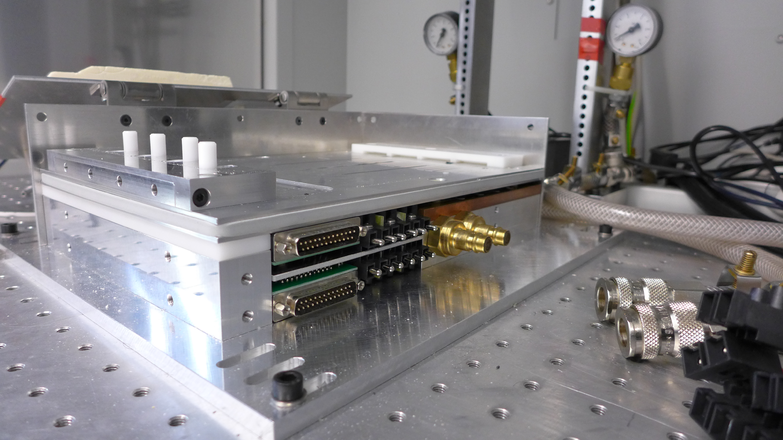
\includegraphics[width=\textwidth]{./Point5b.png}
  \captionof{figure}{Picture of the opened climatic chamber II.}
  \label{Step5b}
\end{minipage}
\end{figure}

\begin{figure} [h!]
\centering
\begin{minipage}{.48\textwidth}
  \centering
  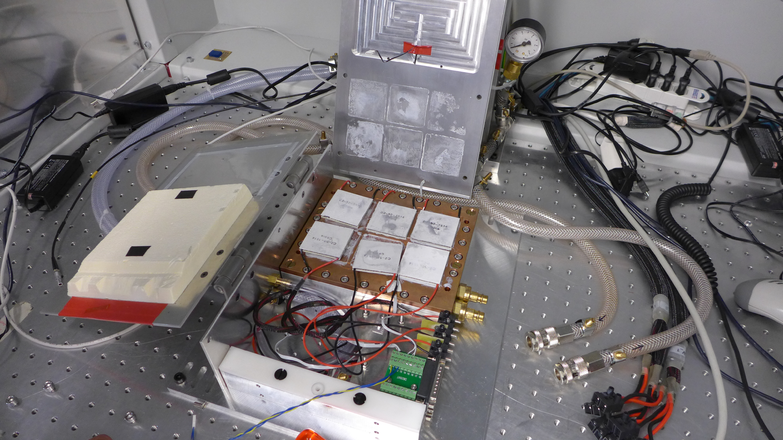
\includegraphics[width=\textwidth]{./Point6.png}
  \captionof{figure}{Picture of the climatic chamber with removed base plate.}
  \label{Step6}
\end{minipage}%
\hspace{2mm}
\begin{minipage}{.48\textwidth}
  \centering
  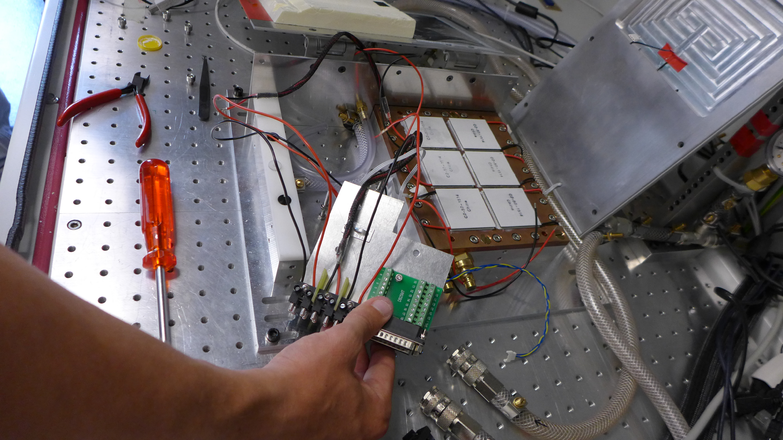
\includegraphics[width=\textwidth]{./Point7.png}
  \captionof{figure}{Picture of the Peltier element connector}
  \label{Step7}
\end{minipage}
\end{figure}

\begin{figure} [h!]
\centering
\begin{minipage}{.48\textwidth}
  \centering
  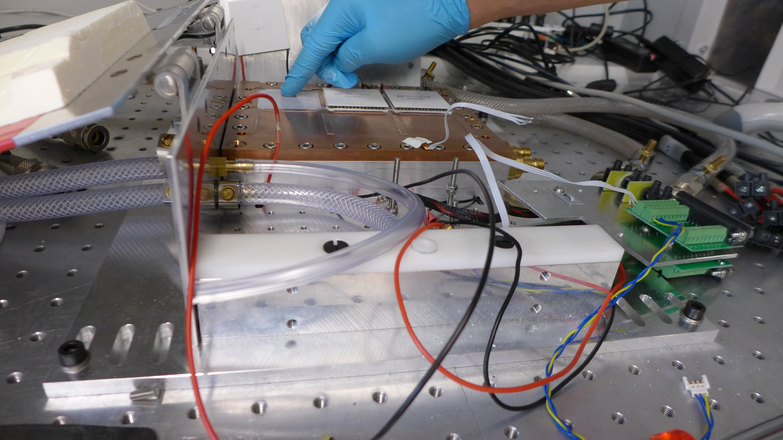
\includegraphics[width=\textwidth]{./Point9a.png}
  \captionof{figure}{Thermal grease application on the Peltier elements.}
  \label{Step9a}
\end{minipage}%
\hspace{2mm}
\begin{minipage}{.48\textwidth}
  \centering
  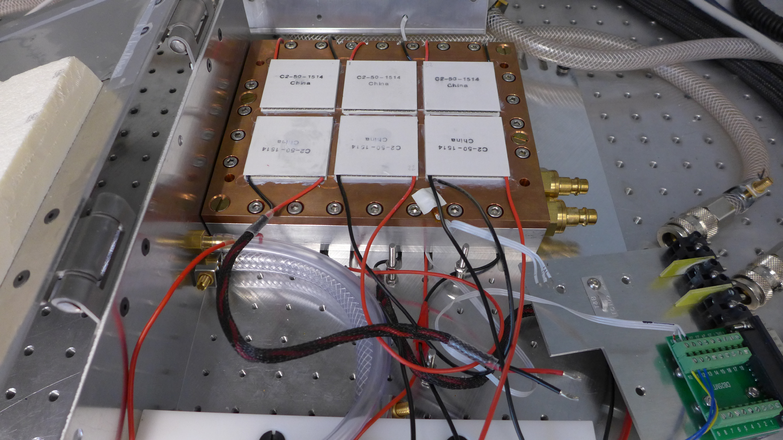
\includegraphics[width=\textwidth]{./Point9b.png}
  \captionof{figure}{Picture of all Peltier elements in the climatic chamber.}
  \label{Step9b}
\end{minipage}
\end{figure}
\clearpage
\newpage
\section{Cleaning of the X-ray filter} \label{Filter}

Before performing this operation, make sure that the dirty filter is actually the cause of the problem. To do this, turn ID3003 program off, hold the "Enter" button, turn the key to "Stand By" and select 2. Then select item 02 "Preset flow rate" which will show the water flow. It should be around \SI{6}{\litre\per\minute}. If the flow is below \SI{3.5}{\litre\per\minute}, the system will not start any more, and the filter has to be cleaned.
\\

\textbf{
WARNING:  \\
\\
Only unmount the tube if you know what you are doing. Read the manuals. This instruction alone does not qualify you for doing the operation. If you have doubts, call the reseller company Fisch and Partner! 
\\
\\
Handle tube carefully, do not touch beryllium windows. If they get wet, carefully dry them WITHOUT exerting force to them. Water on the windows causes them to corrode.
\\
\\
Beryllium is poisonous when in contact with skin and VERY brittle! Note that there are 4 windows in total.}

\begin{itemize}

\item Close water return and supply at the ceiling of the lab (in this order to prevent static pressure) and the inlet at the wall. Empty hoses by dis-attaching them far away from the set up and empty them in a bucket. Remove devices below x-ray tube as it may get wet.empty the tubes. 

\item Carefully unscrew the tube base plate from the mounting rack (2 big diagonal slotted screws) and catch the water which will start leaking out. The tube with the base plate is pressed towards the power connector in the back with a spring, one has to hold it and be careful otherwise if might pop out.

\item Pull out the tube very carefully without bumping it against the housing of the tube. The tube is at very low pressure and can implode if it breaks. Danger by flying shards! Place it in a safe place. It is fine to lay it onto the glass cylinder. Do not touch the beryllium windows, if they get wet, carefully dry them without exerting force to them (e.g. suck the water with the corner of a soft tissue. Detach the base plate from the tube by unscrewing 4 hex screws as shown in Figures~\ref{screws1} and \ref{screws2}. Two of these screws are hidden in the holes of the front plate. Figure~\ref{frontmountplate} shows the front plate which was unscrewed from the X-ray tube.

\item The filter is in a casing below on the base plate (see Figure~\ref{holder}). Remove the filter cap carefully (it has a $\sim 0.5 \times 10$\;\si{\milli\meter} slit on the top). Corrosion might make the cap stick to the baseplate. If needed, use two screw drivers to lever the cap off without harming the baseplate itself. Then remove the filter from the filter cap by carefully pressing it out e.g. with the blunt side of a cutter.

\item Clean filter with water and by blowing pressurized air against the flow direction (available e.g. in the workshop). Figures~\ref{dirty} and \ref{clean} show the filter before and after cleaning.

\item Place filter back into its casing, make sure that it is sitting at the end of the cap. Figure~\ref{filterholder} shows the filter and its casing.

\item Screw base plate to the tube. There is only one configuration where all 4 screws fit.

\item Make sure the tube housing is absolutely dry! Remember that you will apply 60 000 V to the tube. Flushing the volume with dry air can speed up the process.

\item Re-insert the tube including the base plate into the case. Again avoid any collision with the housing. It has to be pressed against the power connector. Tighten the 2 diagonal screws.

\item Evaluate the success of the operation by measuring the water flow again.

\end{itemize}

\begin{figure} [h!]
\centering
\begin{minipage}{.48\textwidth}
  \centering
  \includegraphics[width=\textwidth]{./dirty.png}
  \captionof{figure}{Picture of the filter before cleaning.}
  \label{dirty}
\end{minipage}%
\hspace{2mm}
\begin{minipage}{.48\textwidth}
  \centering
  \includegraphics[width=\textwidth]{./clean.png}
  \captionof{figure}{Picture of the filter after cleaning.}
  \label{clean}
\end{minipage}
\end{figure}

\begin{figure} [h!]
\centering
\begin{minipage}{.48\textwidth}
  \centering
  \includegraphics[width=\textwidth]{./screws1.png}
  \captionof{figure}{Unscrewing of screws that hold the front plate I.}
  \label{screws1}
\end{minipage}%
\hspace{2mm}
\begin{minipage}{.48\textwidth}
  \centering
  \includegraphics[width=\textwidth]{./screws2.png}
  \captionof{figure}{Unscrewing of screws that hold the front plate II.}
  \label{screws2}
\end{minipage}
\end{figure}

\begin{figure} [h!]
\centering
\begin{minipage}{.48\textwidth}
  \centering
  \includegraphics[width=\textwidth]{./frontmountplate.png}
  \captionof{figure}{Front mount plate detached from the X-ray tube.}
  \label{frontmountplate}
\end{minipage}%
\hspace{2mm}
\begin{minipage}{.48\textwidth}
  \centering
  \includegraphics[width=\textwidth]{./holder.png}
  \captionof{figure}{Casing of the filter removed from the X-ray tube.}
  \label{holder}
\end{minipage}
\end{figure}

\begin{figure} [h!] \centering 
\includegraphics[width=0.48\textwidth, angle=0] {./filterholder.png}
\caption{\em  \label{filterholder} 
Filter and its casing.}
\end{figure}

\section{ElCommandante configuration files}  \label{Config}
The only files that need to be modified are the config/elComandante.conf and the config/elComandante.ini files. The first of those is used to indicate which port is occupied by the different devices steered by elCommandante. In the second one, one should indicate details about which tests to execute and under which conditions (temperature, X-ray hit rate).
Please note that for readability reasons some lines are split into several lines. For testing, its needs to be written in one line
\subsection{L1}
elCommandante.ini:
\begin{Verbatim}[frame=single,fontsize=\footnotesize]
[ModuleType]
TB0 = M1106
TB1 = M1140
TB2 = -
TB3 = -

[Modules]
TB0 = M1106
TB1 = M1140
TB2 = M2358
TB3 = M2359

[CoolingBox]
CoolingBoxUse = False

[Cycle]
nCycles = 2
highTemp = 17
lowTemp = 15

[Environment 4mA25kV]
XrayCurrent = 4
XrayVoltage = 25
Temperature = 17
XrayTarget = None

[Environment 25MHz/cm2]
XrayCurrent = 3
XrayVoltage = 18
Temperature = 17
XrayTarget = None

[Environment 50MHz/cm2]
XrayCurrent = 5
XrayVoltage = 30
Temperature = 17
XrayTarget = None

[Environment 75MHz/cm2]
XrayCurrent = 7
XrayVoltage = 30
Temperature = 17
XrayTarget = None

[Environment 100MHz/cm2]
XrayCurrent = 10
XrayVoltage = 30
Temperature = 17
XrayTarget = None

[Environment 125MHz/cm2]
XrayCurrent = 12
XrayVoltage = 30
Temperature = 17
XrayTarget = None

[Environment 150MHz/cm2]
XrayCurrent = 15
XrayVoltage = 30
Temperature = 17
XrayTarget = None

[Environment 175MHz/cm2]
XrayCurrent = 17
XrayVoltage = 30
Temperature = 17
XrayTarget = None

[Environment 200MHz/cm2]
XrayCurrent = 20
XrayVoltage = 30
Temperature = 17
XrayTarget = None

[Environment 225MHz/cm2]
XrayCurrent = 22
XrayVoltage = 30
Temperature = 17
XrayTarget = None

[Environment 250MHz/cm2]
XrayCurrent = 25
XrayVoltage = 30
Temperature = 17
XrayTarget = None

[Environment 300MHz/cm2]
XrayCurrent = 30
XrayVoltage = 30
Temperature = 17
XrayTarget = None

[Environment 400MHz/cm2]
XrayCurrent = 30
XrayVoltage = 34
Temperature = 17
XrayTarget = None

[Environment 500MHz/cm2]
XrayCurrent = 30
XrayVoltage = 40
Temperature = 17
XrayTarget = None

[Environment Ag]
XrayCurrent = <!Environment Xrf|XrayCurrent!>
Temperature = <!Environment Xrf|Temperature!>
XrayVoltage = <!Environment Xrf|XrayVoltage!>
XrayTarget = Ag

[Environment Ba]
XrayCurrent = <!Environment Xrf|XrayCurrent!>
Temperature = <!Environment Xrf|Temperature!>
XrayVoltage = <!Environment Xrf|XrayVoltage!>
XrayTarget = Ba

[Environment Br]
XrayCurrent = <!Environment Xrf|XrayCurrent!>
Temperature = <!Environment Xrf|Temperature!>
XrayVoltage = <!Environment Xrf|XrayVoltage!>
XrayTarget = Br

[Environment Cu]
XrayCurrent = <!Environment Xrf|XrayCurrent!>
Temperature = <!Environment Xrf|Temperature!>
XrayVoltage = <!Environment Xrf|XrayVoltage!>
XrayTarget = Cu

[Environment Fe]
XrayCurrent = <!Environment Xrf|XrayCurrent!>
Temperature = <!Environment Xrf|Temperature!>
XrayVoltage = <!Environment Xrf|XrayVoltage!>
XrayTarget = Fe

[Environment Mo]
XrayCurrent = <!Environment Xrf|XrayCurrent!>
Temperature = <!Environment Xrf|Temperature!>
XrayVoltage = <!Environment Xrf|XrayVoltage!>
XrayTarget = Mo

[Environment Sn]
XrayCurrent = <!Environment Xrf|XrayCurrent!>
Temperature = <!Environment Xrf|Temperature!>
XrayVoltage = <!Environment Xrf|XrayVoltage!>
XrayTarget = Sn

[Environment Zn]
XrayCurrent = <!Environment Xrf|XrayCurrent!>
Temperature = <!Environment Xrf|Temperature!>
XrayVoltage = <!Environment Xrf|XrayVoltage!>
XrayTarget = Zn

[Environment Xrf]
XrayCurrent = 30
Temperature = 17
XrayVoltage = 60
XrayTarget = Mo

[IV]
Delay = 2
Step = 10
Stop = -200
Start = 0

[Keithley]
BiasVoltage = -150
KeithleyUse = True

[LeakageCurrent]
Duration = 60

[LowVoltage]
LowVoltageUse = False

[OperationDetails]
Operator = production
Hostname = toblerone.ethz.ch
TestCenter = ETHZ

[Test HREfficiency]
testParameters = Ntrig=50

[Test PhOptimitation]
testParameters = saturationvcal=100

[Test Trim]
testParameters = Vcal=80

[Test XraySpectrum]
testParameters = runseconds=30

[TestboardUse]
TB0 = True
TB1 = True
TB2 = False
TB3 = False

[Test HRData]
testParameters = runseconds=20

[Test HRSCurves]
testParameters = DacLo=15,DacHi=75,Ntrig=50

[Test RetrimHotPixels]
testParameters = trimhotpixelthr=200,runsecondsHotPixels=1,savetrimbits=1 \
,maskuntrimmable=1

[Test RetrimHotPixelsNoRate]
testParameters = trimhotpixelthr=10,runsecondsHotPixels=5,savetrimbits=1 \
,maskuntrimmable=1

[Test Scurves]
testParameters = ntrig=50,DAC=vcal,DacLo=25,DacHi=150,dumpOutputFile=1 \
,dumpProblematic=1

[Tests]
Test = PixelAlive@17>IncreaseEdgeThr@17>RetrimHotPixels@150MHz/cm2> \
RetrimHotPixels@50MHz/cm2>{HRData@100MHz/cm2,HRData@300MHz/cm2, \
HRSCurves@250MHz/cm2,CalDelScanAndSaveDacs@100MHz/cm2>  \
{HREfficiency@50MHz/cm2,HREfficiency@100MHz/cm2,HREfficiency@150MHz/cm2, \
HREfficiency@200MHz/cm2,HREfficiency@250MHz/cm2,HREfficiency@300MHz/cm2, \
HREfficiency@400MHz/cm2}}
TestDescription = XrayQualification

[Xray]
XrayUse = True

[VerifyTestParameters]
CheckExistence = False

[BarcodeReader]
BarcodeReaderUse = True
Fill = Both
CorrectModuleNames = True

[Alerts]
AlertsUse = True

[VerifyDACs]
dacs = vicolor==100,phscale>0,phoffset>0,vcolorbias==100,ctrlreg==16,vdig==8

[PostProcessing]
run = /usr/local/data/clean_xray_folder.py -f -d {directory}

\end{Verbatim} 

elCommandante.conf:
\begin{Verbatim}[frame=single,fontsize=\footnotesize]
[defaultParameters]
M3501 = M3501
M3502 = M3502
M3503 = M3503
M3504 = M3504

[Directories]
baseDir = ../
testDefinitions = $configDir$/tests/
moduleDB = <!Directories|baseDir!>/moduleDB/
subserverDir = <!Directories|baseDir!>/subserverDATA/
dataDir = /usr/local/data/
jumoDir = <!Directories|baseDir!>/coolingBox/
keithleyDir = <!Directories|baseDir!>/keithleyClient/
defaultParameters = /home/production/pxarL1/data
scriptDir = <!Directories|baseDir!>/analysisClient/scripts/

[TestboardAddress]
TB0 = DTB_WWXJGB
TB1 = DTB_WWV6Z5
TB2 = DTB_WWXTQT
TB3 = DTB_WWV6Z5

[subsystem]
Ziel = 127.0.0.1
Port = 12334
coolingBoxSubscription = /jumo
keithleySubscription = /keithley
psiSubscription = /psi
xraySubscription = /xray
analysisSubscription = /analysis

[jumoClient]
port = /dev/ttyJUMO
programName = coolingBoxClient.py

[keithleyClient]
port = /dev/ttyUSB1

[lowVoltageClient]
lowVoltageType = yoctorelay

[xrayClient]
xrayDevice = /dev/ttyID3003
xrayType = id3003
xrfDevice = /dev/ttyZaber
xrfType = zaber
xrfTargets = Zn:0,Cu:25320,Mo:50640,Ag:75960,Sn:101280,Ba:126600,Br:151920
turnOffHV = False
beamOffBetweenTests = False

[psiClient]
psiVersion = /home/production/pxarL1/bin/pXar

[Transfer]
host = cmspixel.pi.infn.it
port = 23481
destination = /home/eth/dropbox
user = eth
checkForTars = False

\end{Verbatim}

\subsection{L2}
elCommandante.ini:
\begin{Verbatim}[frame=single,fontsize=\footnotesize]
[ModuleType]
TB0 = M2241
TB1 = M2246
TB2 = M2243
TB3 = M2245

[Modules]
TB0 = M2241
TB1 = M2246
TB2 = M2243
TB3 = M2245

[CoolingBox]
CoolingBoxUse = False

[Cycle]
nCycles = 2
highTemp = 17
lowTemp = 15

[Environment 4mA25kV]
XrayCurrent = 4
XrayVoltage = 25
Temperature = 17
XrayTarget = None

[Environment 25MHz/cm2]
XrayCurrent = 3
XrayVoltage = 18
Temperature = 17
XrayTarget = None

[Environment 50MHz/cm2]
XrayCurrent = 6
XrayVoltage = 18
Temperature = 17
XrayTarget = None

[Environment 75MHz/cm2]
XrayCurrent = 7
XrayVoltage = 20
Temperature = 17
XrayTarget = None

[Environment 100MHz/cm2]
XrayCurrent = 8
XrayVoltage = 22
Temperature = 17
XrayTarget = None

[Environment 125MHz/cm2]
XrayCurrent = 9
XrayVoltage = 23
Temperature = 17
XrayTarget = None

[Environment 150MHz/cm2]
XrayCurrent = 10
XrayVoltage = 24
Temperature = 17
XrayTarget = None

[Environment 175MHz/cm2]
XrayCurrent = 11
XrayVoltage = 25
Temperature = 17
XrayTarget = None

[Environment 200MHz/cm2]
XrayCurrent = 12
XrayVoltage = 26
Temperature = 17
XrayTarget = None

[Environment 225MHz/cm2]
XrayCurrent = 13
XrayVoltage = 27
Temperature = 17
XrayTarget = None

[Environment 250MHz/cm2]
XrayCurrent = 15
XrayVoltage = 26
Temperature = 17
XrayTarget = None

[Environment 300MHz/cm2]
XrayCurrent = 18
XrayVoltage = 26
Temperature = 17
XrayTarget = None

[Environment 400MHz/cm2]
XrayCurrent = 24
XrayVoltage = 26
Temperature = 17
XrayTarget = None

[Environment 500MHz/cm2]
XrayCurrent = 30
XrayVoltage = 26
Temperature = 17
XrayTarget = None

[Environment Ag]
XrayCurrent = <!Environment Xrf|XrayCurrent!>
Temperature = <!Environment Xrf|Temperature!>
XrayVoltage = <!Environment Xrf|XrayVoltage!>
XrayTarget = Ag

[Environment Ba]
XrayCurrent = <!Environment Xrf|XrayCurrent!>
Temperature = <!Environment Xrf|Temperature!>
XrayVoltage = <!Environment Xrf|XrayVoltage!>
XrayTarget = Ba

[Environment Br]
XrayCurrent = <!Environment Xrf|XrayCurrent!>
Temperature = <!Environment Xrf|Temperature!>
XrayVoltage = <!Environment Xrf|XrayVoltage!>
XrayTarget = Br

[Environment Cu]
XrayCurrent = <!Environment Xrf|XrayCurrent!>
Temperature = <!Environment Xrf|Temperature!>
XrayVoltage = <!Environment Xrf|XrayVoltage!>
XrayTarget = Cu

[Environment Fe]
XrayCurrent = <!Environment Xrf|XrayCurrent!>
Temperature = <!Environment Xrf|Temperature!>
XrayVoltage = <!Environment Xrf|XrayVoltage!>
XrayTarget = Fe

[Environment Mo]
XrayCurrent = <!Environment Xrf|XrayCurrent!>
Temperature = <!Environment Xrf|Temperature!>
XrayVoltage = <!Environment Xrf|XrayVoltage!>
XrayTarget = Mo

[Environment Sn]
XrayCurrent = <!Environment Xrf|XrayCurrent!>
Temperature = <!Environment Xrf|Temperature!>
XrayVoltage = <!Environment Xrf|XrayVoltage!>
XrayTarget = Sn

[Environment Zn]
XrayCurrent = <!Environment Xrf|XrayCurrent!>
Temperature = <!Environment Xrf|Temperature!>
XrayVoltage = <!Environment Xrf|XrayVoltage!>
XrayTarget = Zn

[Environment Xrf]
XrayCurrent = 25
Temperature = 17
XrayVoltage = 60
XrayTarget = Mo

[IV]
Delay = 2
Step = 10
Stop = -200
Start = 0

[Keithley]
BiasVoltage = -150
KeithleyUse = True

[LeakageCurrent]
Duration = 60

[LowVoltage]
LowVoltageUse = False

[OperationDetails]
Operator = production
Hostname = toblerone.ethz.ch
TestCenter = ETHZ

[Test HREfficiency]
testParameters = Ntrig=50

[Test PhOptimitation]
testParameters = saturationvcal=100

[Test Trim]
testParameters = Vcal=35

[Test XraySpectrum]
testParameters = runseconds=60

[TestboardUse]
TB0 = True
TB1 = True
TB2 = True
TB3 = True

[Test HRData]
testParameters = runseconds=100

[Test HRSCurves]
testParameters = DacLo=15,DacHi=75,Ntrig=50

[Test RetrimHotPixels]
testParameters = trimhotpixelthr=200,runsecondsHotPixels=1,savetrimbits=1, \
maskuntrimmable=1

[Test RetrimHotPixelsNoRate]
testParameters = trimhotpixelthr=10,runsecondsHotPixels=5,savetrimbits=1, \
maskuntrimmable=1

[Test Scurves]
testParameters = ntrig=50,DAC=vcal,DacLo=25,DacHi=150,dumpOutputFile=1, \
dumpProblematic=1

[Tests]
Test = PixelAlive@17>GainPedestal@17>RetrimHotPixels@150MHz/cm2> \
RetrimHotPixels@50MHz/cm2>{HRData@50MHz/cm2,HRData@150MHz/cm2, \
HRSCurves@100MHz/cm2,XraySpectrum@Zn,XraySpectrum@Mo,XraySpectrum@Ag, \
XraySpectrum@Sn,CalDelScanAndSaveDacs@4mA25kV>{HREfficiency@50MHz/cm2, \
HREfficiency@75MHz/cm2,HREfficiency@100MHz/cm2,HREfficiency@125MHz/cm2, \
HREfficiency@150MHz/cm2,HREfficiency@200MHz/cm2,HREfficiency@250MHz/cm2}}
TestDescription = XrayQualification

[Xray]
XrayUse = True

[VerifyTestParameters]
CheckExistence = False

[BarcodeReader]
BarcodeReaderUse = True
Fill = Both
CorrectModuleNames = True

[Alerts]
AlertsUse = True

[VerifyDACs]
dacs = vicolor==100,phscale>0,phoffset>0

\end{Verbatim}

elCommandante.conf:
\begin{Verbatim}[frame=single,fontsize=\footnotesize]
[defaultParameters]
M3501 = M3501
M3502 = M3502
M3503 = M3503
M3504 = M3504

[Directories]
baseDir = ../
testDefinitions = $configDir$/tests/
moduleDB = <!Directories|baseDir!>/moduleDB/
subserverDir = <!Directories|baseDir!>/subserverDATA/
dataDir = /usr/local/data/
jumoDir = <!Directories|baseDir!>/coolingBox/
keithleyDir = <!Directories|baseDir!>/keithleyClient/
defaultParameters = /data/moduleParameters/
scriptDir = <!Directories|baseDir!>/analysisClient/scripts/

[TestboardAddress]
TB0 = DTB_WS6UZO
TB1 = DTB_WWXTQT
TB2 = DTB_WXENWR
TB3 = DTB_WWV6Z5

[subsystem]
Ziel = 127.0.0.1
Port = 12334
coolingBoxSubscription = /jumo
keithleySubscription = /keithley
psiSubscription = /psi
xraySubscription = /xray
analysisSubscription = /analysis

[jumoClient]
port = /dev/ttyJUMO
programName = coolingBoxClient.py

[keithleyClient]
port = /dev/ttyUSB1

[lowVoltageClient]
lowVoltageType = yoctorelay

[xrayClient]
xrayDevice = /dev/ttyID3003
xrayType = id3003
xrfDevice = /dev/ttyZaber
xrfType = zaber
xrfTargets = Zn:0,Cu:25320,Mo:50640,Ag:75960,Sn:101280,Ba:126600,Br:151920
turnOffHV = False
beamOffBetweenTests = False

[psiClient]
psiVersion = /home/production/pxar46Xray/bin/pXar

[Transfer]
host = cmspixel.pi.infn.it
port = 23481
destination = /home/eth/dropbox
user = eth
checkForTars = False

\end{Verbatim}

\end{appendices}

\section{Links to relevant documentation}  \label{Links}
\begin{itemize}
\item ETH Pixel Group webpage: Links to the results of the 2015-2016 production can be found here. \\
\url{https://cmspixel.phys.ethz.ch/}
\item ETH labs control: This webpage allows to control different parameters such as temperature and humidity in all ETH labs.
\url{http://cmspixel2.ethz.ch:8080/}
\item pxar twiki: This webpage gives some information on how to install and use pxar
\url{https://twiki.cern.ch/twiki/bin/viewauth/CMS/Pxar}
\item pxar github: The source code for pxar can be found here.
\url{https://github.com/psi46/pxar}
\item elCommandante twiki: This webpage gives some information on how to install and use ElCommandante
\url{https://twiki.cern.ch/twiki/bin/viewauth/CMS/ElComandante}
\item elCommandante github: The source code for elCommandante can be found here.
\url{https://github.com/psi46/elComandante/}
\item MoReWeb twiki: This webpage gives some information on how to install and use MoReWeb
\url{https://twiki.cern.ch/twiki/bin/view/CMS/MoReWeb}
\item MoReWeb github: The source code for MoReWeb can be found here.
\url{https://github.com/psi46/MoReWeb}
\item Phase 0 detector module qualification: Here, results from the qualification of modules for the phase 0 detector can be found.
\url{https://cmspixel.phys.ethz.ch/moduleTests/moduleDB/prodTable.php?Serie=00}
\item PSI Phase I webpage: Information on all components of a module is available here.
\url{http://cms.web.psi.ch/phase1/}
\item Pisa Database: This database lists all test results from the phase I production in 2015-2016:
\url{http://cmspixelprod.pi.infn.it/index.html}
\item Specification of BPix modules: Some information of tests of individual components of modules 
\url{https://twiki.cern.ch/twiki/bin/viewauth/CMS/BPixSpecs}
\item Other links: This twiki links to many other pages related to the Phase I upgrade project.
\url{https://twiki.cern.ch/twiki/bin/view/CMS/CMSPixelPhase1}

\end{itemize}


\end{document} 